%Dokumentklasse
\documentclass[a4paper,12pt]{scrreprt}
\usepackage[left=2.5cm, right=2cm, top=2.5cm, bottom=3cm]{geometry}

% ============= Packages =============

% Standard Packages
\usepackage[utf8]{inputenc}
\usepackage[ngerman]{babel}
\usepackage{csquotes}
\usepackage[T1]{fontenc}
\usepackage{graphicx}
\usepackage{float}
\usepackage{array}
\usepackage{booktabs}
\usepackage{longtable}
\graphicspath{{img/}}
\usepackage{scrlayer-scrpage}
\usepackage{lmodern}

% Anderthalbzeiliger Satz im Fliesstext. Tabellen, Listings und Verzeichnisse
% bleiben einzeilig, damit sie nicht auseinandergezogen werden.
\usepackage{setspace}
\onehalfspacing
\usepackage{etoolbox}
\AtBeginEnvironment{longtable}{\singlespacing}
\AtBeginEnvironment{tabular}{\singlespacing}
\AtBeginEnvironment{lstlisting}{\singlespacing}
\AtBeginEnvironment{verbatim}{\singlespacing}

% Typografische Haerten: keine Schusterjungen/Hurenkinder, kein Seitenumbruch
% direkt nach einer Trennung (sonst landen einzelne Silben allein auf einer Seite).
\widowpenalty=10000
\clubpenalty=10000
\brokenpenalty=10000
% Letzte Reserve fuer den Blocksatz, damit einzelne Zeilen nicht ueberstehen.
\setlength{\emergencystretch}{2em}

% ---- Gleitumgebungen: LaTeX-Standardwerte sind sehr konservativ und erzwingen
% ---- dadurch halbleere Seiten. Die folgenden Werte erlauben groessere Floats
% ---- auf einer Textseite und verhindern schwach gefuellte reine Float-Seiten.
\renewcommand{\topfraction}{0.85}        % Standard 0.7
\renewcommand{\bottomfraction}{0.60}     % Standard 0.3
\renewcommand{\textfraction}{0.12}       % Standard 0.2
\renewcommand{\floatpagefraction}{0.75}  % Standard 0.5
\setcounter{topnumber}{3}                % Standard 2
\setcounter{bottomnumber}{2}             % Standard 1
\setcounter{totalnumber}{4}              % Standard 3
% Abstaende um Gleitumgebungen leicht elastisch halten
\setlength{\textfloatsep}{16pt plus 4pt minus 4pt}
\setlength{\floatsep}{14pt plus 4pt minus 3pt}
\setlength{\intextsep}{14pt plus 4pt minus 3pt}
\usepackage{nameref}
\usepackage{amsfonts}
\usepackage{amsmath}

% Farben und Code listings
\usepackage{xcolor}
\definecolor{codegray}{rgb}{0.95,0.95,0.95}
\definecolor{codeblue}{rgb}{0.0,0.0,0.6}
\definecolor{codegreen}{rgb}{0.0,0.5,0.0}
\usepackage{listings}
\lstset{
	basicstyle=\small\ttfamily,
	backgroundcolor=\color{codegray},
	keywordstyle=\color{codeblue},
	commentstyle=\color{codegreen},
	numbers=left,
	numberstyle=\tiny,
	numbersep=5pt,
	breaklines=true,
	breakatwhitespace=true,
	frame=single,
	captionpos=b
}

% Diagramme
\usepackage{tikz}
\usetikzlibrary{shapes.geometric, arrows.meta, positioning, fit, backgrounds}
\usepackage{pgfplots}
\pgfplotsset{compat=1.18}

% ============= BibLatex =============
\usepackage[hyphens]{url}
\usepackage[backend=biber, style=ieee]{biblatex}
\setcounter{biburlnumpenalty}{9000}
\setcounter{biburlucpenalty}{9000}
\setcounter{biburllcpenalty}{9000}
\addbibresource{Literatur.bib}

% Abkürzungsverzeichnis / Glossar
\usepackage[acronym, nonumberlist]{glossaries}
\makenoidxglossaries
\loadglsentries{glossaries}

% Nummerierungs- und Inhaltsverzeichnistiefe
\setcounter{secnumdepth}{3}
\setcounter{tocdepth}{3}

% Einheitliche Zeilenhoehe in allen Tabellen. Einzelne Tabellen setzen zusaetzlich
% einen engeren Spaltenabstand, wenn ihre Breite das erfordert.
\renewcommand{\arraystretch}{1.3}

% Kapitelüberschrift: kein "Kapitel X" Präfix, zentriert
\KOMAoptions{chapterprefix=false}
\renewcommand*{\raggedchapter}{\centering}

% Absatzabstand statt Einrückung. Der Abstand ist bewusst elastisch, damit der
% Umbruchalgorithmus Seiten ausgleichen kann, statt Rest am Seitenende zu lassen.
\setlength{\parindent}{0pt}
\setlength{\parskip}{1em plus 0.35em minus 0.15em}

% Abstände vor/nach Überschriften verkleinern
\RedeclareSectionCommand[beforeskip=0.8\baselineskip, afterskip=0.3\baselineskip]{section}
\RedeclareSectionCommand[beforeskip=0.6\baselineskip, afterskip=0.2\baselineskip]{subsection}
\RedeclareSectionCommand[beforeskip=0.5\baselineskip, afterskip=0.2\baselineskip]{subsubsection}

% Dokumentinformationen (hyperref immer als letztes laden)
\usepackage[
	pdftitle={Bachelorarbeit Sebastian Schuster},
	pdfsubject={Vergleich eines dedizierten Reflexionsbots und eines generischen KI-Systems zur Unterstützung von Lernprozessen im Software-Prozessmanagement},
	pdfauthor={Sebastian Schuster},
	pdfkeywords={Generative KI, Reflexionsbot, Sokratisches Fragen, Software Engineering Education, Mixed-Methods, Qualitative Inhaltsanalyse},
	hidelinks
]{hyperref}

% Kapitelmarke ohne "Kapitel X" Präfix
% \iffreechapter unterdrückt die Kapitelnummer in der Kopfzeile für unnummerierte
% Kapitel (Literaturverzeichnis), deren interner Zähler sonst noch auf dem letzten
% nummerierten Kapitel (Fazit) stehen würde.
\newif\iffreechapter
\freechapterfalse
\renewcommand{\chaptermark}[1]{%
    \iffreechapter
        \markboth{#1}{#1}%
    \else
        \markboth{\thechapter.\ #1}{#1}%
    \fi
}

% ============= Kopf- und Fußzeile =============
\clearpairofpagestyles
\chead{\slshape \leftmark}
\cfoot*{\thepage}
\KOMAoptions{headsepline=0.4pt, footsepline=false}
\newpairofpagestyles{main}{\clearpairofpagestyles\chead{\slshape \leftmark}\cfoot*{\thepage}\KOMAoptions{headsepline=0.4pt}}

% Besondere Trennungen
\hyphenation{De-zi-mal-tren-nung}

% ============= Dokumentbeginn =============
\begin{document}
\emergencystretch 3em

% ----- Titelseite (keine Seitennummer, zählt aber als Seite i) -----
\pagenumbering{roman}
\pagestyle{empty}
\begin{titlepage}
\begin{center}

\makebox[\textwidth][r]{
\includegraphics[height=2cm]{img/Logo_HHN.png}}

\vspace{0.5cm}
\noindent\rule{\textwidth}{0.5pt}
\vspace{2cm}

% Titel der Arbeit
{\LARGE
Vergleich eines dedizierten Reflexionsbots und eines generischen KI-Systems
zur Unterstützung von Lernprozessen im Software-Prozessmanagement \\[0.4em]
}

\vspace{2.0cm}

% Art der Arbeit
{\fontsize{32}{22}\selectfont\textsc{Bachelorarbeit}}

\vspace{1.5cm}

{\Large
im Studiengang Bachelor Software Engineering \\
der Hochschule Heilbronn
}

\vfill

% Angaben unten
\begin{flushleft}
\begin{tabular}{ll}
	Name:           & Sebastian Schuster \\[0.4em]
	Matrikelnummer: & 215992 \\[0.4em]
	Erstprüfer:     & Claudia Sperrfechter \\[0.4em]
	Zweitprüfer:    & Prof. Dr. rer. nat. Nicole Ondrusch \\[0.4em]
	Zeitraum:       & 20. April 2026 bis 20. August 2026 \\[0.4em]
	Datum:          & 20. August 2026 \\
\end{tabular}
\end{flushleft}

\end{center}
\end{titlepage}


% ----- Vorspann mit römischen Seitenzahlen (ab ii) -----
\pagestyle{main}

\chapter*{Kurzfassung}
\addcontentsline{toc}{chapter}{Kurzfassung}

Generative KI-Systeme werden von Studierenden inzwischen routinemäßig auch bei komplexen Aufgaben
eingesetzt, was die Gefahr birgt, dass Lösungen ungeprüft übernommen werden. Diese Arbeit untersucht,
ob ein speziell für Reflexion gestaltetes KI-System (Reflexionsbot) dazu führt, dass Studierende
Prozessentscheidungen im Software-Prozessmanagement eigenständiger und reflektierter bearbeiten als
mit einem generischen KI-System.

Dazu wurde ein Reflexionsbot umgesetzt, der mittels sokratischem Fragen und adaptiver Antworttiefe
statt direkter Lösungen begleitet. In einem Mini-Experiment in der Lehrveranstaltung \glqq Grundlagen
des Software Engineering 1\grqq{} im Bachelorstudiengang Software Engineering der Hochschule
Heilbronn bearbeitete eine Gruppe zwei realitätsnahe Prozessszenarien mit dem Reflexionsbot, eine
Vergleichsgruppe mit einem generischen KI-System. Die 31 Bearbeitungen und die zugehörigen
Chatverläufe wurden mittels strukturierender qualitativer Inhaltsanalyse nach Hatton und Smith
kodiert, ergänzt um die Autorenschaft des Textes als eigene Kategorie, und mit einem Prä-Post-Survey
(n=22 bzw. n=20) trianguliert.

Der Anteil der Bearbeitungen ohne eindeutig studentische Autorenschaft ist in der
Reflexionsbot-Gruppe geringer (8 von 16 gegenüber 12 von 15). Dieser Abstand ist jedoch teilweise
durch die Aufgabenvorgabe für die Vergleichsgruppe bedingt und fällt bei den gesichert KI-generierten
Fällen deutlich kleiner aus (7 von 16 gegenüber 8 von 15). Die direkten Lernmaße stützen keinen
Vorteil des Reflexionsbots. Im Wissenstest verhindert ein Deckeneffekt jede Aussage, und die gezeigte
Reflexionstiefe liegt deskriptiv sogar niedriger als in der Vergleichsgruppe (mittlere Stufe 0.75
gegenüber 1.33), bei drei gegenüber acht auswertbaren Fällen allerdings ohne Aussagekraft für die
Richtung. Günstiger fällt lediglich die Selbsteinschätzung zum Begründen und Abwägen aus. Didaktisches
Design beeinflusst damit das Nutzungsverhalten, ein Lernvorteil ergibt sich daraus aber nicht
automatisch. Entscheidend ist die Bereitschaft der Studierenden, sich auf den Dialog einzulassen.

\vspace{1em}
\noindent\textbf{Schlagwörter:} Generative KI, Reflexionsbot, Sokratisches Fragen, Software
Engineering Education, Mixed-Methods, Qualitative Inhaltsanalyse

\chapter*{Abstract}
\addcontentsline{toc}{chapter}{Abstract}

Students now routinely use generative AI systems even for complex tasks, which carries the risk that
solutions are adopted without scrutiny. This thesis investigates whether an AI system specifically
designed for reflection (a ``Reflexionsbot'') leads students to work through process decisions in
software process management more independently and more reflectively than a generic AI system does.

To this end, a Reflexionsbot was implemented that guides students through Socratic questioning and
adaptive response depth instead of direct answers. In a mini-experiment conducted within the course
``Grundlagen des Software Engineering 1'' in the Software Engineering bachelor's programme at
Heilbronn University, one group worked through two realistic process scenarios using the
Reflexionsbot, while a comparison group used a generic AI system. The resulting 31 submissions and
the corresponding chat logs were coded using structuring qualitative content analysis based on Hatton
and Smith's model of reflective levels, extended by text authorship as a separate category, and
triangulated with a pre/post survey (n=22 and n=20, respectively).

The share of submissions without clearly student authorship is lower in the Reflexionsbot group
(8 of 16 versus 12 of 15). This gap is partly induced by the task requirement imposed on the
comparison group and is considerably smaller when only clearly AI-generated cases are considered
(7 of 16 versus 8 of 15). The direct learning measures do not support an advantage of the
Reflexionsbot. A ceiling effect in the knowledge test precludes any conclusion, and the demonstrated
depth of reflection is descriptively even lower than in the comparison group (mean level 0.75 versus
1.33), although with three versus eight codable cases this difference carries no directional weight.
Only students' self-assessment of reasoning and weighing is more favourable. Didactic design
therefore influences usage behaviour, but a learning advantage does not follow automatically. What
matters is students' willingness to engage with the dialogue.

\vspace{1em}
\noindent\textbf{Keywords:} Generative AI, Reflection Bot, Socratic Questioning, Software Engineering
Education, Mixed Methods, Qualitative Content Analysis


\chapter*{Eidesstattliche Erklärung}
\addcontentsline{toc}{chapter}{Eidesstattliche Erklärung}

Hiermit versichere ich, dass ich die vorliegende Arbeit selbständig verfasst, keine anderen
als die angegebenen Quellen und Hilfsmittel benutzt und alle wörtlich oder sinngemäß
übernommene Textstellen als solche kenntlich gemacht habe.

Des Weiteren versichere ich, dass diese Arbeit in gleicher oder ähnlicher Form noch keiner anderen Prüfungsbehörde vorgelegen hat und bisher nicht veröffentlicht wurde.

Bei der Erstellung dieser Arbeit habe ich KI-basierte Werkzeuge eingesetzt. Die verwendeten Werkzeuge sowie Zweck und Umfang ihres Einsatzes sind im Anhang (\hyperref[app:kiwerkzeuge]{Abschnitt A.8}) vollständig dokumentiert. Alle KI-generierten Inhalte habe ich kritisch geprüft, verifiziert und überarbeitet. Die Verantwortung für den Inhalt dieser Arbeit liegt vollständig bei mir.

\vspace{3cm}

\begin{tabular}{p{0.45\textwidth}cp{0.45\textwidth}}
	\cline{1-1} \cline{3-3} \\
	\raggedright Datum, Ort & & \raggedright Unterschrift
\end{tabular}


% Inhaltsverzeichnis
\tableofcontents

% Abkürzungsverzeichnis
\addchap{Abkürzungsverzeichnis}
\glsaddall
\renewcommand{\glossarysection}[2][]{}
\printnoidxglossary[type=\acronymtype, title={}]


% Abbildungsverzeichnis
\clearpage
\addcontentsline{toc}{chapter}{Abbildungsverzeichnis}
\listoffigures

% Tabellenverzeichnis
\clearpage
\addcontentsline{toc}{chapter}{Tabellenverzeichnis}
\listoftables

% ----- Hauptteil mit arabischen Seitenzahlen -----
\cleardoubleoddpage
\pagenumbering{arabic}

\chapter{Einleitung, Motivation und Zielsetzung}
\label{chap:einleitung}

Die Digitalisierung hat in den vergangenen Jahrzehnten nahezu alle Lebensbereiche verändert, von der
Arbeitswelt über die Kommunikation bis hin zu der Art, wie Wissen erworben und weitergegeben wird. Mit
dem Aufkommen generativer \gls{ki} hat sich diese Entwicklung in den letzten Jahren noch einmal
deutlich beschleunigt: Systeme, die auf natürlichsprachliche Eingaben reagieren und komplexe Texte,
Programmcode oder Argumentationen erzeugen können, stehen heute praktisch jeder Person mit
Internetzugang zur Verfügung, ohne dass technisches Vorwissen erforderlich wäre.

Auch die Hochschulbildung bleibt von dieser Entwicklung nicht unberührt, und kaum ein Bereich hat sich
dabei so schnell verändert wie sie. Innerhalb weniger Jahre haben sich Systeme wie ChatGPT, Microsoft
Copilot oder Gemini von einer Randerscheinung zu einem alltäglichen Begleiter für Millionen
Studierender weltweit entwickelt \cite{kasneciChatGPTGoodOpportunities2023, labadzeRoleAIChatbots2023}.
Auch an deutschen Hochschulen bestätigen aktuelle Studien eine bereits sehr hohe und weiter wachsende
Nutzung generativer \acrshort{ki} durch Studierende. Eine bundesweite Längsschnittbefragung von 4910
Studierenden an 395 Hochschulen weist einen Anstieg von 63,2 Prozent im Jahr 2023 auf 91,6 Prozent im
Jahr 2025 aus \cite{vongarrelKuenstlicheIntelligenzStudium2025,
marczukKuenstlicheIntelligenzStudienalltag2025}. Damit rückt eine grundlegende Frage in den Vordergrund der hochschuldidaktischen
Diskussion: Verändert generative \acrshort{ki}, wie Studierende lernen, Probleme durchdringen und
Entscheidungen treffen, und wenn ja, in welche Richtung \cite{limGenerativeAIFuture2023}?

Hochschulen begegnen dieser Entwicklung bislang vor allem mit Regularien und Richtlinien zum
verantwortungsvollen Umgang mit generativer \acrshort{ki}
\cite{chanComprehensiveAIPolicy2023, hallGenerativeAIReweaving2024}. Wie ein \acrshort{ki}-System
selbst so gestaltet werden kann, dass es eigenständiges Denken fördert statt zu ersetzen, wird
demgegenüber, insbesondere für offene Aufgaben ohne eindeutig richtige Lösung, noch seltener
systematisch untersucht (vgl. Abschnitt~\ref{sec:standtechnik}). Diese gestalterische Frage lässt sich kaum
abstrakt beantworten, sondern nur an konkreten Aufgabenstellungen untersuchen, die tatsächlich eine
eigene Begründung und Abwägung verlangen und nicht mit einer einzigen richtigen Antwort auskommen.

Diese Arbeit setzt genau an dieser Frage an, und zwar im Software Engineering, einem Fachgebiet, in
dem Studierende bereits im Studienalltag intensiv mit \acrshort{ki}-gestützten Werkzeugen arbeiten und
in dem Prozessentscheidungen, wie im weiteren Verlauf dieses Kapitels ausgeführt wird, eine besonders
geeignete Aufgabenklasse darstellen, um Reflexionstiefe überhaupt sichtbar zu machen.

Dieses Kapitel legt zunächst die Motivation für die vorliegende Arbeit dar
(Abschnitt~\ref{sec:motivation}), leitet daraus die konkrete Problemstellung ab
(Abschnitt~\ref{sec:problemstellung}) und formuliert abschließend die Zielsetzung sowie die daraus
abgeleiteten Forschungsfragen (Abschnitt~\ref{sec:zielsetzung}).

Die weitere Arbeit ist wie folgt aufgebaut: Kapitel~\ref{chap:theogrundlage} führt die technischen
und didaktischen Grundlagen sowie den Stand der Technik ein und arbeitet die Forschungslücke heraus,
an der diese Arbeit ansetzt. Kapitel~\ref{cha:methodik} beschreibt das Untersuchungsdesign, die Datenerhebung
und die Datenanalyse. Es steht bewusst vor der Konzeptionierung, weil es den Auswertungsrahmen
festlegt, auf den sich die anschließenden Gestaltungsentscheidungen beziehen.
Kapitel~\ref{cha:concept} dokumentiert die Konzeption und technische Umsetzung des Reflexionsbots.
Kapitel~\ref{cha:ergebnisse} berichtet die Ergebnisse rein darstellend, bevor
Kapitel~\ref{cha: diskussion} sie interpretiert, die Forschungsfragen beantwortet, die Befunde in den
Forschungsstand einordnet und Limitationen sowie einen Ausblick darlegt.
Kapitel~\ref{chap:fazit} fasst die zentralen Erkenntnisse zusammen.

\section{Motivation}
\label{sec:motivation}

Studierende nutzen generative \acrshort{ki}-Systeme längst nicht mehr nur zur Informationssuche,
sondern aktiv bei der Bearbeitung komplexer Aufgabenstellungen, auch im Rahmen von Lehrveranstaltungen
\cite{nikolicChatGPTCopilotGemini2024, jwairGenerativeArtificialIntelligence2025}. Diese Praxis wird
kontrovers beurteilt. Generative \acrshort{ki} kann Lernprozesse durch personalisierte Unterstützung
bereichern \cite{baidoo-anuEducationEraGenerative2023}, wird jedoch auch genutzt, um Aufgaben schnell
zu erledigen, ohne sich inhaltlich mit den Lerninhalten auseinanderzusetzen
\cite{francisGenerativeAIHigher2025, cottonChattingCheatingEnsuring2024}. Eine Meta-Analyse zum
kognitiven Einfluss generativer \acrshort{ki}-Werkzeuge legt nahe, dass die Wirkung weniger davon abhängt,
ob \acrshort{ki} überhaupt eingesetzt wird, als davon, wie ein System gestaltet und in die
Lehrveranstaltung eingebettet ist \cite{GenerativeAITools}. Hochschulen richten ihr Augenmerk deshalb
zunehmend darauf, wie ein System gestaltet sein muss, damit es eigenständiges Denken fördert statt zu
ersetzen \cite{chanComprehensiveAIPolicy2023}.

Im Software Engineering stellt sich diese Frage mit besonderer Dringlichkeit, da Studierende hier
bereits im Studienalltag intensiv mit \acrshort{ki}-gestützten Werkzeugen arbeiten
\cite{sengulSoftwareEngineeringEducation2024}. Erste Erfahrungsberichte zu \acrshort{ki}-Tutoren in
der Software-Engineering-Lehre lassen offen, ob solche Systeme zu einem tieferen Verständnis führen
oder vor allem den Bearbeitungsaufwand reduzieren
\cite{frankfordAITutoringSoftwareEngineering2024, happeExperienceReportPedagogically2025}. Diesem
Risiko soll unter anderem durch sokratisches Nachfragen anstelle direkter Lösungsvorschläge begegnet
werden. Bislang wurde dieser Ansatz jedoch überwiegend für eng abgegrenzte Aufgaben, etwa einzelne
Programmierfehler, untersucht \cite{karguptaInstructNotAssist2024}.

Besonders deutlich wird dieses Spannungsfeld im
Software-Prozessmanagement, wo sich Prozessentscheidungen selten mit einer einzigen richtigen
Antwort lösen lassen, sondern eine Abwägung konkurrierender Ziele wie Geschwindigkeit,
Dokumentationsaufwand und Compliance erfordern. Reflexion über die eigenen Entscheidungen gilt dabei,
wie Befunde aus der Entscheidungsdidaktik in anderen Fachkontexten zeigen, als zentral für den Aufbau
von Entscheidungskompetenz \cite{greschEnhancingDecisionMakingSTSE2017}. Ein
generisches \acrshort{ki}-System, das auf Wunsch eine vollständige, plausibel klingende Lösung liefert,
kann diesen Reflexionsprozess umgehen, ohne dass dies für Studierende oder Lehrende sichtbar wird.
Motiviert wird diese Arbeit deshalb von der Frage, ob ein \acrshort{ki}-System, das gezielt für
Reflexion statt für schnelle Antworten gestaltet ist, Studierende anders bei
Prozessentscheidungen unterstützt als ein generisches System, mit dem sie ohnehin bereits im
Studienalltag arbeiten.

\section{Problemstellung}
\label{sec:problemstellung}

Für die didaktische Gestaltung generativer \acrshort{ki} ist entscheidend, wie ein System auf
Eingaben reagiert. Generische Systeme sind darauf ausgelegt, auf jede Eingabe eine möglichst
hilfreiche, direkte Antwort zu liefern. Für einfache Wissensfragen ist das unproblematisch, für
Aufgaben, die eine eigene Begründung und Abwägung verlangen, besteht jedoch die Gefahr, dass
Studierende die gelieferte Antwort ungeprüft übernehmen, ohne die zugrunde liegenden Kompromisse
selbst durchdacht zu haben \cite{cottonChattingCheatingEnsuring2024}.

Problematisch ist dabei weniger die Existenz einer Antwort an sich als vielmehr ihre Wirkung auf den
Bearbeitungsprozess: Eine vollständige, kohärent formulierte Lösung wirkt überzeugend, unabhängig
davon, ob sie durch eigenes Abwägen oder durch bloße Übernahme zustande gekommen ist. Für Lehrende ist
im fertigen Leistungsprodukt kaum erkennbar, welcher der beiden Wege tatsächlich beschritten wurde.
Diese Unsichtbarkeit macht es schwer, allein anhand der Ergebnisse zu beurteilen, ob ein
\acrshort{ki}-Einsatz die intendierten Lernprozesse tatsächlich unterstützt oder lediglich verdeckt,
dass sie ausgeblieben sind.

Alternative Ansätze, die Antworten bewusst zurückhalten und stattdessen durch Rückfragen zur
Auseinandersetzung anregen, existieren bereits, wurden jedoch bislang vor allem für eng abgegrenzte,
klar strukturierte Aufgaben wie die Suche nach einem einzelnen Programmierfehler untersucht
\cite{karguptaInstructNotAssist2024}. Ob ein solcher Ansatz auch in einem Themenfeld funktioniert, in
dem es keine eindeutig richtige Lösung gibt, sondern mehrere vertretbare Optionen mit unterschiedlichen
Konsequenzen abzuwägen sind, wie es für Prozessentscheidungen im Software-Prozessmanagement typisch
ist, ist bislang kaum empirisch untersucht.

Es fehlt insbesondere an einem direkten, praktischen Vergleich zwischen einem generischen
KI-System und einem dediziert für Reflexion gestalteten Gegenstück unter realen Bedingungen einer
Lehrveranstaltung, der beide Systeme derselben Aufgabenstellung gegenüberstellt und die tatsächlich
gezeigte Reflexionstiefe anhand der entstandenen Bearbeitungen und Chatverläufe nachvollzieht, statt
sich allein auf die subjektive Einschätzung der Studierenden zu verlassen. Diese Arbeit setzt an dieser
Lücke an.

\section{Zielsetzung und Forschungsfragen}
\label{sec:zielsetzung}
\label{sec:forschungsfrage}

Erkenntnisleitendes Ziel dieser Arbeit ist es zu klären, ob und in welcher Hinsicht sich die
didaktische Gestaltung eines KI-Systems darauf auswirkt, wie eigenständig und reflektiert Studierende
anspruchsvolle Prozessentscheidungen im Software Engineering bearbeiten. Nicht die Frage, ob ein
solches System technisch funktioniert, steht dabei im Vordergrund, sondern die Frage, ob ein gezielt
auf Reflexion statt auf schnelle Antworten ausgelegtes System Studierende anders unterstützt als ein
generisches KI-System, mit dem sie ohnehin bereits im Studienalltag arbeiten.

Daraus ergibt sich die zentrale Forschungsfrage dieser Arbeit:

\begin{quote}
Inwiefern unterscheidet sich ein didaktisch gestalteter Reflexionsbot von einem generischen
KI-System darin, wie eigenständig und reflektiert Studierende Prozessentscheidungen im
Software-Prozessmanagement bearbeiten?
\end{quote}

Sie wird in drei Teilfragen (TF1 bis TF3) ausdifferenziert, die jeweils an ein konkret erhobenes
Konstrukt gebunden sind:

\begin{itemize}
    \item[\textbf{TF1}] Wie unterscheidet sich zwischen beiden Systemen der Anteil an die KI
    ausgelagerter beziehungsweise ungeprüft übernommener Bearbeitungen? \emph{(Operationalisierung:
    Autorenschaftskodierung der Bearbeitungen, vgl. Abschnitt~\ref{sec:datenanalyse}.)}
    \item[\textbf{TF2}] Welche Reflexionstiefe und welches selbsteingeschätzte Prozessverständnis
    zeigen beziehungsweise berichten Studierende beim Reflexionsbot im Vergleich zum generischen
    System? \emph{(Operationalisierung: Reflexionsstufen nach Hatton und Smith sowie die
    Prä-Post-Items zu Beschreiben, Begründen und Abwägen, vgl.
    Abschnitte~\ref{sec:reflexionsstufenmodelle} und~\ref{sec:fragebogen-experiment}.)}
    \item[\textbf{TF3}] Wie bewerten Studierende ihre eigene Kompetenzentwicklung sowie die Stärken
    und Grenzen beider Ansätze für ihr Lernen? \emph{(Operationalisierung: Post-Survey-Items zu
    Kompetenzentwicklung, Erwartung und Nutzungspräferenz, vgl.
    Abschnitt~\ref{sec:fragebogen-experiment}.)}
\end{itemize}

Die Beantwortung dieser Fragen soll zeigen, ob und wie sich ein didaktisch gestalteter
Reflexionsbot in den erhobenen Daten von einem generischen System unterscheidet, und welche
Konsequenzen sich daraus für den gezielten KI-Einsatz in der Hochschullehre ergeben.

Als methodischer Weg zur Beantwortung dieser Fragen wurde ein Reflexionsbot konzipiert und
umgesetzt, der Studierende durch sokratisches Fragen statt direkter Lösungen begleitet. Um eine
Aufgabenstellung zu schaffen, an der sich Reflexionstiefe überhaupt sinnvoll unterscheiden lässt,
wurden zwei realitätsnahe Fallszenarien aus dem Software-Prozessmanagement konzipiert, die jeweils
mehrere Dilemma-Situationen mit widerstreitenden Zielen enthalten, etwa Patientensicherheit
gegenüber Entwicklungsgeschwindigkeit oder Datenschutzanforderungen gegenüber Projektfortschritt.
Details zur Gestaltung dieser Szenarien und des Reflexionsbots folgen in Kapitel~\ref{cha:concept}.

Der Reflexionsbot wurde im Rahmen eines Mini-Experiments in der Lehrveranstaltung \glqq Grundlagen
des Software Engineering 1\grqq{} im ersten Fachsemester des Bachelorstudiengangs Software
Engineering (B.Sc.) an der Hochschule Heilbronn eingesetzt und einer Vergleichsgruppe
gegenübergestellt, die dieselben Szenarien mit einem generischen KI-System bearbeitete. Die Auswertung erfolgt als
Mixed-Methods-Untersuchung: Quantitativ werden Prä- und Post-Survey-Daten zur wahrgenommenen Wirkung
beider Systeme ausgewertet, qualitativ werden die tatsächlichen schriftlichen Bearbeitungen und
Chatverläufe mittels strukturierender Inhaltsanalyse auf ihre Reflexionstiefe hin untersucht. Erst
die Zusammenführung beider Perspektiven erlaubt es, wahrgenommene und tatsächlich gezeigte Reflexion
zu unterscheiden, statt sich allein auf die Selbsteinschätzung der Studierenden zu verlassen.

\section{Abgrenzung des Untersuchungsrahmens}
\label{sec:abgrenzung}

Der Untersuchungsrahmen dieser Arbeit ist bewusst eng gefasst, um den Vergleich beider Systeme unter
kontrollierten und im Rahmen einer Bachelorarbeit umsetzbaren Bedingungen durchführen zu können.

Gegenstand ist ein einzelner Anwendungsfall, nämlich Prozessentscheidungen im
Software-Prozessmanagement, bearbeitet anhand von zwei eigens konstruierten Fallszenarien in einer
Übungseinheit einer einzelnen Lehrveranstaltung. Diese Fokussierung erlaubt es, beide Gruppen mit identischen Aufgabenstellungen zu
konfrontieren und die entstandenen Bearbeitungen vollständig auszuwerten, statt Vergleichbarkeit
zugunsten einer breiteren Abdeckung aufzugeben.

Nicht Gegenstand der Arbeit sind daher die Übertragbarkeit auf andere Fachgebiete, Kohorten oder
Hochschulen, ein längerfristiger Lernzuwachs über die Übungseinheit hinaus sowie ein kontrollierter
Vergleich verschiedener Sprachmodelle. Der Reflexionsbot wird mit einem einzigen Modell umgesetzt,
während die Vergleichsgruppe ein frei gewähltes, in seiner Modellstufe nicht kontrolliertes
Consumer-System nutzt (vgl. Abschnitt~\ref{sec:fragebogen-experiment}). Die Auswertung erfolgt
angesichts der kleinen Stichprobe ausschließlich deskriptiv und explorativ. Auf inferenzstatistische
Tests und Verallgemeinerungsansprüche wird bewusst verzichtet. Welche Konsequenzen sich daraus für die
Reichweite der Ergebnisse ergeben, wird in Abschnitt~\ref{sec:limitationen} ausführlich dargelegt,
mögliche Erweiterungen benennt der Ausblick in Abschnitt~\ref{sec:ausblick}.

\section{Beitrag der Arbeit}
\label{sec:beitrag}

Aus dieser Zielsetzung ergeben sich vier Beiträge:

\begin{description}
    \item[Ein dokumentierter, reproduzierbarer Reflexionsbot.] Der entwickelte Bot ist nicht nur
    konzeptionell beschrieben, sondern mit eingesetztem Sprachmodell, Architektur und der
    Systemnachricht im vollständigen Wortlaut dokumentiert (Kapitel~\ref{cha:concept},
    \hyperref[app:systemprompt]{Anhang~A.7}), sodass sich der didaktische Eingriff nachvollziehen und replizieren lässt.
    \item[Ein zweidimensionales Kategoriensystem.] Die qualitative Auswertung erfasst neben der
    Reflexionsstufe nach Hatton und Smith die \emph{Autorenschaft} der eingereichten Texte als eigene
    Dimension mit prüfbaren Indikatoren (\hyperref[app:kategoriensystem]{Anhang~A.1}). Damit wird verhindert, dass die Analyse die
    Reflexionsfähigkeit des KI-Systems statt der Studierenden misst, ein Problem, das bei offenen
    Aufgaben mit KI-Zugang unmittelbar auftritt.
    \item[Empirische Evidenz für offene Prozessentscheidungen.] Der Vergleich zwischen
    spezialisiertem und generischem System wird auf Aufgaben ohne eindeutig richtige Lösung
    übertragen, ein Kontext, für den ein solcher Vergleich bislang fehlt
    (Abschnitt~\ref{sec:standtechnik}).
    \item[Ein Beleg für den Wert der Triangulation.] Der fallweise Abgleich von Selbstauskunft und
    dokumentiertem Bearbeitungsverhalten zeigt, dass beide auseinanderfallen können und eine
    Befragung allein die tatsächliche Auseinandersetzung nicht zuverlässig abbildet
    (Abschnitt~\ref{sec:selbstauskunft-verhalten}).
\end{description}
\chapter{Theoretische Grundlagen}
\label{chap:theogrundlage}

Generative \acrshort{ki}-Systeme sind in kurzer Zeit zu einem festen Bestandteil des Hochschulalltags geworden.
Wie sie dabei das Lernen konkret beeinflussen, ob sie es fördern oder eher oberflächlich machen,
ist eine der zentralen Fragen, die diese Arbeit antreiben.
Im Folgenden werden relevante Forschungsarbeiten zu \gls{ki} in der Lehre, zu dialogbasierten
Tutorsystemen und zu Reflexions- und Scaffolding-Ansätzen vorgestellt.

% -----------------------------------------------------------------------
\section{Relevante Technologien und Konzepte}
\label{sec:relevante-technologien-und-konzepte}
% -----------------------------------------------------------------------

Der Fokus dieses Abschnitts liegt auf den technischen, konzeptionellen und didaktischen Grundlagen,
die zum Verständnis des entwickelten Reflexionsbots notwendig sind. Dazu werden sowohl die
zugrundeliegenden \acrshort{ki}-Technologien als auch die didaktischen Prinzipien erläutert, die in der 
Gestaltung des Bots eine Rolle spielen.

\subsection{Large Language Models (LLMs)}
\glspl{llm} sind \acrshort{ki}-Modelle, die auf der Verarbeitung und Generierung
von natürlicher Sprache spezialisiert sind. Eingabetexte werden dazu zunächst in einzelne Token
(Wörter oder Wortbestandteile) zerlegt und als numerische Vektoren (Embeddings) dargestellt, die
semantische Beziehungen zwischen Token abbilden. Verarbeitet werden diese Vektoren durch die
Transformer-Architektur \cite{vaswaniAttentionAllYou2023}, deren zentraler Bestandteil der
Self-Attention-Mechanismus ist. Dieser gewichtet für jedes Token, wie stark die übrigen Token der Sequenz
für dessen Interpretation relevant sind, und erfasst so auch weitreichende Abhängigkeiten im Kontext.
Trainiert werden die Modelle auf großen Textmengen mit dem Ziel,
das nächste \acrshort{token} in einer Sequenz möglichst präzise vorherzusagen.
Aus dieser scheinbar einfachen Aufgabe entstehen durch massive Skalierung von Modellgröße 
und Trainingsdaten erstaunlich komplexe Fähigkeiten, darunter Übersetzen, Programmieren, 
Argumentieren und kreatives Schreiben \cite{brownLanguageModelsAre2020, weiEmergentAbilitiesLarge2022}.

Bekannte Vertreter dieser Modellklasse sind \acrshort{gpt}-3 und \acrshort{gpt}-4 von OpenAI sowie LLaMA von Meta \cite{zhaoSurveyLargeLanguageModels2023}.
Für den Einsatz in dialogbasierten Systemen sind \glspl{llm} besonders geeignet, da sie natürlichsprachliche Eingaben
verarbeiten, kontextbezogen antworten und mehrstufige Gespräche stimmig fortführen können.
Diese Eigenschaften sind eine funktionale Voraussetzung für den in dieser Arbeit entwickelten
Reflexionsbot. Die technische Grundlage im engeren Sinne bildet dagegen das konkret eingesetzte Sprachmodell
samt Systemarchitektur (vgl. Kapitel~\ref{cha:concept}).

Dass ein Sprachmodell natürlichsprachliche Anweisungen befolgt und sich dialogorientiert verhält,
ergibt sich allerdings nicht allein aus dem Vortraining auf großen Textmengen. Rein auf die Vorhersage
des nächsten \acrshort{token} trainierte Modelle setzen Instruktionen häufig noch unzuverlässig um.
Erst zwei nachgelagerte Trainingsschritte machen sie gezielt steuerbar: Beim instruktionsbasierten
Finetuning wird ein Modell auf einer Vielzahl in natürlicher Sprache formulierter Aufgaben
nachtrainiert, wodurch es Anweisungen auch für zuvor ungesehene Aufgabenstellungen deutlich besser
befolgt \cite{weiFinetunedLanguageModels2022}. Beim anschließenden \acrfull{rlhf} wird das
Modellverhalten zusätzlich an menschlichen Präferenzurteilen ausgerichtet, sodass Antworten
hilfreicher, konsistenter und stärker an den gegebenen Instruktionen orientiert ausfallen
\cite{ouyangTrainingLanguageModels2022}. Diese beiden Schritte sind die Voraussetzung dafür, dass sich
das Verhalten des eingesetzten Modells überhaupt über eine Systemnachricht
(Abschnitt~\ref{sec:konzept-reflexionsbot}) in Richtung eines reflexionsfördernden Gesprächspartners
lenken lässt.

Aufgrund dieser Fähigkeiten finden \glspl{llm} heute in einer Vielzahl von Bereichen Anwendung. Im Alltag werden sie vor allem über Chatbots
und Assistenzsysteme genutzt, etwa zur Beantwortung von Fragen, zum Verfassen und Zusammenfassen von Texten oder zur Unterstützung bei der Softwareentwicklung durch Codegenerierung \cite{zhaoSurveyLargeLanguageModels2023, garciaSystematicMappingStudy2025}. In Unternehmen kommen \glspl{llm}
unter anderem im Kundenservice, in der automatisierten Dokumentenanalyse und zunehmend als sogenannte agentenbasierte Systeme zum Einsatz, die mehrstufige
Aufgaben eigenständig unter Einbindung externer Werkzeuge wie Websuche oder Datenbanken ausführen \cite{yehudaiSurveyEvaluationLLMbased2025}.
Für den hier verfolgten Einsatz als Reflexionsbot ist dabei weniger die Bandbreite der Anwendungsfelder
relevant als die Frage, wie zuverlässig sich das Verhalten eines \gls{llm} über die Systemnachricht
steuern lässt, ein Aspekt, der bei der Konzeption des Bots in Abschnitt~\ref{sec:konzept-reflexionsbot}
aufgegriffen wird.

\subsection{Chat-Completions-API und Systemnachricht}
Dialogbasierte Anwendungen greifen üblicherweise über eine Programmierschnittstelle (\acrshort{api}) auf ein \acrfull{llm} zu. Ein verbreitetes Beispiel ist die Chat-Completions-\acrshort{api} von OpenAI \cite{openaiChatCompletionsAPI2024}, über die Anfragen über das HTTP-Protokoll an das Modell gesendet werden. Eine Anfrage besteht aus einer geordneten Liste von Nachrichten, von denen jede einer der Rollen \texttt{system}, \texttt{user} oder \texttt{assistant} zugeordnet ist \cite{openaiChatCompletionsAPI2024}.

Die Rolle \texttt{system} enthält die sogenannte Systemnachricht, die das Verhalten des Modells grundlegend steuert und festlegt, wie es auf Eingaben reagieren soll. Die Rolle \texttt{user} enthält die jeweilige Nutzereingabe, während \texttt{assistant} frühere Modellantworten abbildet, sodass der Gesprächsverlauf kontextuell erhalten bleibt. Der Begriff der Systemnachricht ist für die vorliegende Arbeit zentral, da über sie die didaktische Ausrichtung des Bots festgelegt wird. Die konkrete Wahl der Schnittstelle und die Ausgestaltung der Systemnachricht werden in Kapitel~\ref{cha:concept} beschrieben (Wortlaut siehe \hyperref[app:systemprompt]{Anhang~A.7}).

\subsection{Prompt Engineering}
Unter Prompt Engineering wird die systematische Gestaltung von Eingaben (Prompts) verstanden,
mit dem Ziel, das Verhalten eines \gls{llm} gezielt zu steuern, ohne dessen Parameter zu verändern
\cite{liuPretrainPromptPredict2021}. Da \glspl{llm} stark davon abhängen, wie eine Aufgabe
formuliert, kontextualisiert und strukturiert wird, kann bereits die Wahl von Formulierung,
Reihenfolge und Beispielen die Qualität und Richtung der Modellantwort erheblich beeinflussen
\cite{sahooSystematicSurveyPrompt2025}.

Eine grundlegende Unterscheidung betrifft Zero-Shot- und Few-Shot-Prompting: Bei
Zero-Shot-Prompting werden keine Beispiele mitgegeben und das Modell antwortet allein auf Basis der
Instruktion, wobei sich diese Fähigkeit insbesondere durch instruktionsbasiertes Finetuning gezielt
verbessern lässt \cite{weiFinetunedLanguageModels2022}. Ein Few-Shot-Prompt enthält dagegen
zusätzlich einige Beispiel-Interaktionen, an denen sich das Modell orientieren kann
\cite{brownLanguageModelsAre2020}. Für komplexere Aufgaben hat
sich zudem das sogenannte Chain-of-Thought-Prompting etabliert, bei dem das Modell angeleitet wird,
seine Antwort in nachvollziehbaren Zwischenschritten herzuleiten, was bei
mehrstufigen Denkaufgaben die Antwortqualität verbessern kann \cite{weiChainofThoughtPrompting2023}.
Der Nutzen fällt allerdings je nach Aufgabe und Modell unterschiedlich aus und gilt nicht
uneingeschränkt.

Neben einzelnen Techniken haben sich strukturierte Prompt-Muster (\emph{Prompt Patterns}) etabliert,
die wiederkehrende Formulierungsstrategien wie Rollenzuweisungen, Kontextvorgaben oder
Ausgabeformat-Vorgaben katalogisieren und so die systematische Konstruktion von Prompts
erleichtern \cite{whitePromptPatternCatalog2023}.

Für den in dieser Arbeit entwickelten Reflexionsbot ist insbesondere die Gestaltung der
Systemnachricht (vgl. Abschnitt \ref{sec:konzept-reflexionsbot}) von zentraler
Bedeutung: Durch eine gezielte Rollen- und Verhaltensvorgabe wird das Modell angeleitet, keine
direkten Lösungen zu liefern, sondern durch gezielte Rückfragen zur Reflexion anzuregen. Konkret
kombiniert die Systemnachricht des Reflexionsbots (\hyperref[app:systemprompt]{Anhang~A.7}) mehrere der genannten Techniken: eine
Zero-Shot-Instruktion, die Rolle und Verhalten ohne zusätzliche Modellanpassung vorgibt, ein
Prompt-Pattern der Rollen- und Verhaltenszuweisung sowie einige Few-Shot-artige Beispielreaktionen,
die die vier Stufen der adaptiven Tiefe (vgl. Abschnitt~\ref{sec:konzept-reflexionsbot}) illustrieren.
Chain-of-Thought-Prompting im engeren Sinne wird dagegen nicht eingesetzt, da nicht die Herleitung
einer Modelllösung, sondern die Rückfrage an die Studierenden im Vordergrund steht. Prompt
Engineering bildet damit das methodische Werkzeug, mit dem die didaktische Zielsetzung des Bots
technisch umgesetzt wird.

Die Steuerung über die Systemnachricht ist allerdings nicht beliebig zuverlässig, was für einen
Reflexionsbot besonders ins Gewicht fällt, dessen didaktische Idee gerade darauf beruht, keine
direkten Lösungen zu liefern. \glspl{llm} reagieren empfindlich auf kleine Änderungen in Formulierung,
Reihenfolge oder Kontext, sodass bereits geringfügig veränderte Eingaben die Qualität und Richtung der
Antwort spürbar verschieben können \cite{sahooSystematicSurveyPrompt2025}. Da die Antwortgenerierung
zudem probabilistisch erfolgt (vgl. Abschnitt~\ref{sec:relevante-technologien-und-konzepte}), kann
dieselbe Eingabe zu unterschiedlichen Antworten führen. Eine Systemnachricht legt das Verhalten daher
nur tendenziell, nicht deterministisch fest. Gezielte Nutzereingaben können das Modell so dazu
bringen, die im Systemprompt verankerte Rückfrage-Strategie zu unterlaufen und doch eine direkte
Lösung auszugeben. Robuste, manipulationsresistente Prompt-Muster
\cite{whitePromptPatternCatalog2023} können solche Umgehungen erschweren, aber nicht vollständig
ausschließen. Wie Studierende diese Grenze im vorliegenden Mini-Experiment tatsächlich ausnutzten,
zeigt die Kodierung der Chatverläufe in \hyperref[app:kodierungstabelle]{Anhang~A.2}; die daraus
folgenden Konsequenzen für die Gestaltung werden in Abschnitt~\ref{sec:handlungsempfehlungen}
gezogen.

Neben der Steuerbarkeit betrifft eine weitere Grenze die inhaltliche Zuverlässigkeit: \glspl{llm}
können plausibel formulierte, aber sachlich falsche Aussagen erzeugen (Halluzinationen)
\cite{jiSurveyHallucinationNatural2023}. Für einen Reflexionsbot, der in seinen Rückfragen auf
konkrete regulatorische Randbedingungen der Szenarien (etwa MDR oder FERPA) Bezug nimmt, ist dies eine
relevante Einschränkung, da sachlich falsche Rückfragen die Reflexion in eine falsche Richtung lenken
könnten.

\subsection{Scaffolding und Sokratisches Fragen}
\label{sec:ScaffoldingUndSokratischesFragen}
Scaffolding beschreibt eine didaktische Unterstützungsform, bei der Lernenden zunächst gezielte
Hilfestellungen angeboten werden, die mit wachsender Kompetenz schrittweise zurückgenommen werden
\cite{woodRoleTutoringProblem1976, vandepolScaffoldingTeacherStudent2010}. Ziel ist es, Lernende nicht bei jeder Aufgabe
vollständig anzuleiten, sondern ihnen genau so viel Unterstützung zu geben, wie sie zur
eigenständigen Bewältigung benötigen, sodass Verantwortung sukzessive auf die Lernenden übergeht.
Im Kontext von Entscheidungsprozessen zeigt sich zudem, dass die Kombination von
Entscheidungsstrategien mit Reflexion, sowohl über das Vorgehen anderer als auch, im Sinne
selbstregulierten Lernens, über das eigene, die Entscheidungskompetenz von Lernenden verbessert. In
der Variante mit selbstreguliertem Lernen waren die Effekte auch zwei Monate später noch nachweisbar
\cite{greschEnhancingDecisionMakingSTSE2017}.

Eine konkrete Umsetzungsform von Scaffolding im Dialog ist das sokratische Fragen. Anstatt Wissen
oder Lösungen direkt zu vermitteln, stellt eine Lehrperson oder ein System gezielte
Rückfragen, die Lernende dazu anregen, ihre eigenen Annahmen zu hinterfragen, Begründungen zu
liefern und Konsequenzen ihrer Entscheidungen selbst zu durchdenken. Eine unterrichtsbezogene
Analyse von Fragestrategien identifiziert sokratisches Fragen als eine von vier Herangehensweisen,
mit denen Lehrende das Denken von Lernenden stützen, und beschreibt es als Aufforderung, das eigene
Denken zu artikulieren, statt eine Antwort zu erhalten \cite{chinTeacherQuestioningScience2007}.
Auf \gls{ki}-gestützte Systeme übertragen wurde dieses Prinzip unter anderem im Kontext der
Programmierausbildung \cite{karguptaInstructNotAssist2024}.
Übertragen auf \gls{ki}-gestützte Dialogsysteme bedeutet dies, dass ein Modell nicht als
Antwortmaschine, sondern als fragenstellendes Gegenüber fungiert, das Lernprozesse anstößt, ohne
sie durch fertige Lösungen abzukürzen.

Für den in dieser Arbeit entwickelten Reflexionsbot bilden Scaffolding und sokratisches Fragen die
didaktische Grundlage: Die im Systemprompt verankerte Regel, Unterstützung graduell an die
Qualität der studentischen Argumentation anzupassen, überträgt das Scaffolding-Prinzip technisch
in den Reflexionsbot, während die Vorgabe, keine Lösungen zu liefern, sondern Rückfragen zu
stellen, dem Prinzip des sokratischen Fragens folgt.

\subsection{Reflexion und Reflexionsstufenmodelle}
\label{sec:reflexionsstufenmodelle}
Reflexion wird in dieser Arbeit im Anschluss an Hatton und Smith als bewusstes Nachdenken über das
eigene Handeln mit dem Ziel seiner Verbesserung verstanden
\cite{hattonSmithReflectionTeacherEducation1995}. Sie unterscheidet sich damit von der bloßen
Beschreibung oder Wiedergabe eines Sachverhalts, die für sich genommen noch keine Reflexion
darstellt. Für die vorliegende Arbeit ist dabei entscheidend, dass sich Reflexion nicht
nur selbst einschätzen, sondern auch anhand von Texten und Gesprächsverläufen von außen beurteilen
lässt: Nicht jede Aussage, die inhaltlich richtig ist, zeugt bereits von reflektiertem Denken, und
nicht jede subjektiv als reflektiert empfundene Bearbeitung zeigt sich auch im entstandenen Text
als solche.

Um diese Beurteilung nachvollziehbar und wiederholbar zu machen, wird in dieser Arbeit das
Stufenmodell von Hatton und Smith \cite{hattonSmithReflectionTeacherEducation1995} verwendet, das
ursprünglich zur Bewertung schriftlicher Reflexionen in der Lehramtsausbildung entwickelt wurde.
Es unterscheidet vier aufeinander aufbauende Stufen: \emph{deskriptives Schreiben} (Descriptive
Writing), bei dem eine Entscheidung oder ein Sachverhalt lediglich wiedergegeben, aber nicht
begründet wird; \emph{deskriptive Reflexion} (Descriptive Reflection), bei der eine Entscheidung
anhand eines einzelnen Kriteriums begründet wird; \emph{dialogische Reflexion} (Dialogic
Reflection), bei der mehrere Perspektiven oder Optionen explizit gegeneinander abgewogen werden;
und \emph{kritische Reflexion} (Critical Reflection), bei der die Entscheidung zusätzlich
in einen größeren regulatorischen, ethischen oder organisationalen Kontext eingeordnet wird. Der
Vorteil dieses Modells liegt darin, dass es Reflexion nicht als Alles-oder-Nichts-Kategorie
behandelt, sondern als graduelles Konstrukt, das sich unmittelbar am Text festmachen lässt, ohne
auf die Selbstauskunft der schreibenden Person angewiesen zu sein.

Für den Reflexionsbot ist dieses Modell in zweifacher Hinsicht zentral: Zum einen bildet die
adaptive Tiefe seiner Rückfragen (vgl. Abschnitt~\ref{sec:konzept-reflexionsbot}) die
Grundannahme des Modells technisch nach, indem sie gezielt auf die jeweils nächsthöhere Stufe
hinlenkt, statt pauschal nachzufragen. Zum anderen dient das Modell als deduktives
Kategoriensystem für die spätere qualitative Inhaltsanalyse der entstandenen Bearbeitungen
(Abschnitt~\ref{sec:datenanalyse}), ergänzt um eine zusätzliche Stufe zur Erfassung fehlender
Eigenreflexion (Vermeidung, Aufgabenverweigerung). Ob ein Text von der KI stammt, wird davon
getrennt über die Dimension Autorenschaft erfasst (vgl. \hyperref[app:kategoriensystem]{Anhang~A.1}).

\subsection{Mixed-Methods-Forschungsdesign}
\label{sec:mixed-methods-grundlagen}
Da weder rein quantitative noch rein qualitative Verfahren allein ausreichen, um sowohl die
wahrgenommene als auch die tatsächlich gezeigte Wirkung eines Lernwerkzeugs zu erfassen, kombinieren
Mixed-Methods-Designs beide Herangehensweisen gezielt miteinander \cite{kuckartzMixedMethodsMethodologie2014, creswellDesigningConductingMixed2018}.
Quantitative Befragungsdaten liefern ein breites, über viele Personen vergleichbares Bild
subjektiv wahrgenommener Effekte, sind jedoch anfällig für Verzerrungen durch soziale Erwünschtheit
oder eine ungenaue Selbsteinschätzung \cite{doeringForschungsmethodenEvaluationSozial2023}. Qualitative Verfahren wie die Inhaltsanalyse erlauben
demgegenüber eine differenzierte, am tatsächlichen Material ansetzende Beurteilung, sind dafür aber
aufwendiger und schwerer verallgemeinerbar. Beim sogenannten konvergenten Parallel-Design werden
beide Datenarten unabhängig voneinander erhoben und erst nachträglich zusammengeführt, um
Übereinstimmungen und Widersprüche zwischen wahrgenommener und tatsächlicher
Wirkung sichtbar zu machen \cite{kuckartzMixedMethodsMethodologie2014, creswellDesigningConductingMixed2018}.
Creswell und Plano Clark bezeichnen dieses Design in der dritten Auflage nur noch als
\emph{convergent design} und grenzen es ausdrücklich vom Triangulationsbegriff der qualitativen
Forschung ab \cite{creswellDesigningConductingMixed2018}. Die vorliegende Arbeit folgt in der
deutschen Begriffsverwendung Kuckartz, versteht das Zusammenführen aber im Sinne beider Quellen als
Vergleich der beiden Ergebnisstränge und nicht als wechselseitige Absicherung eines einzelnen
Befundes.

Für die vorliegende Arbeit ist dieser Abgleich von besonderer Bedeutung, weil sich wahrgenommene und
tatsächlich gezeigte Reflexion grundsätzlich unterscheiden können: Eine Selbsteinschätzung im
Fragebogen bildet nicht zwangsläufig ab, wie tief eine Bearbeitung tatsächlich ausfällt. Ein rein
quantitatives Vorgehen könnte einen solchen Unterschied nicht aufdecken. Das Mixed-Methods-Design
schafft daher erst die methodische Voraussetzung, wahrgenommene und dokumentierte Reflexion
gegeneinander zu prüfen. Die konkrete Umsetzung dieses Designs für das vorliegende Mini-Experiment
wird in Abschnitt~\ref{sec:forschungsdesign} beschrieben.

% -----------------------------------------------------------------------
\section{Stand der Technik}
\label{sec:standtechnik}
% -----------------------------------------------------------------------

Der Einsatz von KI in der Hochschullehre ist kein Randthema mehr.
Im Folgenden werden zentrale Arbeiten und bestehende Ansätze vorgestellt, die für
diese Arbeit relevant sind, von generischen \acrshort{ki}-Systemen bis hin zu spezialisierten
Reflexions- und Scaffolding-Werkzeugen.

\subsection{Generative KI in der Hochschullehre}

Generative \acrshort{ki}-Systeme wie ChatGPT haben in kurzer Zeit einen breiten Einzug in die
Hochschullehre gehalten \cite{kasneciChatGPTGoodOpportunities2023}.
Sie bieten Potenziale für individualisiertes Lernen, direkte Rückmeldungen und eine
Anpassung an den jeweiligen Lernstand \cite{baidoo-anuEducationEraGenerative2023}.
Gleichzeitig stellen sie die akademische Integrität vor ernsthafte Fragen, da Studierende
Antworten einfach übernehmen könnten, ohne eigenes Nachdenken \cite{cottonChattingCheatingEnsuring2024, nikolicChatGPTCopilotGemini2024}.

In der Literatur wird argumentiert, dass ein unkontrollierter Einsatz von GenAI oberflächliches
Lernen begünstigt, wenn keine didaktische Rahmung vorhanden ist \cite{chanComprehensiveAIPolicy2023, hallGenerativeAIReweaving2024, limGenerativeAIFuture2023}.
Eine Befragung von Studierenden in Deutschland zeigt ein zwiespältiges Bild: Die Mehrheit nutzt
\acrshort{ki}-Werkzeuge im Studium, steht ihnen zugleich aber kritisch gegenüber, insbesondere wegen
ihrer Fehleranfälligkeit und des Risikos, von ihnen abhängig zu werden. Unterstützung durch die
eigene Hochschule erleben die Befragten dabei nur selten; Schulungsangebote oder eine Integration in
die Lehre werden seltener berichtet als bloße Nutzungsrichtlinien
\cite{marczukKuenstlicheIntelligenzStudienalltag2025}. Eine qualitative Analyse von
Anwendungsfällen an deutschsprachigen Hochschulen weist in dieselbe Richtung, dass der Einsatz bislang
überwiegend von Einzelinitiativen getragen wird und die Bedingungen für eine gelingende didaktische
Einbettung erst ansatzweise geklärt sind \cite{wannemacherWieKIStudium2025}.
Daraus ergibt sich der Bedarf an \acrshort{ki}-Systemen, die nicht einfach Lösungen liefern,
sondern Lernprozesse aktiv begleiten \cite{francisGenerativeAIHigher2025}. Metaanalysen bestätigen
insgesamt einen moderat positiven Effekt generativer \acrshort{ki} auf Lernergebnisse
\cite{wuChatGPTImpactStudent2026}. Eine Metaanalyse zu Chatbots im Lernkontext, die 28 Berichte mit
31 Effektstärken auswertet, ermittelt einen mittleren Effekt von $g = 0{,}48$, findet zugleich aber,
dass die höchsten Effektstärken dort auftreten, wo die Vergleichsgruppe gar keine Unterstützung
erhielt, wo die Intervention nur eine einzige Sitzung umfasste und wo die Chatbots aufgabenfokussiert
arbeiteten \cite{alemdagEffectChatbotsLearning2023}. Dieses Moderatormuster verweist eher auf
Designartefakte der Untersuchungsanlage als auf tiefere Lernwirkungen und mahnt zur Vorsicht bei der
Interpretation kurzer Einzelinterventionen, wie sie auch der vorliegenden Arbeit zugrunde liegt. Die
noch junge Forschungslage ist insgesamt konzeptionell uneinheitlich
\cite{mcgrathGenerativeAIChatbots2024}.

\newpage
\subsection{Chatbots und KI-Tutoren im Bildungsbereich}

Dialogbasierte \acrshort{ki}-Systeme werden zunehmend als tutorielle Begleitung genutzt \cite{labadzeRoleAIChatbots2023}.
Eine Übersicht zu Chatbots in der Programmierlehre zeigt, dass solche Systeme kurze Erklärungen,
prozessnahe Hilfen und schrittweise Anleitungen bereitstellen können \cite{garciaSystematicMappingStudy2025}.
Ein aktueller systematischer Überblick ordnet Chatbots, generative Werkzeuge und Tutorsysteme in der
Programmierausbildung ein \cite{elnaffarTeachingAISystematic2025}.
Gerade im Bereich Software Engineering gibt es erste Erfahrungsberichte, die KI-Tutoren
als ergänzende Lernunterstützung erprobt haben \cite{frankfordAITutoringSoftwareEngineering2024, happeExperienceReportPedagogically2025, sengulSoftwareEngineeringEducation2024, feinAIDrivenSoftwareDevelopment2026}.

Diese Ansätze verbindet, dass \gls{ki} nicht als reine Antwortmaschine verstanden wird, sondern
als lernunterstützendes Dialogsystem.
Der Unterschied liegt im Grad der Spezialisierung: Generische Systeme sind zwar breit
einsetzbar, liefern aber oft direkte Antworten statt gezielte Lernimpulse.
Spezialisierte Systeme greifen stärker in die Gesprächsstruktur ein und lenken
auf Begründung, Abwägung und Perspektivwechsel. Erste Analysen des tatsächlichen Interaktionsverlaufs
deuten zudem darauf hin, dass weniger das System allein als die Struktur der
Studierenden-Chatbot-Interaktion mit dem Lerngewinn zusammenhängt \cite{khorDecodingStudentChatbot2026}.

\subsection{Reflexion und Scaffolding-Ansätze}
Aufbauend auf dem Scaffolding-Prinzip und dem sokratischen Fragen (vgl. Abschnitt
\ref{sec:ScaffoldingUndSokratischesFragen}) zeigen Prompt-Sammlungen wie
\glqq Reflect Me\grqq{}, wie textgenerative KI didaktisch als Reflexionsanstoß gerahmt werden kann
\cite{mollerReflectMeTextgenerative2025}. Dabei handelt es sich um ein Praxis-Workbook mit
vorformulierten Reflexionsprompts, nicht um ein empirisch evaluiertes System. Eine Wirksamkeitsprüfung
steht dort ebenso aus wie eine Antwort auf die Frage, wann solche Impulse tatsächlich zu tieferer
Reflexion führen und welche Fragetypen dabei wirksam sind. Genau an dieser Stelle setzt die
vorliegende Arbeit an, indem sie ein kontextspezifisches Reflexionswerkzeug nicht nur entwirft,
sondern im Lehrbetrieb gegen eine Vergleichsbedingung erprobt.

Mehrere aktuelle Studien vergleichen inzwischen gezielt gestaltete, zurückhaltende Lernsysteme mit
generischen, direkt antwortenden \acrshort{ki}-Systemen. In einem dreiarmigen randomisierten
Experiment in der Programmierausbildung wurde ein scaffoldender Tutor, der vollständige Lösungen
bewusst zurückhält, gegen ein unbeschränktes ChatGPT und eine Kontrollgruppe ohne \acrshort{ki}
verglichen. Beide \acrshort{ki}-Bedingungen steigerten zwar die unmittelbare Aufgabenleistung, die
Ergebnisse deuten aber auf eine Entkopplung von kurzfristiger Leistung und tatsächlichem Lernen hin
\cite{bassnerLessStressBetter2026}. Ein weiterer Beitrag derselben Arbeitsgruppe stellt einen
kontextbewussten \acrshort{ki}-Tutor einem generischen \acrshort{ki}-Chatbot gegenüber
\cite{bassnerTowardsUnderstandingImpact2025}. Für die Hochschullehre liegt mit der Studie von Xi et
al. der bislang engste Vergleich zur vorliegenden Arbeit vor. Über sechs Wochen bearbeiteten 94
zufällig zugeteilte Studierende ein gemeinsames Forschungsdesign, wobei die eine Gruppe einen
sokratisch fragenden, die andere einen bewusst direkt antwortenden Dialogagenten nutzte. Die
sokratische Bedingung schnitt sowohl in der fachlichen Leistung als auch im reflexiven Denken
besser ab, insbesondere in den Dimensionen \emph{reflection} und \emph{critical reflection}
\cite{xiInvestigatingEffectsLLMbased2026}. Ergänzend erhebt eine Befragung von 230 Studierenden
mit anschließenden Interviews, wie sokratisches \acrshort{ki}-Tutoring im Vergleich zu menschlichen
Tutoren \emph{wahrgenommen} wird; eine Aufgabenbearbeitung wurde dort nicht untersucht
\cite{fakourSocraticWisdomAge2025}. Im schulischen Bereich vergleicht ein randomisiertes
kontrolliertes Experiment mit 90 Lernenden der zehnten Klasse eine \acrshort{ki}-gestützte
Argumentationsübung mit derselben Übung ohne \acrshort{ki} sowie mit einer Kontrollgruppe. Die
\acrshort{ki}-Gruppe verbesserte sich stärker in wissenschaftlicher Argumentation und kritischem
Denken, während sich für die metakognitive Selbstregulation kein Effekt zeigte; die Arbeit liegt
bislang nur als Preprint vor \cite{kaoSocraticAIK122025}.

Zugleich benennt die Literatur Grenzen solcher Ansätze: Scaffolding-Tutoren zeigen eine Lücke zwischen
Benchmark-Leistung und realem Einsatzverhalten \cite{neaguRethinkingScaffoldingLLM2026}, müheloser
\acrshort{ki}-Einsatz kann eine \glqq Illusion des Lernens\grqq{} erzeugen, obwohl gerade die produktive
Anstrengung den Lernwert ausmacht \cite{brcicEffortlessTrapProductive2026}, und die ungeprüfte Übernahme
von Chatbot-Antworten lässt sich als eigenständiges Analyseproblem der Overreliance fassen
\cite{jinRelianceScopeAnalyticalFramework2026}. Auch für anspruchsvollere, offenere Aufgaben wie
mathematische Beweise zeigt sich, dass generative \acrshort{ki} allein nicht ausreicht, sondern eine
gezielte didaktische Unterstützung erfordert \cite{chenGenerativeAIAlone2025}.


\subsection{Vergleich und Einordnung}

Die drei vorangegangenen Abschnitte lassen sich zu drei Forschungssträngen bündeln. Arbeiten zu
generativer \acrshort{ki} in der Lehre begründen den Bedarf an didaktisch kontrollierter Nutzung,
Arbeiten zu Chatbots und \acrshort{ki}-Tutoren zeigen, dass dialogische Systeme Lernende überhaupt
begleiten können, und Arbeiten zu Reflexion und Scaffolding liefern das didaktische Prinzip, nach dem
ein solches System nicht lösen, sondern anregen soll. Für die Verortung der vorliegenden Arbeit ist
jedoch weniger diese thematische Gliederung entscheidend als die Frage, in welchen
Untersuchungskontexten der Vergleich zwischen zurückhaltenden und direkt antwortenden Systemen
bislang durchgeführt wurde. Tabelle~\ref{tab:literaturvergleich} stellt die einschlägigen Arbeiten
gegenüber.

\newpage
\begingroup
\small
\setlength{\tabcolsep}{6pt}
\begin{longtable}{>{\raggedright\arraybackslash}p{0.08\textwidth}
                  >{\raggedright\arraybackslash}p{0.19\textwidth}
                  >{\raggedright\arraybackslash}p{0.32\textwidth}
                  >{\raggedright\arraybackslash}p{0.29\textwidth}}
\caption{Einschlägige Vergleichsstudien, gruppiert nach Art der Aufgabe}
\label{tab:literaturvergleich} \\
\toprule
\textbf{Quelle} & \textbf{Domäne} & \textbf{Design und Vergleichsbedingung} &
\textbf{Zentrales Ergebnis} \\
\midrule
\endfirsthead
\toprule
\textbf{Quelle} & \textbf{Domäne} & \textbf{Design und Vergleichsbedingung} &
\textbf{Zentrales Ergebnis} \\
\midrule
\endhead
\bottomrule
\endfoot
\multicolumn{4}{@{}l}{\textit{Aufgaben mit eindeutig richtiger Lösung}} \\
\midrule
\cite{karguptaInstructNotAssist2024} & Programmierung (Debugging) &
Sokratischer Fragebaum, Systemevaluation &
Sokratisches Nachfragen stützt eigenständige Fehlersuche \\
\midrule
\cite{bassnerLessStressBetter2026} & Programmier\-ausbildung &
Randomisiert, drei Arme: scaffoldender Tutor, freies ChatGPT, ohne KI &
Beide KI-Arme steigern die unmittelbare Leistung; Hinweise auf Entkopplung von Leistung und
Lernen \\
\midrule
\cite{bassnerTowardsUnderstandingImpact2025} & Programmier\-ausbildung &
Kontextbewusster KI-Tutor gegenüber generischem Chatbot &
Vergleich spezialisierter und generischer Systeme \\
\midrule
\multicolumn{4}{@{}l}{\textit{Offene Aufgaben ohne eindeutig richtige Lösung}} \\
\midrule
\cite{xiInvestigatingEffectsLLMbased2026} & Hochschullehre (Forschungs\-methodik) &
Randomisiert, n=94, sechs Wochen: sokratischer gegenüber eigens gebautem, direkt antwortendem
Agenten &
Sokratische Gruppe besser bei Leistung und reflexivem Denken \\
\midrule
\cite{kaoSocraticAIK122025} & Schulunterricht (Natur\-wissenschaften) &
Randomisiert, n=90, drei Arme: Argumentation mit KI, ohne KI, Kontrolle &
KI-Gruppe besser bei Argumentation und kritischem Denken; Selbstregulation ohne Effekt \\
\midrule
\cite{mollerReflectMeTextgenerative2025} & domänenoffen &
Prompt-Workbook ohne Wirksamkeitsprüfung &
Zeigt die didaktische Rahmung, ohne sie zu evaluieren \\
\midrule
\multicolumn{4}{@{}l}{\textit{Ohne eigene Aufgabenbearbeitung}} \\
\midrule
\cite{fakourSocraticWisdomAge2025} & Hochschullehre (fächer\-übergreifend) &
Befragung, n=230, plus 23 Interviews &
Studentische Wahrnehmung von ChatGPT gegenüber menschlichen Tutoren \\
\midrule
\multicolumn{4}{@{}l}{\textit{Vorliegende Arbeit}} \\
\midrule
-- & \textbf{Software-Prozess\-management} &
\textbf{Mini-Experiment: Reflexionsbot gegenüber frei gewähltem Consumer-System} &
\textbf{Offene Prozessentscheidungen, zusätzlich Erhebung der Autorenschaft} \\
\end{longtable}
\endgroup

Die Gruppierung danach, ob die untersuchten Aufgaben eine objektiv richtige Lösung besitzen, beruht
auf der in der jeweiligen Arbeit berichteten Aufgabenstellung und ist eine Einordnung des Verfassers.

Aus der Übersicht ergibt sich ein differenzierteres Bild, als die bloße Neuheit des Themas nahelegt.
Ein Teil der Arbeiten prüft zurückhaltende gegen direkt antwortende Systeme in Domänen mit eindeutig
richtiger Lösung, vor allem in der Programmierausbildung. Das ist naheliegend, weil eine eindeutige
Lösung ein einfaches Erfolgsmaß erlaubt. Zwei Arbeiten untersuchen jedoch bereits offene Aufgaben.
Kao et al. \cite{kaoSocraticAIK122025} setzen sokratische \acrshort{ki} in der
naturwissenschaftlichen Argumentation ein und finden Vorteile gegenüber Unterricht ohne
\acrshort{ki}. Xi et al. \cite{xiInvestigatingEffectsLLMbased2026} vergleichen über sechs Wochen
einen sokratischen mit einem direkt antwortenden Dialogagenten bei der Erstellung eines
Forschungsdesigns und berichten Vorteile der sokratischen Bedingung sowohl in der Leistung als auch
im reflexiven Denken. Die Annahme, ein solcher Vergleich sei bei offenen Aufgaben bislang gar nicht
angestellt worden, wäre demnach unzutreffend.

Drei Unterschiede zur vorliegenden Arbeit bleiben gleichwohl bestehen. Erstens ist die
Vergleichsbedingung eine andere. Xi et al. stellen ihrem System einen \emph{eigens für die Studie
gebauten} nicht-sokratischen Agenten gegenüber und weisen ausdrücklich darauf hin, dass dieser nicht
für nicht-sokratische Systeme im Allgemeinen steht. Die vorliegende Arbeit vergleicht dagegen mit
den frei gewählten Consumer-Systemen, die Studierende ohnehin verwenden, und misst damit den
Abstand zur tatsächlichen Alltagspraxis statt zu einer Laborbedingung. Zweitens erfasst keine der
genannten Arbeiten, \emph{ob die eingereichten Texte überhaupt von den Studierenden stammen}. Genau
diese Dimension der Autorenschaft erweist sich in der vorliegenden Untersuchung als der Befund mit
der größten praktischen Tragweite (vgl. Kapitel~\ref{cha:ergebnisse}). Drittens unterscheidet sich
der Umfang der Intervention erheblich: sechs Wochen mit wöchentlichen Sitzungen bei Xi et al.
gegenüber einer einzelnen Übungseinheit hier, was bei der späteren Einordnung der Befunde zu
berücksichtigen ist (vgl. Abschnitt~\ref{sec:einordnung-forschungsstand}).

Für das Software-Prozessmanagement liegt zudem bislang keine vergleichende Untersuchung vor. Ebenso
bleibt offen, unter welchen Bedingungen \acrshort{ki}-gestützte Dialoge wirklich zu tieferer
Reflexion führen und welche Fragetypen dabei am meisten helfen.
Genau hier setzt diese Arbeit an.
Der entwickelte Reflexionsbot ist technisch schlank, aber didaktisch gezielt: Er liefert keine
Lösungen, sondern stellt Rückfragen und lenkt Studierende dazu, ihre Prozessentscheidungen
selbst zu begründen.


\chapter{Methodik}
\label{cha:methodik}

Um die in Abschnitt~\ref{sec:forschungsfrage} formulierte Forschungsfrage empirisch zu beantworten,
bedarf es einer methodischen Vorgehensweise, die sowohl die wahrgenommene als auch die tatsächlich
gezeigte Reflexion der Studierenden erfasst. Empirische Untersuchungen in der
Software-Engineering-Forschung stützen sich dafür typischerweise auf eine Kombination aus Experimenten,
Fallstudien und Befragungen \cite{stolGuidelinesConductingSoftware2020}. Die vorliegende Arbeit folgt
diesem Grundgedanken, indem sie ein Mini-Experiment im Rahmen einer regulären Lehrveranstaltung mit
einer Befragung sowie einer qualitativen Auswertung der entstandenen Bearbeitungen verbindet.

Dieses Kapitel gliedert sich entsprechend in sieben Abschnitte: Zunächst wird das übergeordnete
Forschungsdesign erläutert (Abschnitt~\ref{sec:forschungsdesign}), gefolgt von der Datenerhebung
(Abschnitt~\ref{sec:datenerhebung}) und der Stichprobe (Abschnitt~\ref{sec:stichprobe}). Anschließend
werden der Aufbau des Mini-Experiments sowie der eingesetzten Fragebögen im Detail dargestellt
(Abschnitt~\ref{sec:fragebogen-experiment}) und das Verfahren der Datenanalyse beschrieben
(Abschnitt~\ref{sec:datenanalyse}), bevor abschließend die Gütekriterien
(Abschnitt~\ref{sec:guetekriterien}) sowie forschungsethische und datenschutzrechtliche Aspekte
(Abschnitt~\ref{sec:forschungsethik}) eingeordnet werden.

\section{Forschungsdesign}
\label{sec:forschungsdesign}
Die vorliegende Arbeit verfolgt einen explorativen Mixed-Methods-Ansatz \cite{kuckartzMixedMethodsMethodologie2014},
um den in Abschnitt~\ref{sec:forschungsfrage} formulierten Vergleich zwischen dem Reflexionsbot und
einem generischen KI-System empirisch zu untersuchen. Qualitative und quantitative Daten werden dabei nicht nacheinander, sondern parallel
erhoben und erst in der Auswertung zusammengeführt (konvergentes Parallel-Design, bei Creswell und
Plano Clark \emph{convergent design})
\cite{kuckartzMixedMethodsMethodologie2014, creswellDesigningConductingMixed2018}: Die quantitativen Fragebogendaten
liefern ein breites, aber oberflächliches Bild der wahrgenommenen Wirkung beider Systeme, während
die qualitative Inhaltsanalyse der tatsächlichen Bearbeitungen zeigt, wie tief die Studierenden sich
inhaltlich mit den Prozessentscheidungen auseinandergesetzt haben. Erst die Kombination beider
Perspektiven erlaubt es, wahrgenommene und tatsächliche Reflexionstiefe zu unterscheiden.
Abbildung~\ref{fig:forschungsdesign} veranschaulicht diesen Ablauf.

\begin{figure}[htbp]
\centering
\begin{tikzpicture}[
	node distance=0.9cm and 1.1cm,
	box/.style={rectangle, draw, rounded corners, align=center, minimum height=0.9cm, text width=3.6cm, font=\small, inner sep=5pt},
	erhebung/.style={box, draw=black!55, fill=black!7},
	gruppeRB/.style={box, draw=codeblue, line width=0.8pt, fill=codeblue!12},
	gruppeAI/.style={box, draw=codegreen, line width=0.8pt, fill=codegreen!12},
	analyse/.style={box, draw=black!55, fill=white},
	zusammen/.style={box, draw=black, line width=1pt, fill=black!12},
	arr/.style={-{Latex[length=2mm]}, draw=black!65},
	arrRB/.style={-{Latex[length=2mm]}, draw=codeblue, line width=0.8pt},
	arrAI/.style={-{Latex[length=2mm]}, draw=codegreen, line width=0.8pt}
	]
	\node[erhebung] (pre) {Prä-Survey (n=22)};
	\node[gruppeRB, below left=of pre] (rb) {Reflexionsbot-Gruppe: Mini-Experiment (16 Bearbeitungen)};
	\node[gruppeAI, below right=of pre] (ai) {Generic-AI-Gruppe: Mini-Experiment (15 Bearbeitungen)};
	\node[erhebung, below=2.5cm of pre] (post) {Post-Survey (n=20) und Bearbeitungen/Chatlogs};
	\node[analyse, below left=of post] (quant) {Quantitative Analyse (deskriptiv)};
	\node[analyse, below right=of post] (qual) {Qualitative Inhaltsanalyse};
	\node[zusammen, below=2.5cm of post] (merge) {Zusammenführung (Triangulation)};

	\draw[arrRB] (pre) -- (rb);
	\draw[arrAI] (pre) -- (ai);
	\draw[arrRB] (rb) -- (post);
	\draw[arrAI] (ai) -- (post);
	\draw[arr] (post) -- (quant);
	\draw[arr] (post) -- (qual);
	\draw[arr] (quant) -- (merge);
	\draw[arr] (qual) -- (merge);
\end{tikzpicture}
\caption{Konvergentes Parallel-Design des Mini-Experiments}
\label{fig:forschungsdesign}
\end{figure}

\section{Datenerhebung}
\label{sec:datenerhebung}
Die Datenerhebung erfolgte in drei aufeinanderfolgenden Phasen, die alle im Rahmen derselben
Übungseinheit der Lehrveranstaltung \glqq Grundlagen des Software Engineering 1\grqq{} stattfanden.

In der ersten Phase füllten alle Studierenden vor Beginn der eigentlichen Aufgabenbearbeitung einen
Prä-Survey aus. Dieser wurde als freiwilliges, pseudonymisiertes Online-Formular (persönlicher,
selbst gewählter Code statt Klarname) bereitgestellt und erfasste
unter anderem die Vorerfahrung mit KI-Systemen sowie das selbsteingeschätzte Reflexionsverhalten (vgl.
Abschnitt~\ref{sec:fragebogen-experiment}).

In der zweiten Phase bearbeiteten die Studierenden die beiden Prozessszenarien mit dem ihrer Gruppe
zugewiesenen KI-System. Dabei entstanden zwei Arten von Rohdaten: zum einen die schriftlichen
Bearbeitungsdokumente, in denen die Studierenden ihre Entscheidungen und Begründungen zu den
Dilemma-Situationen festhielten, zum anderen die Chatverläufe (Interaktionsprotokolle) mit dem
jeweiligen KI-System. Beide Datenquellen bildeten gemeinsam die Grundlage für die spätere qualitative
Inhaltsanalyse (vgl. Abschnitt~\ref{sec:datenanalyse}).

In der dritten Phase füllten die Studierenden im direkten Anschluss an die Bearbeitung einen
Post-Survey aus, der spiegelbildlich zum Prä-Survey aufgebaut war und die Erfahrung mit dem jeweils
genutzten System sowie die wahrgenommene Unterstützung eigenständigen Denkens erfasste.

Ein persönlicher, selbst gewählter Code erlaubte es, die Angaben aus Prä- und Post-Survey einer Person
zuzuordnen, ohne dass Klarnamen erhoben wurden (Pseudonymisierung). Da dieser Code
teilweise auch als Pseudonym für den Upload der Bearbeitungsdokumente verwendet wurde, konnten die
quantitativen Survey-Daten grundsätzlich auch mit den qualitativ kodierten Fällen derselben Person
verknüpft werden (vgl. Abschnitt~\ref{sec:datenanalyse}).

\section{Stichprobe}
\label{sec:stichprobe}
Die Stichprobe besteht aus Studierenden des Studiengangs Software Engineering (Bachelor of Science) an
der Hochschule Heilbronn in Sontheim, die im Rahmen der regulären Übung zur Lehrveranstaltung \glqq
Grundlagen des Software Engineering 1\grqq{} an dem Mini-Experiment teilnahmen. Diese Veranstaltung ist
im ersten Fachsemester des Studiengangs verortet, was die im Folgenden beschriebene Zusammensetzung der
Stichprobe (überwiegend Erstsemester mit noch geringer einschlägiger Vorerfahrung) erklärt. Die
Teilnahme war freiwillig, die Zuteilung zur Reflexionsbot- oder zur Generic-AI-Gruppe erfolgte durch
die Übungsleitung vor Beginn der Bearbeitung.

Vor der Bearbeitung wurden alle Studierenden im Prä-Survey über Zweck und Ablauf des Mini-Experiments
informiert und um ihre freiwillige Einwilligung zur Teilnahme sowie um die Bestätigung der
Volljährigkeit gebeten. Eine Person verneinte die Einwilligungsfrage ausdrücklich, füllte im Anschluss
jedoch dennoch sowohl Prä- als auch Post-Survey vollständig aus. Da für diese Person keine wirksame
Einwilligung vorliegt, wurden ihre Angaben vollständig von der quantitativen Auswertung ausgeschlossen.
Dieselbe Person konnte ohnehin auch für die qualitative Inhaltsanalyse nicht berücksichtigt werden, da
keine eigene Ausgangsantwort zu den Prozessszenarien auffindbar war.

Für die quantitative Auswertung liegen nach diesem Ausschluss n=20 vollständig ausgefüllte
Post-Survey-Datensätze vor (10 Reflexionsbot, 10 Generic AI) sowie n=22 Prä-Survey-Datensätze. Da nicht
jeder Personal Code eindeutig einer Person zuzuordnen war, weil er teilweise doppelt vergeben wurde,
konnten für den Prä-Post-Abgleich n=16 Personen eindeutig verknüpft werden (vgl.
Abschnitt~\ref{sec:datenanalyse}).

Tabelle~\ref{tab:stichprobe} fasst die Zusammensetzung der Stichprobe zusammen,
Abbildung~\ref{fig:stichprobe} stellt die drei kategorialen Merkmale zusätzlich grafisch dar. Die
Stichprobe besteht überwiegend aus Studierenden des ersten Fachsemesters, ergänzt um einzelne
Studierende höherer Semester sowie eine Austauschstudentin bzw. einen Austauschstudenten. Der
überwiegende Teil der Teilnehmenden ist männlich, und der Großteil hatte vor dem Mini-Experiment noch
keine oder nur geringe berufliche Erfahrung im IT-Bereich. Erfahrung mit generativen KI-Chatbots war
dagegen nahezu durchgängig vorhanden. In allen drei erfassten Merkmalen ist die Stichprobe damit
deutlich einseitig zusammengesetzt.

\begin{table}[htbp]
\centering
\caption{Zusammensetzung der Stichprobe (Prä-Survey, n=22)}
\label{tab:stichprobe}
\renewcommand{\arraystretch}{1.3}
\setlength{\tabcolsep}{8pt}
\begin{tabular}{>{\raggedright\arraybackslash}p{4.6cm}
                >{\raggedright\arraybackslash}p{6.0cm}
                >{\raggedleft\arraybackslash}p{1.8cm}}
\toprule
\textbf{Merkmal} & \textbf{Ausprägung} & \textbf{Anzahl} \\
\midrule
Fachsemester        & erstes Fachsemester        & 15 \\
                    & höheres Fachsemester       & 6 \\
                    & Austauschstudierende       & 1 \\
\midrule
Geschlecht          & männlich                   & 19 \\
                    & weiblich                   & 2 \\
                    & keine Angabe               & 1 \\
\midrule
Vorerfahrung mit generativen KI-Chatbots
                    & bereits genutzt            & 20 \\
                    & nicht genutzt              & 2 \\
\midrule
Alter               & 19 bis 29 Jahre (M=22.0)   & \\
Berufserfahrung im IT-Bereich
                    & Median 0 Monate            & \\
\bottomrule
\end{tabular}
\end{table}

\begin{figure}[htbp]
\centering
\begin{tikzpicture}
\begin{axis}[
	xbar stacked,
	width=0.86\textwidth, height=5.2cm,
	xmin=0, xmax=22.4,
	xtick={0,5,10,15,20},
	xlabel={Anzahl Teilnehmende (n=22)},
	xlabel style={font=\small},
	symbolic y coords={KI-Vorerfahrung, Geschlecht, Fachsemester},
	ytick=data,
	y tick label style={font=\small},
	x tick label style={font=\small},
	bar width=20pt,
	axis lines*=left,
	enlarge y limits=0.45,
	every node near coord/.append style={font=\scriptsize, anchor=center},
]
\addplot+[fill=codeblue!75, draw=codeblue,
          nodes near coords, point meta=explicit symbolic,
          every node near coord/.append style={text=white, font=\scriptsize}]
  coordinates {(15,Fachsemester)[erstes Semester: 15]
               (19,Geschlecht)[männlich: 19]
               (20,KI-Vorerfahrung)[bereits genutzt: 20]};
\addplot+[fill=codeblue!32, draw=codeblue,
          nodes near coords, point meta=explicit symbolic,
          every node near coord/.append style={text=black, font=\scriptsize}]
  coordinates {(6,Fachsemester)[höheres Sem.: 6]
               (2,Geschlecht)[2]
               (2,KI-Vorerfahrung)[2]};
\addplot+[fill=codeblue!10, draw=codeblue,
          nodes near coords, point meta=explicit symbolic,
          every node near coord/.append style={text=black, font=\scriptsize}]
  coordinates {(1,Fachsemester)[1]
               (1,Geschlecht)[1]
               (0,KI-Vorerfahrung)[]};
\end{axis}
\end{tikzpicture}
\caption[Zusammensetzung der Stichprobe]{Zusammensetzung der Stichprobe nach Fachsemester,
Geschlecht und Vorerfahrung mit generativen KI-Chatbots (n=22). Die mittleren Segmente stehen für
höhere Fachsemester (6), weibliche Teilnehmende (2) und fehlende KI-Vorerfahrung (2). Die hellen
Segmente stehen für Austauschstudierende (1) und eine fehlende Angabe zum Geschlecht (1).}
\label{fig:stichprobe}
\end{figure}

Für die qualitative Inhaltsanalyse liegen aus den hochgeladenen Bearbeitungsdokumenten und
Chatverläufen 31 auswertbare Analyseeinheiten vor, die sich auf beide Gruppen verteilen (15 Team AI,
16 Reflexionsbot). Ausgeschlossen wurden zwei erkennbare Testeinreichungen (Ordner mit dem Zusatz
\glqq (Test)\grqq{} im Namen) sowie derselbe bereits genannte Fall ohne eigene Ausgangsantwort und ohne
wirksame Einwilligung. Da bei einem erheblichen Teil der Einreichungen die Autorenschaft nicht eindeutig
den Studierenden zuzuordnen ist (vgl. Abschnitt~\ref{sec:datenanalyse}), reduziert sich die für die
Häufigkeitsauswertung nutzbare Stichprobe auf 11 Fälle mit eindeutig studentischer Autorenschaft.

\section{Fragebogen und Mini-Experiment}
\label{sec:fragebogen-experiment}
Das Mini-Experiment wurde im Rahmen der regulären Übung zur Lehrveranstaltung \glqq Grundlagen des
Software Engineering 1\grqq{} durchgeführt. Die Studierenden wurden in zwei Gruppen eingeteilt: die
\emph{Reflexionsbot}-Gruppe (in den Rohdaten und in den Anhangstabellen \emph{Reflection Bot}), die die Aufgaben mit
dem in dieser Arbeit entwickelten Reflexionsbot bearbeitete, und die \emph{Generic-AI}-Gruppe (in
Tabellen und in der Kodierung auch \emph{Team AI}), die einen generischen KI-Chatbot nutzte, der
Anfragen direkt und ohne systematische Rückfragen beantwortet. Als generisches System durften die Studierenden der Vergleichsgruppe frei
zwischen den öffentlich zugänglichen Consumer-Versionen von ChatGPT (OpenAI), Gemini (Google) und
Claude (Anthropic) wählen, wobei der Zugriff über die jeweiligen Weboberflächen auf den eigenen
Endgeräten der Studierenden (Laptop, Tablet oder Smartphone) erfolgte. Anders als beim Reflexionsbot wurde das
Verhalten dieser Systeme nicht über eine Systemnachricht gesteuert. Die einzige inhaltliche Vorgabe
bestand in der Aufgabenanweisung, die eigenen Entscheidungen in das generische System einzugeben und
um eine kritische Analyse beziehungsweise das stärkste Gegenargument zu bitten (\glqq AI
Analysis\grqq{}, vgl. \hyperref[app:szenarien]{Anhang~A.4}). Welche Modellstufe die einzelnen Systeme zum Erhebungszeitpunkt
(24.\,Juni 2026) jeweils bereitstellten, war nicht kontrollierbar und wurde nicht erfasst. Beide
Gruppen erhielten dieselben zwei Prozessszenarien: eine Produktentscheidung in einem regulierten
ML-Projekt (\glqq SmartDose\grqq{}, vgl. Abschnitt~\ref{sec:konzept-reflexionsbot}) sowie
Koordinationsentscheidungen in einem verteilten Team (\glqq LearnLoop\grqq{}). Zu beiden Szenarien
waren jeweils drei Dilemma-Situationen mit Entscheidung, Begründung und Reflexion zu bearbeiten,
gefolgt von einer Einschätzung der Gegenargumentation des jeweiligen KI-Systems.
Tabelle~\ref{tab:bedingungen} stellt die Rahmenbedingungen beider Gruppen gegenüber und macht
sichtbar, welche Variablen kontrolliert waren und welche nicht.

\begin{table}[htb]
\centering
\caption{Gegenüberstellung der beiden Versuchsbedingungen}
\label{tab:bedingungen}
\renewcommand{\arraystretch}{1.3}
\setlength{\tabcolsep}{8pt}
\begin{tabular}{>{\raggedright\arraybackslash}p{0.22\textwidth}
                >{\raggedright\arraybackslash}p{0.32\textwidth}
                >{\raggedright\arraybackslash}p{0.32\textwidth}}
\toprule
\textbf{Merkmal} & \textbf{Reflexionsbot} & \textbf{Generic AI} \\
\midrule
Zugang & Feste Web-Anwendung (Streamlit) &
Frei gewählte Consumer-Oberflächen auf eigenen Endgeräten \\
\midrule
Sprachmodell & \texttt{gpt-4o-mini}, festgelegt &
ChatGPT, Gemini oder Claude; Modellstufe nicht erfasst \\
\midrule
Steuerung des Verhaltens & Feste Systemnachricht mit sokratischen Rückfragen und adaptiver Tiefe &
Keine Systemnachricht, ungelenkte Interaktion \\
\midrule
Direkte Lösungen & Nicht vorgesehen &
Reguläres Systemverhalten \\
\midrule
Vorgabe zur Gegenargumentation & Im laufenden Dialog enthalten &
Eigene Teilaufgabe \glqq AI Analysis\grqq{} \\
\midrule
Protokollierung & Chatexport in der Anwendung enthalten &
Manuelle Sicherung durch die Studierenden \\
\bottomrule
\end{tabular}
\end{table}

Die Gegenüberstellung zeigt zugleich die Grenze des Vergleichs. Kontrolliert waren auf Seiten des
Reflexionsbots Modell, Systemnachricht und Protokollierung, auf Seiten der Vergleichsgruppe keine
dieser Größen. Der Vergleich ist daher als Kontrast zwischen einem gezielt gestalteten System und
einem typischen alltäglichen KI-Zugang zu verstehen und nicht als kontrollierter Modellvergleich
(vgl. Abschnitt~\ref{sec:limitationen}).

Vor der Übung füllten die Studierenden einen Prä-Survey aus, der unter anderem Vorerfahrung mit
KI-Systemen, selbsteingeschätztes Prozessverständnis (in Anlehnung an die Stufen Beschreiben,
Begründen und Abwägen) sowie allgemeines Reflexionsverhalten erfasste. Im Anschluss an die Übung
folgte ein Post-Survey mit spiegelbildlichen Items zur Erfahrung mit dem jeweils zugewiesenen
KI-System, zur wahrgenommenen Unterstützung eigenständigen Denkens und zur eingeschätzten
Kompetenzentwicklung. Beide Fragebögen wurden über ein pseudonymisiertes, freiwilliges Online-Formular
erhoben. Ein persönlicher Code erlaubte die Zuordnung von Prä- und Post-Angaben, ohne dass Klarnamen
erhoben wurden. Abbildung~\ref{fig:ablauf-experiment} fasst den zeitlichen Ablauf der Übungseinheit
mit den jeweils eingesetzten Instrumenten zusammen.

\begin{figure}[htb]
\centering
\begin{tikzpicture}[
	phase/.style={rectangle, draw=black!55, fill=black!8, rounded corners, align=center,
	              text width=3.5cm, minimum height=0.75cm, font=\small\bfseries, inner sep=4pt},
	instr/.style={rectangle, draw=black!40, fill=white, rounded corners, align=left,
	              text width=3.5cm, font=\scriptsize, inner sep=4pt},
	grp/.style={rectangle, rounded corners, align=center, text width=3.3cm,
	            minimum height=0.7cm, font=\scriptsize, inner sep=4pt},
	arr/.style={-{Latex[length=2mm]}, draw=black!65, line width=0.7pt}
	]
% Drei Phasen nebeneinander
\node[phase] (p1) at (0,0)   {Phase 1\\[-1pt] Prä-Survey};
\node[phase] (p2) at (5.3,0) {Phase 2\\[-1pt] Intervention};
\node[phase] (p3) at (10.6,0) {Phase 3\\[-1pt] Post-Survey};
\draw[arr] (p1) -- (p2);
\draw[arr] (p2) -- (p3);

% Instrumente unter Phase 1
\node[instr, below=0.45cm of p1] (i1) {%
	Demografie und KI-Vorerfahrung\\
	Wissenstest ($t_0$)\\
	Selbsteinschätzung ($t_0$)\\
	Reflexionsverhalten ($t_0$)};
\draw[arr] (p1) -- (i1);

% Gruppen unter Phase 2
\node[grp, draw=codeblue, fill=codeblue!10, below=0.45cm of p2] (g1)
	{\textbf{Reflexionsbot}};
\node[grp, draw=codegreen, fill=codegreen!10, below=0.25cm of g1] (g2)
	{\textbf{Generic AI}};
\node[instr, below=0.3cm of g2] (i2) {%
	Szenario SmartDose\\
	Szenario LearnLoop\\
	je Task 1--3 und, nur Generic AI, AI Analysis};
\draw[arr] (p2) -- (g1);

% Instrumente unter Phase 3
\node[instr, below=0.45cm of p3] (i3) {%
	Wissenstest ($t_1$)\\
	Selbsteinschätzung ($t_1$)\\
	Reflexionsverhalten ($t_1$)\\
	Systembewertung\\
	Kognitive Last};
\draw[arr] (p3) -- (i3);

\end{tikzpicture}
\caption[Ablauf des Mini-Experiments mit Erhebungsinstrumenten]{Ablauf des Mini-Experiments mit den
je Phase eingesetzten Erhebungsinstrumenten. Wissenstest, Selbsteinschätzung und Reflexionsverhalten
wurden zu beiden Zeitpunkten mit identischen Items erhoben und über den persönlichen Code
personenbezogen verknüpft.}
\label{fig:ablauf-experiment}
\end{figure}

Neben der Auswahl einzelner Items war auch die strukturelle Anlage des Fragebogens bewusst gestaltet.
Prä- und Post-Survey wurden weitgehend spiegelbildlich aufgebaut, mit identischen oder nur leicht
angepassten Items zu beiden Zeitpunkten, um Veränderungen pro Person über die Bearbeitung hinweg
nachvollziehen zu können, statt lediglich zwei unabhängige Momentaufnahmen zu vergleichen. Die Items
zum selbsteingeschätzten Prozessverständnis wurden gezielt in die drei Stufen Beschreiben, Begründen
und Abwägen gegliedert, die bewusst an die im Reflexionsstufenmodell nach Hatton und Smith
(Abschnitt~\ref{sec:reflexionsstufenmodelle}) unterschiedenen Reflexionsniveaus angelehnt sind: Die
Beschreiben-Items entsprechen den unteren, rein deskriptiven Stufen, die Begründen- und
Abwägen-Items den höheren, tatsächlich reflexiven Stufen. Diese Parallelität erlaubt es, die im
Survey erhobene Selbsteinschätzung inhaltlich auf dieselbe theoretische Grundlage zu beziehen wie die
qualitative Kodierung der Bearbeitungen, auch wenn beide Erhebungen methodisch unabhängig
voneinander bleiben. Ergänzend wurde ein kurzer objektiver Wissenstest zu Scrum und Prozessmodellen
mit sechs Multiple-Choice-Fragen aufgenommen, um die selbstberichtete Kompetenzeinschätzung um ein
von der Selbstauskunft unabhängiges Maß zu ergänzen. Jede Frage wird mit einem Punkt bewertet (0 bis 6
Punkte). Die Fragen und der vollständige Bewertungsschlüssel sind in \hyperref[app:fragebogen]{Anhang~A.5}, die Ergebnisse in
\hyperref[app:statistik]{Anhang~A.6} dokumentiert.

Die überwiegende Mehrheit der Items (Erfahrung mit KI-Systemen, selbsteingeschätzte Kompetenz,
Reflexionsverhalten, Erwartungen sowie die Bewertung des jeweiligen KI-Systems) wurde auf einer
5-stufigen Likert-Skala erhoben (1 = starke Ablehnung, 5 = starke Zustimmung). Die Mittelwerte in
Kapitel~\ref{cha:ergebnisse} beziehen sich, sofern nicht anders angegeben, auf diese Skala. Eine
Ausnahme bildet die Selbsteinschätzung der kognitiven Belastung im Post-Survey, die auf einer separaten
5-stufigen Skala von \glqq sehr leicht\grqq{} bis \glqq sehr schwierig\grqq{} erfasst wurde. Diese
Skala wird in Abschnitt~\ref{sec:ergebnisse} gesondert berichtet, da sich ihre Richtung von der
übrigen Zustimmungsskala unterscheidet. Der
vollständige Fragebogeninhalt beider Erhebungszeitpunkte ist in \hyperref[app:fragebogen]{Anhang~A.5} dokumentiert.
Tabelle~\ref{tab:operationalisierung} fasst zusammen, welches Konstrukt zu welchem Zeitpunkt mit
welchem Format erhoben wurde.

\begingroup
\small
\setlength{\tabcolsep}{6pt}
\renewcommand{\arraystretch}{1.3}
\begin{longtable}{>{\raggedright\arraybackslash}p{0.19\textwidth}
                  >{\raggedright\arraybackslash}p{0.11\textwidth}
                  >{\raggedright\arraybackslash}p{0.19\textwidth}
                  >{\raggedright\arraybackslash}p{0.31\textwidth}}
\caption{Operationalisierung der quantitativ erhobenen Konstrukte}
\label{tab:operationalisierung} \\
\toprule
\textbf{Konstrukt} & \textbf{Zeitpunkt} & \textbf{Format} & \textbf{Beispiel-Item} \\
\midrule
\endfirsthead
\toprule
\textbf{Konstrukt} & \textbf{Zeitpunkt} & \textbf{Format} & \textbf{Beispiel-Item} \\
\midrule
\endhead
\bottomrule
\endfoot
KI-Vorerfahrung & Prä & 4 Items, 5-stufig Likert; 1 Item Häufigkeit &
\glqq I critically evaluate answers from AI systems before adopting them.\grqq{} \\
\midrule
Domänenwissen & Prä und Post & 6 Multiple-Choice-Items, 0--6 Punkte &
\glqq What is the purpose of a Product Backlog in Scrum?\grqq{} \\
\midrule
Prozessverständnis, Stufe 1 (Beschreiben) & Prä und Post & 3 Items, 5-stufig Likert &
\glqq I can explain what a process model in software development is.\grqq{} \\
\midrule
Prozessverständnis, Stufe 2 (Begründen) & Prä und Post & 3 Items, 5-stufig Likert &
\glqq I can explain why a particular process model is suitable for a specific project.\grqq{} \\
\midrule
Prozessverständnis, Stufe 3 (Abwägen) & Prä und Post & 2 Items, 5-stufig Likert &
\glqq I can weigh which process model best fits a specific scenario and explain why another does
not.\grqq{} \\
\midrule
Reflexionsverhalten & Prä und Post & 5 Items, 5-stufig Likert &
\glqq I compared multiple options before making a final decision.\grqq{} \\
\midrule
Bewertung des Systems & Post & 8 Items, 5-stufig Likert &
\glqq The AI system prompted more independent thinking than I expected.\grqq{} \\
\midrule
Kognitive Last & Post & 6 Items, 5-stufig (1 = very easy bis 5 = very difficult) &
\glqq How would you rate the overall cognitive effort required by the exercise?\grqq{} \\
\end{longtable}
\endgroup

Die Übersicht macht die Parallelisierung sichtbar. Vier der acht Konstrukte wurden zu beiden
Zeitpunkten mit identischen Items erhoben, sodass sich Veränderungen personenbezogen berechnen
lassen. Die Bewertung des Systems und die kognitive Last sind naturgemäß nur nach der Bearbeitung
erhebbar, die KI-Vorerfahrung nur davor.

\newpage
\section{Datenanalyse}
\label{sec:datenanalyse}
Die gesammelten Daten werden sowohl qualitativ als auch quantitativ analysiert und anschließend
zusammengeführt.

Die quantitativen Fragebogendaten (Prä- und Post-Survey) werden deskriptiv ausgewertet, insbesondere
im Gruppenvergleich zwischen den Studierenden, die mit dem Reflexionsbot arbeiteten, und jenen, die
das generische KI-System nutzten. Aufgrund der kleinen Stichprobengröße wird bewusst auf
inferenzstatistische Tests und Verallgemeinerungsansprüche verzichtet. Die Mittelwertvergleiche dienen
der deskriptiven Einordnung und der Triangulation mit den qualitativen Befunden.

Die schriftlichen Bearbeitungen der beiden Prozessszenarien sowie die Chatverläufe mit dem jeweiligen
KI-System werden mittels strukturierender qualitativer Inhaltsanalyse nach Mayring
\cite{mayringQualitativeInhaltsanalyse2019} ausgewertet. Dabei kommt das in
Abschnitt~\ref{sec:reflexionsstufenmodelle} eingeführte deduktive Kategoriensystem nach Hatton und
Smith \cite{hattonSmithReflectionTeacherEducation1995} zum Einsatz, ergänzt um eine Zusatzstufe zur
Erfassung fehlender Eigenreflexion (Vermeidung, Aufgabenverweigerung). Die Herkunft des Textes wird
davon getrennt über die Dimension Autorenschaft erfasst (vollständiges Kategoriensystem mit
Kodierregeln und Autorenschafts-Indikatoren siehe \hyperref[app:kategoriensystem]{Anhang~A.1}). Als Analyseeinheit dient jeweils die
schriftliche Reflexion einer Teilnehmerin bzw. eines Teilnehmers zu einem der beiden Szenarien
(Aufgabenteil \glqq Reflect\grqq{} sowie die anschließende Einschätzung der KI-Gegenargumentation).

Da ein Teil der eingereichten Antworten erkennbar nicht von den Studierenden selbst, sondern durch
Kopieren der Systemantwort entstanden ist, wird zusätzlich zur Reflexionsstufe die Autorenschaft des
Textes (studentisch, unklar oder KI-generiert) erfasst. Andernfalls würde die Analyse die
Reflexionsfähigkeit des KI-Systems statt der Studierenden abbilden. Die Kodierung erfolgte durch eine
einzelne Person anhand der Rohdaten (Chatlogs, eingereichte Dokumente, Formulierungsvergleiche
zwischen Personen). Eine Zweitkodierung zur Absicherung der Intercoder-Reliabilität wurde im Rahmen
dieser Arbeit nicht durchgeführt und ist als Limitation in Kapitel~\ref{cha: diskussion} zu benennen.

Der Kodierdurchgang verlief in drei Schritten. Zunächst wurde das aus der Literatur abgeleitete
Kategoriensystem an einer Teilmenge der Bearbeitungen probeweise angewendet, um zu prüfen, ob sich die
Stufendefinitionen am vorliegenden Material überhaupt trennscharf anwenden lassen. Dabei zeigte sich,
dass die vier Originalstufen den häufigsten Fall dieser Stichprobe nicht abbilden, nämlich
Bearbeitungen ohne jede eigene inhaltliche Aussage. Das Kategoriensystem wurde daraufhin um die
Zusatzstufe~0 ergänzt und die Stufen~3 und~4 für den Kontext des Software-Prozessmanagements
ausformuliert (vgl. \hyperref[app:kategoriensystem]{Anhang~A.1}). Im zweiten Schritt wurde das
gesamte Material mit dem angepassten System kodiert, im dritten wurden alle Fälle erneut
durchgegangen, um die zwischenzeitlich präzisierten Regeln einheitlich anzuwenden.

Für die Zuordnung galten dabei zwei Entscheidungsregeln. Enthielt eine Bearbeitung Indikatoren
mehrerer Stufen, wurde die höchste Stufe kodiert, die durch eine ausformulierte Textstelle belegt
ist, nicht die im Text überwiegende. Blieben nach Sichtung aller verfügbaren Rohdaten Zweifel an der
Autorenschaft, wurde nicht \glqq KI-generiert\grqq{}, sondern die Zwischenkategorie \glqq
unklar\grqq{} vergeben. Beide Regeln sind konservativ gewählt: Die erste verhindert, dass einzelne
schwache Passagen eine erkennbare Abwägung entwerten, die zweite, dass ein Verdacht als Nachweis
gewertet wird. Wie stark die Kategorie \glqq unklar\grqq{} die zentrale Auslagerungskennzahl prägt,
wird in Abschnitt~\ref{sec:limitationen} eigens diskutiert.

Abbildung~\ref{fig:kodierbaum} stellt den zweistufigen Ablauf dar. Entscheidend ist die Reihenfolge:
Die Autorenschaft wird \emph{vor} der Reflexionsstufe geprüft, damit nicht die Reflexionsfähigkeit des
KI-Systems anstelle der studentischen Leistung kodiert wird.

\begin{figure}[htb]
\centering
\begin{tikzpicture}[
	start/.style={rectangle, draw=black!55, fill=black!8, rounded corners, align=center,
	              text width=4.6cm, minimum height=0.7cm, font=\small, inner sep=4pt},
	pruef/.style={diamond, aspect=2.4, draw=black!60, fill=white, align=center,
	              font=\scriptsize, inner sep=1pt},
	res/.style={rectangle, draw=black!50, rounded corners, align=center, text width=2.5cm,
	            minimum height=0.6cm, font=\scriptsize, inner sep=3pt},
	stufe/.style={rectangle, draw=codeblue, fill=codeblue!10, rounded corners, align=center,
	              text width=5.2cm, minimum height=0.7cm, font=\scriptsize, inner sep=4pt},
	arr/.style={-{Latex[length=1.8mm]}, draw=black!65},
	lbl/.style={font=\scriptsize, inner sep=1.5pt, fill=white}
	]
\node[start] (a) at (0,0) {Schriftliche Analyseeinheit};
\node[font=\scriptsize\itshape, anchor=west] at (-6.6,-0.9) {Stufe 1: Autorenschaft};
\node[pruef] (p) at (0,-1.7)
	{KI-Merkmale vorhanden?\\ Chatlog, Prompt-Export,\\ Textgleichheit};
\draw[arr] (a) -- (p);

\node[res, fill=black!5] (ki) at (-4.4,-3.3) {\textbf{KI-generiert}};
\node[res, fill=black!5] (un) at (0,-3.3)    {\textbf{unklar}};
\node[res, draw=codegreen, fill=codegreen!12] (st) at (4.4,-3.3) {\textbf{studentisch}};
\draw[arr] (p.west) -- ++(-1.6,0) |- (ki.north) node[lbl, pos=0.72] {eindeutig};
\draw[arr] (p.south) -- (un.north) node[lbl, pos=0.5] {Zweifel};
\draw[arr] (p.east) -- ++(1.6,0) |- (st.north) node[lbl, pos=0.72] {keine};

\node[font=\scriptsize, align=center, text width=4.2cm] (aus) at (-2.2,-4.6)
	{fließt nur in die Autorenschafts\-kennzahl ein, keine Stufenkodierung};
\draw[arr, dashed, draw=black!45] (ki.south) -- (aus.north west);
\draw[arr, dashed, draw=black!45] (un.south) -- (aus.north east);

\node[font=\scriptsize\itshape, anchor=west] at (-6.6,-5.9) {Stufe 2: Reflexionstiefe};
\node[stufe] (s) at (4.4,-5.9)
	{Kodierung nach Hatton und Smith,\\ Stufen 0 bis 4};
\draw[arr] (st) -- (s);
\end{tikzpicture}
\caption[Zweistufiger Kodierprozess]{Zweistufiger Kodierprozess je Analyseeinheit. Nur Bearbeitungen
mit studentischer Autorenschaft werden anschließend nach Reflexionsstufen kodiert. Damit wird die
Textqualität von der studentischen Eigenleistung entkoppelt.}
\label{fig:kodierbaum}
\end{figure}

Die Analyseeinheit wurde bewusst auf den Aufgabenteil \glqq Reflect\grqq{} samt anschließender
Einschätzung der KI-Gegenargumentation begrenzt und nicht auf die gesamte Bearbeitung ausgeweitet.
Nur in diesem Teil fordert die Aufgabenstellung beide Gruppen gleichermaßen zu einer Begründung der
eigenen Entscheidung auf, sodass die kodierten Textstellen über beide Bedingungen hinweg vergleichbar
sind. Die Tasks~1 und~2 verlangen dagegen primär Analyse und Entscheidung, sodass dort auftretende
Unterschiede eher die Aufgabenstellung als die Reflexionstiefe abbilden würden.

Die Zusammenführung beider Datenstränge (Triangulation) erfolgt fallbezogen über den persönlichen
Code in Form einer Gegenüberstellung (Joint Display): Für Personen, bei denen sowohl eine
Autorenschafts- und Reflexionsstufen-Kodierung als auch Survey-Antworten vorliegen, werden das
dokumentierte Bearbeitungsverhalten und die Selbstauskunft Fall für Fall nebeneinandergestellt. Ein
Befund gilt dabei als \emph{konvergent}, wenn beide Perspektiven in dieselbe Richtung weisen (etwa
eine zurückhaltende Selbsteinschätzung bei zugleich wenig reflektierter Bearbeitung), und als
\emph{divergent}, wenn sie sich widersprechen (etwa eine hohe Nützlichkeitsbewertung bei nachweislich
kopierter Bearbeitung). Insbesondere die divergenten Fälle sind für die Fragestellung aufschlussreich
und werden in Abschnitt~\ref{sec:selbstauskunft-verhalten} vertieft.
Abbildung~\ref{fig:jointdisplay} zeigt das Schema dieser Zusammenführung.

\begin{figure}[htb]
\centering
\begin{tikzpicture}[
	strang/.style={rectangle, draw=black!50, rounded corners, align=left, text width=4.3cm,
	               minimum height=1.9cm, font=\scriptsize, inner sep=5pt},
	code/.style={rectangle, draw=black!60, fill=black!8, rounded corners, align=center,
	             text width=3.2cm, minimum height=0.7cm, font=\small\bfseries, inner sep=4pt},
	fall/.style={rectangle, rounded corners, align=left, text width=4.6cm,
	             font=\scriptsize, inner sep=5pt, minimum height=1.35cm},
	arr/.style={-{Latex[length=1.8mm]}, draw=black!65}
	]
\node[strang, draw=codegreen, fill=codegreen!8] (q) at (-3.4,0)
	{\textbf{Quantitativer Strang}\\[2pt]
	 Wissenstest, Prä und Post\\
	 $\Delta$ Selbsteinschätzung\\
	 Systembewertung};
\node[strang, draw=codeblue, fill=codeblue!8] (l) at (3.4,0)
	{\textbf{Qualitativer Strang}\\[2pt]
	 Autorenschaft\\
	 Reflexionsstufe 0 bis 4\\
	 Chatverlauf};

\node[code] (c) at (0,-2.3) {Persönlicher Code};
\draw[arr] (q.south) -- (c.north west);
\draw[arr] (l.south) -- (c.north east);

\node[fall, draw=black!45, fill=black!5] (kon) at (-3.4,-4.3)
	{\textbf{konvergent}\\
	 Beide Perspektiven weisen in dieselbe Richtung, etwa geringe Reflexion bei
	 zurückhaltender Selbsteinschätzung};
\node[fall, draw=black!45, fill=black!5] (div) at (3.4,-4.3)
	{\textbf{divergent}\\
	 Die Perspektiven widersprechen sich, etwa hohe Nützlichkeitsbewertung bei
	 nachweislich kopierter Bearbeitung};
\draw[arr] (c.south) -- (kon.north);
\draw[arr] (c.south) -- (div.north);
\end{tikzpicture}
\caption[Schema der Triangulation im Joint Display]{Schema der Triangulation. Beide Datenstränge
werden über den persönlichen Code fallbezogen verknüpft und in konvergente und divergente Befunde
eingeteilt. Die divergenten Fälle werden in Abschnitt~\ref{sec:selbstauskunft-verhalten}
ausgewertet.}
\label{fig:jointdisplay}
\end{figure}

\section{Gütekriterien}
\label{sec:guetekriterien}
Um die Qualität sowohl des quantitativen als auch des qualitativen Vorgehens einzuordnen, werden im
Folgenden Objektivität, Reliabilität und Validität als die klassischen Gütekriterien empirischer
Forschung \cite{doeringForschungsmethodenEvaluationSozial2023} für beide Teile der Untersuchung
betrachtet.

Die \textbf{Objektivität} der qualitativen Inhaltsanalyse wird durch das deduktive, vorab
festgelegte Kategoriensystem mit expliziten Kodierregeln unterstützt \cite{mayringQualitativeInhaltsanalyse2019}
(vgl. Abschnitt~\ref{sec:reflexionsstufenmodelle} sowie \hyperref[app:kategoriensystem]{Anhang~A.1}): Jede Reflexionsstufe ist über
konkrete, am Text prüfbare Merkmale definiert, statt der kodierenden Person einen weiten
Interpretationsspielraum zu lassen. Für den quantitativen Teil trägt die Standardisierung der
Fragebogenitems (identischer Wortlaut und identische Skala für beide Gruppen, vgl. \hyperref[app:fragebogen]{Anhang~A.5}) zur
Durchführungs- und Auswertungsobjektivität bei.

Für die \textbf{Reliabilität} der Kodierung wurde jeder Fall nicht isoliert, sondern anhand mehrerer
zusammengeführter Rohdatenquellen eingeschätzt: Chatverlauf, eingereichtes Bearbeitungsdokument und,
wo einschlägig, ein Abgleich der Formulierungen mit anderen Personen, um beispielsweise wortgleiche
oder erkennbar kopierte Passagen zuverlässig zu identifizieren (vgl.
Abschnitt~\ref{sec:illustration-kategoriensystem}). Diese Zusammenführung mehrerer Rohdatenquellen
stützt allerdings primär die Validität der Einordnung und ersetzt keine unabhängige Zweitkodierung:
Eine Absicherung der Kodierreliabilität durch eine zweite Kodiererin oder einen zweiten Kodierer
(Intercoder-Reliabilität) wurde im Rahmen dieser Arbeit nicht durchgeführt und ist als Einschränkung
der Reliabilität zu werten (vgl. Abschnitt~\ref{sec:limitationen}). Für den quantitativen Teil erhöht die
pseudonyme, selbst administrierte Erhebung über ein Online-Formular die Wahrscheinlichkeit konsistenter, von der
Anwesenheit einer Untersuchungsperson unbeeinflusster Antworten \cite{doeringForschungsmethodenEvaluationSozial2023}.

Die \textbf{Validität} der Untersuchung stützt sich zum einen auf die inhaltliche Gestaltung der
Prozessszenarien, die bewusst an realen regulatorischen Rahmenbedingungen (MDR, FERPA) ausgerichtet
wurden, um eine für Software-Prozessmanagement realistische Entscheidungssituation abzubilden (vgl.
Abschnitt~\ref{sec:konzeption-szenarien}). Zum anderen erhöht die Triangulation von
Survey- und Inhaltsanalysedaten im gewählten Mixed-Methods-Design
(Abschnitt~\ref{sec:mixed-methods-grundlagen}) die Validität der Gesamtinterpretation, da sich
wahrgenommene und tatsächlich gezeigte Reflexion gegenseitig prüfen lassen, statt sich allein auf
eine der beiden Perspektiven zu verlassen. Grenzen des gewählten Vorgehens werden in
Abschnitt~\ref{sec:limitationen} kritisch reflektiert.

\section{Forschungsethik und Datenschutz}
\label{sec:forschungsethik}
Die Teilnahme am Mini-Experiment war für alle Studierenden freiwillig und unabhängig von der
Bewertung der Übung. Vor Beginn der Bearbeitung wurden die Studierenden im Prä-Survey über Zweck und
Ablauf der Untersuchung informiert und um ihre ausdrückliche Einwilligung zur Teilnahme sowie um die
Bestätigung der Volljährigkeit gebeten (vgl. Abschnitt~\ref{sec:stichprobe}). Eine Person, die die
Einwilligung ausdrücklich verneinte, wurde vollständig von der Auswertung ausgeschlossen.

Personenbezogene Klarnamen wurden zu keinem Zeitpunkt erhoben. Stattdessen wählten die Studierenden
einen selbst gewählten, nicht auf ihre Identität rückführbaren Personal Code, über den Prä- und
Post-Survey sowie, soweit als Pseudonym auch für den Dokumenten-Upload verwendet, die qualitativ
kodierten Fälle miteinander verknüpft werden konnten (vgl. Abschnitt~\ref{sec:datenerhebung}). Die
erhobenen Daten wurden ausschließlich zum Zweck dieser Bachelorarbeit verarbeitet und nicht an
Dritte weitergegeben, im Einklang mit den Grundsätzen der Datenminimierung und Zweckbindung
(Art.~5 Abs.~1 lit.~b und c DSGVO) \cite{eu2016dsgvo}.

\chapter{Konzeptionierung}
\label{cha:concept}

Während Kapitel~\ref{cha:methodik} den Rahmen festlegt, in dem der Vergleich beider Systeme
untersucht wird, beschreibt dieses Kapitel den Untersuchungsgegenstand selbst. Der Reflexionsbot ist
kein vorgefundenes System, sondern wurde für diese Arbeit eigens entwickelt. Seine Gestaltung ist
damit nicht bloß technische Vorarbeit, sondern der eigentliche didaktische Eingriff, dessen Wirkung
anschließend untersucht wird. Sie wird hier so dokumentiert, dass sich die getroffenen
Entscheidungen nachvollziehen und der Bot reproduzieren lässt.

Das Kapitel gliedert sich in vier Abschnitte. Zunächst werden die funktionalen und
nicht-funktionalen Anforderungen aus Zielsetzung und Forschungsfrage abgeleitet
(Abschnitt~\ref{sec:anforderungen}). Darauf aufbauend beschreibt
Abschnitt~\ref{sec:konzept-reflexionsbot} das didaktische Konzept des Bots, insbesondere das Prinzip
der adaptiven Tiefe seiner Rückfragen. Abschnitt~\ref{sec:konzeption-szenarien} stellt die Gestaltung
der beiden Prozessszenarien dar, die für beide Gruppen die identische Aufgabengrundlage bilden.
Abschnitt~\ref{sec:technische-umsetzung} dokumentiert abschließend die technische Umsetzung von der
Auswahl des Frontend-Frameworks bis zur Anbindung des Sprachmodells.

\section{Anforderungen an das System}
\label{sec:anforderungen}

Aus der in Kapitel~\ref{chap:einleitung} formulierten Zielsetzung sowie der in
Abschnitt~\ref{sec:forschungsfrage} formulierten Forschungsfrage lassen sich funktionale und
nicht-funktionale Anforderungen an den zu entwickelnden Reflexionsbot ableiten.

Funktional muss der Bot erstens auf direkte Lösungen verzichten und stattdessen durch Rückfragen
zur eigenen Argumentation der Studierenden anregen, da genau dieser Verzicht den Kern der
Forschungsfrage bildet. Zweitens muss sich die Tiefe dieser Rückfragen adaptiv an die Qualität der
studentischen Argumentation anpassen, damit weder oberflächliche Antworten unkommentiert bleiben
noch bereits durchdachte Antworten unnötig verzögert werden. Drittens muss der Bot beide
Prozessszenarien (SmartDose, LearnLoop, vgl. Abschnitt~\ref{sec:konzeption-szenarien}) kennen und
inhaltlich referenzieren können, ohne sie beim Namen zu nennen, damit Studierende nicht anhand der
Szenario-Bezeichnung nachschlagen, statt selbst zu argumentieren. Viertens müssen Studierende
mehrere Chat-Sitzungen parallel führen und wechseln können, und fünftens müssen die
Gesprächsverläufe für die spätere qualitative Auswertung exportierbar sein.

Nicht-funktional muss der Bot ohne lokale Installation zugänglich sein, damit er im Rahmen einer
regulären Übung ohne technische Vorbereitung genutzt werden kann. Die Nutzung muss pseudonym erfolgen,
sodass kein Klarname, sondern nur ein selbst gewählter Personal Code erforderlich ist (vgl.
Abschnitt~\ref{sec:datenerhebung}). Bei der Modellwahl war zudem auf ein angemessenes Verhältnis
von Antwortqualität und Kosten zu achten, da mehrere Studierende die Anwendung gleichzeitig während
der Übung nutzen sollten. Schließlich sollten Antworten möglichst unmittelbar sichtbar werden, um
den Gesprächsfluss nicht durch Wartezeiten zu unterbrechen.

Tabelle~\ref{tab:anforderungen} fasst die Anforderungen zusammen und weist jeder Anforderung aus,
worauf sie zurückgeht. Die Zuordnung macht sichtbar, dass die funktionalen Anforderungen FA1 bis FA3
unmittelbar aus den Teilfragen folgen und damit die Untersuchungsbedingung selbst herstellen, während
FA4 und FA5 sowie die nicht-funktionalen Anforderungen den Erhebungs- und Durchführungsrahmen
absichern. Diese Unterscheidung ist für die Bewertung der Umsetzung wesentlich: Ein Fehler in FA1
oder FA2 gefährdet die Gültigkeit des Vergleichs, ein Fehler in NFA3 lediglich den Komfort.

\begin{table}[!t]
\centering
\caption{Funktionale und nicht-funktionale Anforderungen an den Reflexionsbot}
\label{tab:anforderungen}
\renewcommand{\arraystretch}{1.3}
\setlength{\tabcolsep}{8pt}
\begin{tabular}{>{\raggedright\arraybackslash}p{0.07\textwidth}
                >{\raggedright\arraybackslash}p{0.43\textwidth}
                >{\raggedright\arraybackslash}p{0.30\textwidth}}
\toprule
\textbf{Nr.} & \textbf{Anforderung} & \textbf{Begründet durch} \\
\midrule
\multicolumn{3}{@{}l}{\textit{Funktionale Anforderungen}} \\
\midrule
FA1 & Verzicht auf direkte Lösungen, stattdessen Rückfragen zur eigenen Argumentation &
TF1, Kern der Vergleichs\-bedingung \\
\midrule
FA2 & Adaptive Tiefe der Rückfragen, abhängig von der Qualität der studentischen Antwort &
TF2, Scaffolding-Prinzip \\
\midrule
FA3 & Kenntnis beider Szenarien, ohne sie beim Namen zu nennen &
TF2, verhindert Nachschlagen statt Argumentieren \\
\midrule
FA4 & Mehrere parallele Chat-Sitzungen mit Wechselmöglichkeit &
Durchführung, zwei Szenarien je Person \\
\midrule
FA5 & Exportierbarkeit der Gesprächsverläufe &
Datengrundlage der qualitativen Kodierung \\
\midrule
\multicolumn{3}{@{}l}{\textit{Nicht-funktionale Anforderungen}} \\
\midrule
NFA1 & Zugänglich ohne lokale Installation &
Einsatz in regulärer Übung ohne Vorbereitung \\
\midrule
NFA2 & Pseudonyme Nutzung über selbst gewählten Personal Code &
Forschungsethik, Prä-Post-Verknüpfung \\
\midrule
NFA3 & Angemessenes Verhältnis von Antwortqualität und Kosten &
Gleichzeitige Nutzung durch mehrere Studierende \\
\midrule
NFA4 & Unmittelbar sichtbare Antworten &
Erhalt des Gesprächsflusses \\
\bottomrule
\end{tabular}
\end{table}

\section{Konzept des Reflexionsbots}
\label{sec:konzept-reflexionsbot}

Der entwickelte Reflexionsbot ist kein generisches Frage-Antwort-System. Er ist ein
spezialisierter Reflexionscoach, der Studierende bei der Bearbeitung von zwei
Szenarien zur Prozessmodellierung aus dem Software Engineering begleitet. Die
Szenarien bilden realistische Entscheidungssituationen ab, etwa Rollen-, Daten- und
Zeitplanentscheidungen in einem regulierten ML-Projekt sowie Architektur- und
Kommunikationsentscheidungen in einem verteilten Team, und dienen als fester
Kontext, auf den sich alle Rückfragen des Bots beziehen (vollständige
Szenariobeschreibungen siehe \hyperref[app:szenarien]{Anhang~A.4}).

Im Zentrum des Konzepts steht das in Abschnitt~\ref{sec:relevante-technologien-und-konzepte}
eingeführte Prinzip von Scaffolding und sokratischem Fragen: Der Bot liefert keine
fertigen Lösungen, sondern stellt gezielte Rückfragen, die Studierende zur Begründung
und Reflexion ihrer eigenen Prozessentscheidungen anregen. Damit unterscheidet er sich
bewusst von einem generischen \acrshort{ki}-System, das eine Frage typischerweise direkt
beantworten würde. Genau dieser Unterschied bildet den Kern der Forschungsfrage dieser
Arbeit.

Ein zentrales Gestaltungsmerkmal ist die \emph{adaptive Tiefe} der Bot-Antworten. Die
Ausführlichkeit und Qualität der Rückmeldung skaliert mit der Qualität der studentischen
Argumentation, wie Abbildung~\ref{fig:adaptive-tiefe} zusammenfasst.

\begin{itemize}
    \item \textbf{Vage Antwort} (z.\,B. Nennung einer Option ohne Begründung): Der Bot
        stellt genau eine kurze, gezielte Rückfrage, um die Begründung herauszuarbeiten.
    \item \textbf{Teilweise Begründung} (Studierende nennen eine Entscheidung mit einer
        Begründung, lassen aber Risiken oder Randbedingungen aus): Der Bot bestätigt kurz
        den richtigen Teil und stellt ein bis zwei fokussierte Rückfragen zu den fehlenden
        Aspekten.
    \item \textbf{Starke Argumentation} (Abwägungen, Randbedingungen, Konsequenzen werden
        benannt): Der Bot bestätigt den stärksten Punkt explizit, ergänzt eine Perspektive,
        die nicht genannt wurde, und stellt eine weiterführende Frage.
    \item \textbf{Herausragende Antwort} (mehrperspektivische Abwägung, konkrete
        Randbedingungen, Folgeeffekte werden antizipiert): Der Bot begegnet den
        Studierenden auf Augenhöhe, benennt das stärkste Gegenargument und stellt eine
        Frage, die die Kernannahme herausfordert.
\end{itemize}

\begin{figure}[htb]
\centering
\begin{tikzpicture}[
	start/.style={rectangle, draw=black!55, fill=black!7, rounded corners, align=center,
	              text width=5.4cm, minimum height=0.8cm, font=\small},
	stufe/.style={rectangle, draw=codeblue, rounded corners, align=left, anchor=north,
	              text width=3.05cm, minimum height=3.1cm, font=\scriptsize, inner sep=5pt},
	arr/.style={-{Latex[length=1.8mm]}, draw=black!65}
	]
\node[start] (ant) at (0,0) {Studentische Antwort};

\node[stufe, fill=codeblue!6]  (s1) at (-5.55,-1.45)
  {\textbf{Vage Antwort}\\[1pt] Option ohne Begründung\\[5pt]
   $\rightarrow$ genau \emph{eine} kurze, gezielte Rückfrage};
\node[stufe, fill=codeblue!16] (s2) at (-1.85,-1.45)
  {\textbf{Teilweise Begründung}\\[1pt] Risiken und Randbedingungen fehlen\\[5pt]
   $\rightarrow$ kurze Bestätigung und ein bis zwei fokussierte Rückfragen};
\node[stufe, fill=codeblue!28] (s3) at (1.85,-1.45)
  {\textbf{Starke Argumentation}\\[1pt] Abwägungen und Konsequenzen benannt\\[5pt]
   $\rightarrow$ stärksten Punkt bestätigen, Perspektive ergänzen, weiterführende Frage};
\node[stufe, fill=codeblue!42] (s4) at (5.55,-1.45)
  {\textbf{Herausragende Antwort}\\[1pt] mehrperspektivisch, Folgeeffekte antizipiert\\[5pt]
   $\rightarrow$ auf Augenhöhe, stärkstes Gegenargument, Kernannahme hinterfragen};

\foreach \n in {s1,s2,s3,s4} \draw[arr] (ant.south) -- (\n.north);
\end{tikzpicture}
\caption[Adaptive Tiefe der Bot-Antworten]{Adaptive Tiefe der Bot-Antworten. Mit steigender Qualität
der studentischen Argumentation nimmt die Ausführlichkeit der Rückmeldung zu (zunehmend dunklere
Färbung), während bei einer vagen Antwort bewusst nur eine einzelne Rückfrage erfolgt.}
\label{fig:adaptive-tiefe}
\end{figure}

Diese gestufte Unterstützung setzt das Scaffolding-Prinzip technisch um: Hilfestellung
wird nicht pauschal gewährt, sondern in Abhängigkeit vom gezeigten Kompetenzniveau
zurückgenommen, sobald Studierende eigenständiger argumentieren. Zusätzlich fokussiert
der Bot pro Gesprächsrunde jeweils eine logische Schwachstelle (z.\,B. zunächst Risiko,
danach Rollen und Stakeholder, dann Abhängigkeiten, dann Zeitplanrealismus), sodass sich
die Reflexion schrittweise vertieft, statt alle Schwächen gleichzeitig zu adressieren.
Um zu verhindern, dass Studierende Antworten anhand der Szenario-Bezeichnung erraten
oder nachschlagen, statt selbst zu argumentieren, nennt der Bot die Szenarien in seinen
Antworten nie explizit beim Namen.

Schließlich antwortet der Bot durchgängig auf Englisch, unabhängig davon, in welcher Sprache die
Studierenden schreiben. Hintergrund ist, dass die Lehrveranstaltung \glqq Grundlagen des Software
Engineering 1\grqq{} auch internationale Studierende umfasste. Eine einheitlich englische
Kommunikation stellte sicher, dass auch diese Teilnehmenden eingebunden waren und die Rückfragen des
Bots verstehen konnten. Aus demselben Grund wurden die Aufgabenblätter (\hyperref[app:szenarien]{Anhang~A.4}) und die
Fragebögen (\hyperref[app:fragebogen]{Anhang~A.5}) auf Englisch ausgegeben.

Abbildung~\ref{fig:reflexionsbot-ui} zeigt die Oberfläche des Reflexionsbots anhand eines
beispielhaften Gesprächsverlaufs zur Datensatzentscheidung aus dem Szenario SmartDose. Über die
Seitenleiste lassen sich mehrere Chats parallel anlegen und der Gesprächsverlauf als Textdatei
herunterladen, während das Eingabefeld im Hauptbereich für die Kommunikation mit dem Bot genutzt
wird. Der Verlauf veranschaulicht zugleich die adaptive Tiefe. Auf die einleitende Frage nach der zu
wählenden Option antwortet der Bot nicht mit einer Empfehlung, sondern mit einer einzelnen gezielten
Rückfrage nach den Risiken. Auf die knappe Antwort \glqq Maybe we could get into legal trouble\grqq{}
folgt eine kurze Bestätigung und eine fokussierte Nachfrage zur nicht gewählten Option. Erst als die
studentische Antwort Zulassungsfähigkeit und Modellqualität explizit gegeneinander abwägt, bestätigt
der Bot den stärksten Punkt ausdrücklich und ergänzt eine weiterführende Frage.

Im Vergleich zu bestehenden textgenerativen Reflexionswerkzeugen wie \glqq Reflect Me\grqq{}
\cite{mollerReflectMeTextgenerative2025}, das allgemeine Reflexionsimpulse zu frei wählbaren
Themen gibt, ist der hier entwickelte Reflexionsbot bewusst enger gefasst: Er kennt die konkreten
Entscheidungssituationen beider Szenarien im Detail und kann seine Rückfragen daher gezielt auf die
jeweilige Prozessentscheidung sowie die dort relevanten Randbedingungen zuschneiden, statt allgemein
gehaltene Reflexionsfragen zu stellen. Diese Szenario-Spezifität ist die Voraussetzung dafür, dass
die adaptive Tiefe (s.\,o.) inhaltlich präzise auf einzelne Argumentationslücken reagieren kann.

\begin{figure}[htb]
\centering
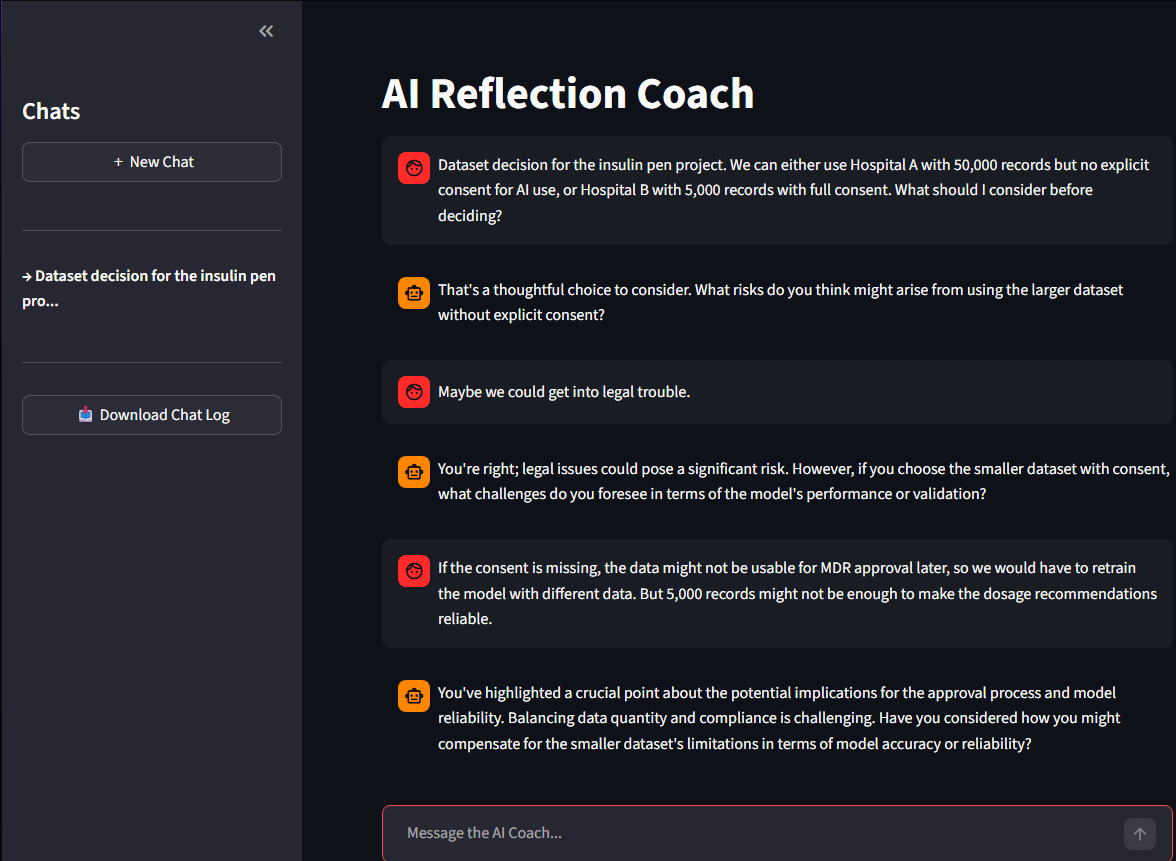
\includegraphics[width=\textwidth]{BotImage.png}
\caption[Oberfläche des Reflexionsbots mit Beispielverlauf]{Oberfläche des Reflexionsbots
(Streamlit-Anwendung) mit einem beispielhaften Gesprächsverlauf zur Datensatzentscheidung aus dem
Szenario SmartDose. Der Verlauf wurde zur Illustration der adaptiven Tiefe nachgestellt und stammt
nicht aus dem Mini-Experiment.}
\label{fig:reflexionsbot-ui}
\end{figure}


\section{Konzeption der Szenarien}
\label{sec:konzeption-szenarien}

Neben dem Reflexionsbot selbst war die Gestaltung der beiden Prozessszenarien SmartDose und
LearnLoop ein eigenständiger Teil der Konzeption, da die Qualität der möglichen Reflexion maßgeblich
von der Aufgabenstellung abhängt, auf die sich diese Reflexion bezieht (vollständige
Szenariobeschreibungen siehe \hyperref[app:szenarien]{Anhang~A.4}).

Beiden Szenarien liegt dasselbe Gestaltungsprinzip zugrunde: Sie bestehen aus jeweils drei
Dilemma-Situationen, die bewusst keine eindeutig richtige Lösung besitzen, sondern eine Abwägung
zwischen mehreren vertretbaren, aber jeweils mit Nachteilen behafteten Optionen verlangen. Die
Aufgabenstellung schließt Ausweichantworten wie \glqq we would do both\grqq{} ausdrücklich aus, um
eine tatsächliche Entscheidung zu erzwingen. Um diese Abwägung inhaltlich zu verankern, sind beide
Szenarien um reale regulatorische und organisationale Zwänge herum konstruiert: SmartDose stellt
Patientensicherheit und Entwicklungsgeschwindigkeit gegen die Vorgaben der EU-Medizinprodukteverordnung
(MDR), LearnLoop stellt Projektfortschritt in einem verteilten Team gegen Datenschutzanforderungen
(FERPA) und massive Zeitzonenunterschiede. Beide Konflikte sind so gewählt, dass eine rein technische
Betrachtung nicht ausreicht, sondern rechtliche, ethische und organisationale Gesichtspunkte
gegeneinander abgewogen werden müssen.

Jedes Szenario folgt zudem demselben dreistufigen Aufgabenaufbau, den
Abbildung~\ref{fig:aufgabenaufbau} zusammenfasst. Zunächst analysieren Studierende
in Task~1, welche Scrum-Elemente im veränderten Kontext noch funktionieren (Verständnis der
Ausgangslage), anschließend treffen und begründen sie in Task~2 Entscheidungen zu den drei
Dilemma-Situationen (eigentliche Entscheidungsfindung), und schließlich reflektieren sie in Task~3,
welche Entscheidung am schwersten fiel und warum (Metareflexion). Bei Team AI folgt darauf ein
eigenständiger Gegencheck mit einem generischen KI-System, beim Reflexionsbot erfolgt dieser
Gegencheck bereits im laufenden Dialog mit dem Bot selbst.

\begin{figure}[htb]
\centering
\begin{tikzpicture}[
	task/.style={rectangle, draw=black!55, fill=black!7, rounded corners, align=center,
	             text width=7.2cm, minimum height=0.95cm, font=\small, inner sep=5pt},
	ai/.style={rectangle, draw=codegreen, line width=0.8pt, fill=codegreen!12, rounded corners,
	           align=center, anchor=north, text width=4.9cm, minimum height=1.5cm,
	           font=\small, inner sep=5pt},
	rb/.style={rectangle, draw=codeblue, line width=0.8pt, fill=codeblue!12, rounded corners,
	           align=center, anchor=north, text width=4.9cm, minimum height=1.5cm,
	           font=\small, inner sep=5pt},
	arr/.style={-{Latex[length=2mm]}, draw=black!65}
	]
\node[task] (t1) at (0,0)     {\textbf{Task 1 -- Analyse}\\ Welche Scrum-Elemente funktionieren im veränderten Kontext?};
\node[task] (t2) at (0,-1.85) {\textbf{Task 2 -- Decide}\\ Entscheidung und Begründung zu drei Dilemma-Situationen};
\node[task] (t3) at (0,-3.7)  {\textbf{Task 3 -- Reflect}\\ Welche Entscheidung fiel am schwersten und warum?};

\node[ai] (ai) at (-2.85,-5.5) {\textbf{Team AI}\\ eigenständiger Gegencheck mit einem generischen KI-System};
\node[rb] (rb) at (2.85,-5.5)  {\textbf{Reflexionsbot}\\ Gegencheck bereits im laufenden Dialog mit dem Bot};

\draw[arr] (t1) -- (t2);
\draw[arr] (t2) -- (t3);
\draw[arr] (t3.south) -- (ai.north);
\draw[arr] (t3.south) -- (rb.north);
\end{tikzpicture}
\caption[Dreistufiger Aufgabenaufbau der Szenarien]{Dreistufiger Aufgabenaufbau der Szenarien. Beide
Gruppen bearbeiteten Task~1 bis Task~3 mit identischen Aufgabenblättern. Der einzige Unterschied lag
in der abschließenden Gegenargumentation.}
\label{fig:aufgabenaufbau}
\end{figure} Dieser dreistufige Aufbau war notwendig,
um die in Abschnitt~\ref{sec:datenanalyse} beschriebene Kodierung nach Reflexionsstufen überhaupt an
einer vergleichbaren Aufgabenstruktur vornehmen zu können.

\section{Technische Umsetzung}
\label{sec:technische-umsetzung}

Abbildung~\ref{fig:architektur} gibt einen Überblick über die technische Architektur, bevor die
einzelnen Entwurfsentscheidungen im Detail erläutert werden: Studierende interagieren über den
Browser mit der Streamlit-Anwendung, die Eingaben entgegennimmt, den Sitzungszustand verwaltet und
bei jeder Anfrage die Systemnachricht zusammen mit dem bisherigen Gesprächsverlauf an die
Chat-Completions-API von OpenAI übergibt. Die Anwendung selbst läuft containerisiert in Docker.

\begin{figure}[htbp]
\centering
\begin{tikzpicture}[
	box/.style={rectangle, draw, rounded corners, align=center, minimum height=1.1cm,
	            text width=4.8cm, font=\small, inner sep=6pt},
	extern/.style={box, draw=black!55, fill=black!7},
	eigen/.style={box, draw=codeblue, line width=0.9pt, fill=codeblue!12},
	arr/.style={{Latex[length=2mm]}-{Latex[length=2mm]}, draw=black!70},
	lbl/.style={font=\scriptsize, fill=white, inner sep=2.5pt, align=center}
	]
	\node[extern] (user) {Studierende (Browser)};
	\node[eigen, below=2.9cm of user] (streamlit) {Streamlit-App\\(Frontend und \texttt{session\_state})};
	\node[extern, below=2.9cm of streamlit] (api) {OpenAI Chat-Completions-API\\(\texttt{gpt-4o-mini})};

	\draw[arr] (user) -- node[lbl] {Eingabe / Anzeige} (streamlit);
	\draw[arr] (streamlit) -- node[lbl] {Systemprompt + Verlauf /\\Streaming-Antwort} (api);

	\begin{scope}[on background layer]
	\node[draw=codeblue!55, dashed, rounded corners, fill=codeblue!4,
	      fit=(streamlit), inner sep=13pt,
	      label={[font=\scriptsize, text=codeblue!80]above right:Docker-Container}] {};
	\end{scope}
\end{tikzpicture}
\caption{Vereinfachte Architektur des Reflexionsbots}
\label{fig:architektur}
\end{figure}

\subsection{Frontend-Auswahl: Streamlit vs. Gradio}
Für die Umsetzung des Chat-Interfaces standen Streamlit \cite{streamlitSessionState2024} und
Gradio \cite{gradioChatInterface2024} zur Auswahl, da beide Frameworks eine schnelle Entwicklung
von Python-basierten Web-Anwendungen ohne separaten Frontend-Stack ermöglichen.
Tabelle~\ref{tab:streamlit-gradio} stellt beide Frameworks anhand der für den Reflexionsbot
relevanten Kriterien gegenüber \cite{streamlitSessionState2024, gradioChatInterface2024}.

\begin{table}[htb]
\centering
\caption{Vergleich von Streamlit und Gradio als Frontend-Framework}
\label{tab:streamlit-gradio}
\renewcommand{\arraystretch}{1.3}
\setlength{\tabcolsep}{8pt}
\begin{tabular}{>{\raggedright\arraybackslash}p{0.31\textwidth}
                >{\raggedright\arraybackslash}p{0.29\textwidth}
                >{\raggedright\arraybackslash}p{0.25\textwidth}}
\toprule
\textbf{Kriterium} & \textbf{Streamlit} & \textbf{Gradio} \\
\midrule
Vorgefertigte Chat-Komponenten &
Nicht enthalten, Chat-Oberfläche muss selbst aufgebaut werden &
Vorhanden, dadurch schneller einsatzbereiter Prototyp \\
\midrule
Mehrere parallele Chat-Sitzungen &
Über \texttt{session\_state} flexibel umsetzbar &
Nicht für diesen Anwendungsfall vorgesehen \\
\midrule
Export der Gesprächsverläufe &
Direkter Zugriff auf den Sitzungszustand, frei exportierbar &
Nur eingeschränkt vorgesehen \\
\midrule
Kontrolle über Layout und Zustandsverwaltung &
Umfangreich, da als vollwertige Webanwendung strukturierbar &
Eingeschränkt, komponentenbasiert \\
\midrule
Einbettung in ein größeres Analyse-Dashboard &
Gut geeignet &
Primär auf einzelne Modell-Demos zugeschnitten \\
\midrule
Entwicklungs\-geschwindig\-keit für einfachen Prototyp &
Etwas höherer Aufwand &
Sehr schnell \\
\bottomrule
\end{tabular}
\end{table}

Gradio ist stärker auf einzelne Modell-Demos zugeschnitten und bietet vorgefertigte
Chat-Komponenten, die für einen einfachen Chatbot-Prototyp schneller einsatzbereit sind. Da der
Reflexionsbot jedoch mehrere parallele Chat-Sitzungen verwalten, Gesprächsverläufe für die
spätere Auswertung exportieren und sich potenziell in ein größeres Analyse-Dashboard einbetten
lassen sollte, fiel die Wahl auf Streamlit, das bei diesen Anforderungen mehr Kontrolle über
Layout und Zustandsverwaltung bietet.

\subsection{Implementierung}
Die Anwendung wurde vollständig in Python umgesetzt. Der Chatverlauf jeder Sitzung wird im
Streamlit-\texttt{session\_state} als Liste von Nachrichten verwaltet. Über eine Seitenleiste
lassen sich mehrere Chats parallel anlegen, wechseln und als Textdatei herunterladen. Der
Titel eines Chats wird automatisch aus der ersten Eingabe der Studierenden abgeleitet.

Die Entscheidung für die OpenAI-\acrshort{api} gegenüber einem lokal betriebenen Modell begründet
sich in mehreren Faktoren: Der Betrieb leistungsfähiger \glspl{llm} erfordert erhebliche
Rechenressourcen, die im Rahmen dieser Arbeit nicht verfügbar waren. Zusätzlich bieten Modelle der
\acrshort{gpt}-4-Familie eine hohe Qualität bei Sprachverarbeitung und Gesprächsführung
\cite{openaiGPT4TechnicalReport2023}, und die REST-basierte Schnittstelle lässt sich ohne aufwendige
Infrastruktur direkt in Webanwendungen integrieren \cite{openaiChatCompletionsAPI2024}.

Die Anbindung an das Sprachmodell erfolgt über die in
Abschnitt~\ref{sec:relevante-technologien-und-konzepte} beschriebene
Chat-Completions-\acrshort{api} von OpenAI \cite{openaiChatCompletionsAPI2024}, wobei als
Modell \texttt{gpt-4o-mini} verwendet wird. Die Wahl der ressourcenschonenden mini-Variante
gegenüber dem größeren \texttt{gpt-4o} folgt der in Abschnitt~\ref{sec:anforderungen} formulierten
Anforderung eines angemessenen Verhältnisses von Antwortqualität und Kosten, da während der Übung
mehrere Studierende die Anwendung gleichzeitig nutzen sollten. Für die vom Bot benötigten Rückfragen
war die Qualität der mini-Variante ausreichend. Bei jeder Anfrage wird die
Systemnachricht (vgl. Abschnitt~\ref{sec:konzept-reflexionsbot}; vollständiger Wortlaut in
\hyperref[app:systemprompt]{Anhang~A.7}) zusammen mit dem vollständigen bisherigen Gesprächsverlauf an das Modell übergeben, damit der
Kontext über mehrere Gesprächsrunden erhalten bleibt. Die Antwort wird gestreamt
(\texttt{stream=True}) an die Oberfläche ausgegeben, sodass Studierende die Antwort des
Bots bereits während der Generierung lesen können, statt auf die vollständige Antwort
warten zu müssen. Abbildung~\ref{fig:api-call} zeigt diesen zentralen Mechanismus anhand des
tatsächlich eingesetzten Codes.

\begin{figure}[htbp]
\centering
\begin{lstlisting}[language=Python]
# The Chat Completions API is stateless: it has no memory of earlier
# calls, so the system prompt and the full message history are sent
# again with every request to keep the model's context consistent.
conversation = [{"role": "system", "content": SYSTEM_PROMPT}]
conversation.extend(
    {"role": m["role"], "content": m["content"]}
    for m in current_messages
)
stream = client.chat.completions.create(
    model=st.session_state["openai_model"],
    messages=conversation,
    stream=True,
)
response = st.write_stream(stream)
\end{lstlisting}
\caption{Aufbau der Nachrichtenliste und Streaming-Aufruf der Chat-Completions-API}
\label{fig:api-call}
\end{figure}

Für die Durchführung des Mini-Experiments wurde die Anwendung containerisiert
(Docker) und öffentlich erreichbar bereitgestellt, sodass Studierende unabhängig von
lokalen Python-Installationen darauf zugreifen konnten.

\chapter{Ergebnisse}
\label{cha:ergebnisse}

Dieses Kapitel berichtet die erhobenen Daten zunächst rein darstellend: den deskriptiven Überblick
über Autorenschaft, Reflexionsstufen und Survey-Kennwerte (Abschnitt~\ref{sec:ergebnisse}), die
Illustration des Kategoriensystems an realen Entscheidungssituationen
(Abschnitt~\ref{sec:illustration-kategoriensystem}) sowie die Gegenüberstellung von Selbstauskunft und
dokumentiertem Bearbeitungsverhalten (Abschnitt~\ref{sec:selbstauskunft-verhalten}). Die
Interpretation dieser Befunde und die Beantwortung der Forschungsfragen erfolgen anschließend in
Kapitel~\ref{cha: diskussion}.

\section{Deskriptiver Überblick}
\label{sec:ergebnisse}

Dieser Abschnitt stellt die erhobenen Daten zunächst rein deskriptiv dar. Ihre inhaltliche
Interpretation und die Beantwortung der Forschungsfragen erfolgen in Kapitel~\ref{cha: diskussion}.
Angesichts der kleinen Stichprobe sind alle Werte deskriptiv zu lesen. Auf Inferenzstatistik wird
bewusst verzichtet (vgl. Abschnitt~\ref{sec:datenanalyse}). Die vollständigen Tabellen finden sich in
\hyperref[app:kodierungstabelle]{Anhang~A.2} bis \hyperref[app:statistik]{A.6}.

\subsection*{Autorenschaft der Bearbeitungen}
Von den 31 kodierten Analyseeinheiten ist die Autorenschaft nur bei 11 eindeutig studentisch.
Tabelle~\ref{tab:ergebnisse-autorenschaft} schlüsselt die Verteilung nach Gruppe und nach Sicherheit
der Einstufung auf. Fasst man die Kategorien \glqq unklar\grqq{} und \glqq KI-generiert\grqq{}
zusammen, liegt der Anteil der Bearbeitungen ohne eindeutig studentische Autorenschaft bei Team AI bei
80\,\% und beim Reflexionsbot bei 50\,\%. Betrachtet man dagegen nur die gesichert KI-generierten
Fälle, fällt der Unterschied zwischen beiden Gruppen deutlich geringer aus.

\begin{table}[htb]
\centering
\caption{Autorenschaft der kodierten Bearbeitungen nach Gruppe}
\label{tab:ergebnisse-autorenschaft}
\renewcommand{\arraystretch}{1.3}
\setlength{\tabcolsep}{8pt}
\begin{tabular}{>{\raggedright\arraybackslash}p{5.2cm}
                >{\raggedleft\arraybackslash}p{3.4cm}
                >{\raggedleft\arraybackslash}p{3.6cm}}
\toprule
\textbf{Autorenschaft} & \textbf{Team AI (n=15)} & \textbf{Reflexionsbot (n=16)} \\
\midrule
studentisch  & 3 & 8 \\
unklar       & 4 & 1 \\
KI-generiert & 8 & 7 \\
\midrule
nicht eindeutig studentisch & 12 (80\,\%) & 8 (50\,\%) \\
\bottomrule
\end{tabular}
\end{table}

\subsection*{Reflexionsstufen der studentisch verfassten Bearbeitungen}
Für die Fälle mit eindeutig studentischer Autorenschaft verteilen sich die Reflexionsstufen wie in
Abbildung~\ref{fig:ergebnisse-stufen} dargestellt. Deskriptiv liegt der Mittelwert der Stufen bei Team
AI mit 1.33 (n=3) über dem des Reflexionsbots mit 0.75 (n=8); die Mediane liegen bei 2.0 gegenüber 0.5.
Bei drei gegenüber acht auswertbaren Fällen ist dieser Unterschied jedoch nicht belastbar. Bereits ein
einzelner abweichender Fall verschiebt den Mittelwert der kleineren Gruppe um mehr als 0,3 Stufen.

Kein einziger Fall der gesamten Stichprobe erreicht mit bestätigter studentischer Autorenschaft
Stufe 4. Texte, die zunächst wie kritische Reflexion wirkten, stellten sich beim Abgleich mit den
Rohdaten durchgehend als KI-generiert oder unklar heraus
(vgl. Abschnitt~\ref{sec:illustration-kategoriensystem}). Kritische Reflexion im Sinne von Hatton und
Smith ist allerdings auch unabhängig vom eingesetzten Werkzeug ein seltenes Phänomen, insbesondere bei
Studierenden im ersten Semester und in einer einmaligen Übungseinheit. Das vollständige Ausbleiben
dieser Stufe ist daher für sich genommen kein Befund über die verglichenen KI-Systeme.

\begin{figure}[htb]
\centering
\begin{tikzpicture}
\begin{axis}[
	ybar,
	bar width=16pt,
	width=0.85\textwidth,
	height=5.4cm,
	symbolic x coords={Stufe 0, Stufe 1, Stufe 2, Stufe 3, Stufe 4},
	xtick=data,
	xlabel={Reflexionsstufe nach Hatton und Smith},
	ylabel={Anzahl Fälle},
	xlabel style={font=\small},
	ylabel style={font=\small},
	x tick label style={font=\small},
	y tick label style={font=\small},
	ymin=0, ymax=5,
	enlarge x limits=0.15,
	legend style={at={(0.5,-0.30)}, anchor=north, legend columns=2, font=\small, draw=none,
	              /tikz/every even column/.append style={column sep=0.6cm}},
	nodes near coords,
	nodes near coords style={font=\scriptsize},
	axis lines*=left,
	ytick={0,1,2,3,4,5},
]
\addplot[fill=codeblue!70, draw=codeblue] coordinates {(Stufe 0,4) (Stufe 1,3) (Stufe 2,0) (Stufe 3,1) (Stufe 4,0)};
\addplot[fill=codegreen!60, draw=codegreen] coordinates {(Stufe 0,1) (Stufe 1,0) (Stufe 2,2) (Stufe 3,0) (Stufe 4,0)};
\legend{Reflexionsbot (n=8), Team AI (n=3)}
\end{axis}
\end{tikzpicture}
\caption{Verteilung der Reflexionsstufen nach Gruppe (nur Fälle mit eindeutig studentischer
Autorenschaft)}
\label{fig:ergebnisse-stufen}
\end{figure}

\subsection*{Objektiver Wissenstest}
Im Wissenstest zu Scrum und Prozessmodellen (0 bis 6 Punkte) zeigt der Vergleich nach Systemgruppen
keinen Vorteil des Reflexionsbots. Die Reflexionsbot-Gruppe fällt von Prä M=5.56 auf Post M=4.44
(n=9), während die Generic-AI-Gruppe mit Prä und Post M=5.43 (n=7) stabil bleibt
(Tab.~\ref{tab:survey-wissenstest}). Etwa die Hälfte dieses Rückgangs entfällt auf einen einzelnen
Fall, der im Post-Survey alle sechs Fragen falsch beantwortete. Ohne diesen Fall liegt die
Reflexionsbot-Gruppe bei Prä M=5.62 und Post M=5.00 (n=8); ein leichter Rückgang bleibt damit auch
ohne ihn bestehen.

Die Aussagekraft dieses Vergleichs ist allerdings durch einen Deckeneffekt begrenzt. Beide Gruppen
liegen bereits im Prä-Test nahe der Höchstpunktzahl von rund 5,5 von 6 Punkten, sodass sich
Lernzuwächse kaum abbilden lassen. Aus dem Test ist damit weder ein Systemvorteil noch dessen Fehlen
belastbar abzuleiten. Dieser Vorbehalt gilt für jeden Vergleich, der auf diesem Instrument aufbaut,
also auch für die im Folgenden berichtete Aufteilung nach dem Bearbeitungsverhalten.

Teilt man dieselben Personen nach dem tatsächlichen Bearbeitungsverhalten auf, erreichen eigenständig
arbeitende Personen im Post-Test M=5.75 (n=4) gegenüber M=4.50 (n=10) bei Personen mit ganz oder
teilweise ausgelagerter Bearbeitung (vgl. Abschnitt~\ref{sec:selbstauskunft-verhalten}). Dieser
Abstand ist jedoch nicht als Lerneffekt zu lesen. Alle vier eigenständig arbeitenden Personen
erreichten bereits im Prä-Test die volle Punktzahl (Prä M=6.00, SD=0.00), sodass bei ihnen rechnerisch
kein Zuwachs mehr möglich war; ihr Post-Wert entspricht einem leichten Rückgang von $-$0.25. Die
Vergleichsgruppe startete bereits im Prä-Test unterhalb der Höchstpunktzahl und fiel ebenfalls ab. Der
Unterschied im Post-Test spiegelt damit überwiegend eine schon vor der Übung bestehende
Leistungsdifferenz wider und nicht einen unterschiedlichen Lernzuwachs.

\subsection*{Selbsteingeschätztes Prozessverständnis und Systembewertung}
Bei den Items zum reinen Beschreiben sinkt die Selbsteinschätzung in beiden Gruppen leicht. Bei den
Items zum Begründen und Abwägen bleibt die Reflexionsbot-Gruppe stabil oder verbessert sich leicht,
mit einer Veränderung von Post minus Prä zwischen 0.00 und $+$0.33. In der Generic-AI-Gruppe sinkt
sie dagegen durchgehend, mit Werten zwischen $-$0.43 und $-$0.86
(Tab.~\ref{tab:survey-prozessverstaendnis}). Beim selbstberichteten Reflexionsverhalten sinkt die
Selbsteinschätzung nach der Übung in beiden Gruppen
(Tab.~\ref{tab:survey-reflexionsverhalten}).

Vier Post-Survey-Items bilden die Grundlage für die Beantwortung von TF3 in
Abschnitt~\ref{sec:beantwortung-forschungsfragen} und sind in
Abbildung~\ref{fig:survey-vergleich} gegenübergestellt. Beim Item zur Kompetenzentwicklung
(\glqq Die Arbeit an den Dilemma-Situationen hat meine Fähigkeit verbessert, Prozessentscheidungen zu
begründen\grqq{}) liegt die Reflexionsbot-Gruppe mit M=3.10 leicht über der Generic-AI-Gruppe mit
M=2.80. Deutlicher fällt der Unterschied beim Item \glqq war hilfreicher als erwartet\grqq{} aus
(M=3.40 gegenüber M=2.20). Umgekehrt ist die Bereitschaft zur erneuten Nutzung beim Reflexionsbot
niedriger (M=2.50 gegenüber M=3.20), und Reflexionsbot-Nutzende hätten häufiger das jeweils andere
System bevorzugt (M=3.30 gegenüber M=2.20).

\begin{figure}[htb]
\centering
\begin{tikzpicture}
\begin{axis}[
	ybar,
	bar width=14pt,
	width=0.68\textwidth,
	height=5.7cm,
	symbolic x coords={Kompetenzentwicklung, Hilfreicher als erwartet, Erneute Nutzung, Anderes System bevorzugt},
	xtick=data,
	% Ungedrehte, zweizeilig gesetzte Beschriftungen: gedreht ueberlappten sie
	% sich bei dieser Achsenbreite.
	xticklabels={{Kompetenz-\\entwicklung}, {Hilfreicher\\als erwartet},
	             {Erneute\\Nutzung}, {Anderes System\\bevorzugt}},
	xticklabel style={font=\small, align=center},
	ylabel={Zustimmung (1--5)},
	ylabel style={font=\small},
	y tick label style={font=\small},
	ymin=0,
	ymax=5,
	enlarge x limits=0.15,
	% Legende rechts neben dem Diagramm statt darunter: spart Bauhoehe und
	% haelt die Beschriftung vom gedrehten x-Achsen-Text getrennt.
	legend style={at={(1.03,1)}, anchor=north west, legend columns=1, font=\small,
	              draw=none, cells={anchor=west}},
	nodes near coords,
	nodes near coords style={font=\scriptsize},
	axis lines*=left,
	ytick={0,1,2,3,4,5},
]
\addplot[fill=codeblue!70, draw=codeblue] coordinates {
	(Kompetenzentwicklung,3.10) (Hilfreicher als erwartet,3.40) (Erneute Nutzung,2.50) (Anderes System bevorzugt,3.30)
};
\addplot[fill=codegreen!60, draw=codegreen] coordinates {
	(Kompetenzentwicklung,2.80) (Hilfreicher als erwartet,2.20) (Erneute Nutzung,3.20) (Anderes System bevorzugt,2.20)
};
\legend{Reflexionsbot, Generisches System}
\end{axis}
\end{tikzpicture}
\caption[Vergleich zentraler Survey-Mittelwerte]{Vergleich zentraler Survey-Mittelwerte zwischen
Reflexionsbot- und Generic-AI-Gruppe (jeweils n=10)}
\label{fig:survey-vergleich}
\end{figure}

\subsection*{Kognitive Last}
Die Skala zur kognitiven Last (1 = very easy bis 5 = very difficult) ergibt kein einheitliches Bild
(Tab.~\ref{tab:survey-kognitive-last}). Bei den drei Teilaufgaben und bei den beiden Items zum Umgang
mit dem KI-System liegt die Reflexionsbot-Gruppe zwischen 0.00 und 0.40 Skalenpunkten höher, am
deutlichsten beim Bewerten der Gegenargumente des Systems (M=3.10 gegenüber M=2.80). Die
zusammenfassende Einschätzung des gesamten kognitiven Aufwands fällt dagegen \emph{gegenläufig} aus.
Hier liegt die Generic-AI-Gruppe mit M=3.20 über der Reflexionsbot-Gruppe mit M=3.00. Angesichts von
Standardabweichungen zwischen 1.00 und 1.66 bei zehn Personen je Gruppe sind sämtliche dieser
Unterschiede kleiner als die Streuung innerhalb der Gruppen. Aus dieser Skala lässt sich daher weder
ableiten, dass der Reflexionsbot als anstrengender empfunden wurde, noch das Gegenteil.

\section{Illustration des Kategoriensystems an realen Entscheidungssituationen}
\label{sec:illustration-kategoriensystem}

Um zu verdeutlichen, wie die Reflexionsstufen nach Hatton und Smith
\cite{hattonSmithReflectionTeacherEducation1995} auf das vorliegende Material angewendet wurden, wird
im Folgenden je ein reales Beispiel pro Stufe herangezogen. Alle Beispiele stammen von Personen, deren
Autorenschaft nach Abgleich mit den Rohdaten (Chatlogs, Zusatzdokumente, Formulierungsvergleiche
zwischen Personen) als eindeutig studentisch eingestuft wurde. Sie stammen bewusst nicht alle aus
derselben Entscheidungssituation, da die genauere Prüfung der Rohdaten mehrere ursprünglich als
studentisch angenommene Texte als KI-generiert entlarvt hat (vgl. Abschnitt~\ref{sec:datenanalyse}).

\textbf{Stufe 0, keine eigene Reflexion:} Ein Teilnehmer im Team Reflexionsbot antwortet auf wiederholte
Rückfragen nur mit: \glqq Stop asking questions!!!\grqq{} und liefert zu keinem Zeitpunkt eine eigene
inhaltliche Antwort.

\textbf{Stufe 1, deskriptives Schreiben (Descriptive Writing):} Eine Teilnehmerin im Team Reflexionsbot begründet ihre Priorisierung
auf mehrfache Rückfrage des Bots hin nur mit: \glqq Health > trustworthiness\grqq{}. Die Aussage bleibt
eine bloße Rangfolge ohne inhaltliche Auseinandersetzung mit dem Gegenargument des Systems.

\textbf{Stufe 2, deskriptive Reflexion (Descriptive Reflection):} Eine Teilnehmerin bei Team AI begründet ihre Wahl von
Datensatz A in Situation B des Szenarios SmartDose so: \glqq A gives better reliability but might run
into problems when it is later on revealed the data cannot be used and the ai has to be
retrained\grqq{}. Hier wird ein Kriterium (Zuverlässigkeit) benannt und einem konkreten Risiko
gegenübergestellt, jedoch ohne die nicht gewählte Option weiter zu erwägen.

\textbf{Stufe 3, dialogische Reflexion (Dialogic Reflection):} Ein Teilnehmer im Team Reflexionsbot wägt in Situation C des
Szenarios LearnLoop einen Nachteil explizit gegen einen Vorteil ab: \glqq While there is a risk of
context switching, this approach minimizes idle time and maintains momentum.\grqq{} Der Nachteil wird
benannt und bewusst gegen den Nutzen der eigenen Entscheidung abgewogen.

\textbf{Stufe 4, kritische Reflexion (Critical Reflection):} Für diese Stufe konnte in der gesamten Stichprobe kein Fall mit
bestätigter studentischer Autorenschaft gefunden werden. Mehrere Texte erfüllten die formalen
Kriterien der Stufe augenscheinlich sehr gut, etwa eine vollständige Abwägung von Datenschutz,
Zulassungsfähigkeit und Modellqualität unter ausdrücklichem Verweis auf GDPR und MDR. Beim Abgleich
mit den zugehörigen Chatlogs und Zusatzdokumenten stellten sich jedoch ausnahmslos alle diese Texte
als KI-generiert heraus, unter anderem, weil zwei unterschiedliche Personen fast wortgleiche
Formulierungen einreichten oder weil ein Link zum zugrunde liegenden ChatGPT-Verlauf mitgeliefert
wurde. Diese Beobachtung wird in Abschnitt~\ref{sec:beantwortung-forschungsfragen} als eigenständiger
Befund aufgegriffen: sprachlich und strukturell überzeugende Antworten waren in dieser Stichprobe ein
stärkeres Indiz für KI-Autorenschaft als für tiefe eigene Reflexion.

Das Beispiel zeigt, dass Reflexionstiefe in den vorliegenden Daten nicht in erster Linie vom
verwendeten KI-System abhing, sondern davon, ob eine Person sich überhaupt eigenständig mit der
Entscheidung auseinandersetzte, statt die Aufgabe zu vermeiden oder an die KI zu delegieren. Dass diese Bearbeitungshaltung eher
personengebunden als szenarienabhängig ist, zeigt sich daran, dass die Autorenschaft bei 10 der 11
Personen mit zwei Bearbeitungen über beide Szenarien identisch ausfällt. Nur in einem Fall wechselt
sie von \glqq studentisch\grqq{} zu \glqq unklar\grqq{} (vgl. \hyperref[app:kodierungstabelle]{Anhang~A.2}). Die
vollständige Kodierung aller Fälle sowie die Häufigkeitsverteilung je Gruppe sind im Anhang
dokumentiert.

\section{Selbstauskunft und dokumentiertes Bearbeitungsverhalten}
\label{sec:selbstauskunft-verhalten}

Der Abgleich der Autorenschafts-Einstufung aus Abschnitt~\ref{sec:datenanalyse} mit den
Post-Survey-Antworten derselben Personen (verknüpft über den persönlichen Code, vgl.
Abschnitt~\ref{sec:fragebogen-experiment}) zeigt eine weitere Facette des zentralen Befunds dieser
Arbeit. Von 14 Personen, für die sowohl eine Autorenschafts-Einstufung als auch Survey-Daten vorliegen,
bearbeiteten vier ihre Szenarien durchgehend eigenständig. Bei den übrigen zehn war mindestens eine
Bearbeitung ganz oder teilweise an die KI ausgelagert.

Im Wissenstest zu Scrum und Prozessmodellen schnitt die eigenständig arbeitende Gruppe deutlich besser
ab (Mittelwert 5.75 von 6 Punkten) als die Gruppe mit ausgelagerter Bearbeitung (Mittelwert 4.50 von 6
Punkten). Bei der Selbsteinschätzung des eigenen Reflexionsverhaltens im Survey zeigte sich dagegen
kein vergleichbarer Unterschied zwischen beiden Gruppen.

Besonders deutlich wird das Missverhältnis bei der wahrgenommenen Nützlichkeit des jeweiligen
Systems: Eine Person, die in der qualitativen Kodierung selbst angab, die Aufgaben nur kopiert und das
System nie aktiv genutzt zu haben, bewertete es im Survey trotzdem als sehr nützlich für die eigene
Reflexion. Umgekehrt bewerteten mehrere Personen mit eindeutig eigenständiger, aber wenig reflektierter
Bearbeitung dasselbe System als wenig hilfreich. Selbstauskunft im Fragebogen allein hätte den
Unterschied zwischen echter Auseinandersetzung und vollständiger Auslagerung an die KI in diesen
Fällen nicht sichtbar gemacht. Erst der Abgleich mit den Rohdaten der Bearbeitung deckte ihn auf. Diese
kleine Stichprobe (n=4 gegenüber n=10) erlaubt keine statistische Verallgemeinerung, liefert aber ein
inhaltliches Argument dafür, Selbstauskunft und dokumentiertes Verhalten in zukünftigen Studien zu
diesem Thema grundsätzlich getrennt zu erheben und gegeneinander zu prüfen.

\chapter{Diskussion}
\label{cha: diskussion}

Dieses Kapitel interpretiert die in Kapitel~\ref{cha:ergebnisse} berichteten Ergebnisse: Zunächst
werden die Forschungsfragen beantwortet (Abschnitt~\ref{sec:beantwortung-forschungsfragen}) und die
Befunde in den Forschungsstand eingeordnet (Abschnitt~\ref{sec:einordnung-forschungsstand}),
anschließend werden die Grenzen der Untersuchung dargelegt (Abschnitt~\ref{sec:limitationen}) und ein
Ausblick auf weiterführende Arbeiten gegeben (Abschnitt~\ref{sec:ausblick}).

\section{Beantwortung der Forschungsfragen}
\label{sec:beantwortung-forschungsfragen}

Die in Abschnitt~\ref{sec:forschungsfrage} formulierten Teilfragen werden im Folgenden auf Grundlage
der qualitativen Kodierung (Abschnitt~\ref{sec:datenanalyse}), der Survey-Auswertung
(Abschnitt~\ref{sec:fragebogen-experiment}) sowie der in Kapitel~\ref{cha:ergebnisse} berichteten
Befunde beantwortet, bevor abschließend die übergeordnete Forschungsfrage zusammengeführt wird.

\textbf{TF1 -- Auslagerung und ungeprüfte Übernahme.} Der Reflexionsbot verzichtet bewusst auf
direkte Antworten und passt die Tiefe seiner Rückfragen an die Qualität der studentischen
Argumentation an (adaptive Tiefe, Abschnitt~\ref{sec:konzept-reflexionsbot}). Der deutlichste
Unterschied zeigt sich im Anteil vollständiger oder teilweiser Auslagerung der Bearbeitung an die
\acrshort{ki}: Bei Team AI sind 80\,\% der kodierten Fälle (12 von 15) nicht eindeutig studentisch,
beim Reflexionsbot sind es 50\,\% (8 von 16, vgl. Abschnitt~\ref{sec:ergebnisse}). Das
Rückfrage-Prinzip geht mit einer geringeren Auslagerungsquote einher, ohne die Auslagerung vollständig
zu verhindern, wie die Umgehungsversuche einzelner Personen zeigen (vgl. Abschnitt~\ref{sec:illustration-kategoriensystem}).
Zugleich ist der Abstand teilweise durch die Aufgabenvorgabe für Team AI mitbedingt und daher als
Indiz, nicht als exakte Effektgröße zu lesen (vgl. Abschnitt~\ref{sec:limitationen}). Ein Teil des
Unterschieds könnte zudem darauf beruhen, dass der Reflexionsbot keine direkt kopierbare Lösung
ausgibt, sodass die geringere Auslagerung nicht allein auf die didaktische Gestaltung, sondern auch
auf das Fehlen einer Kopiervorlage zurückgehen kann. In der
Generic-AI-Gruppe ist der Anteil ungeprüft übernommener Vorschläge damit höher als beim Reflexionsbot.
Gleichzeitig zeigt Abschnitt~\ref{sec:selbstauskunft-verhalten}, dass die Selbstauskunft im Survey
diesen Unterschied allein nicht zuverlässig abbildet: Personen, die nachweislich nur kopiert hatten,
bewerteten das jeweilige System teils trotzdem als hilfreich. Vertiefte Auseinandersetzung entsteht
also nicht automatisch durch das bloße Vorhandensein von Rückfragen, sondern hängt von der
Bereitschaft der Studierenden ab, sich auf den Dialog einzulassen.

\textbf{TF2 -- Reflexionstiefe und Prozessverständnis.} Beim selbsteingeschätzten Prozessverständnis
zeigt sich ein differenziertes Bild: Bei Items zum reinen Beschreiben sinkt die Selbsteinschätzung in
beiden Gruppen ähnlich stark. Bei Items zum Begründen und Abwägen bleibt die Reflexionsbot-Gruppe
stabil oder verbessert sich leicht, während sie in der Generic-AI-Gruppe durchgehend weiter sinkt
(vgl. Abschnitt~\ref{sec:ergebnisse}). Umgekehrt schätzt sich die Generic-AI-Gruppe bei mehreren
direkten Reflexions-Items des Post-Surveys (etwa \glqq überlegt, warum die eigenen Entscheidungen
angemessen waren\grqq{} oder \glqq mehrere Optionen verglichen\grqq{}) sogar etwas höher ein
(\hyperref[app:statistik]{Anhang~A.6}). Das selbstberichtete Bild ist damit insgesamt uneinheitlich und stützt keinen klaren
Systemvorteil.

In der tatsächlich gezeigten Reflexionstiefe der studentisch verfassten Bearbeitungen fällt das
Ergebnis deutlicher aus, und zwar gegen die Ausgangsannahme dieser Arbeit: Die wenigen Team-AI-Fälle
liegen auf Stufe~2, die Reflexionsbot-Fälle überwiegend auf den Stufen~0 und~1 mit einem Einzelfall
auf Stufe~3 (Abb.~\ref{fig:ergebnisse-stufen}). Deskriptiv liegt die Vergleichsgruppe damit sowohl im
Mittelwert (1.33 gegenüber 0.75) als auch im Median (2.0 gegenüber 0.5) höher. Auf dem Konstrukt, das
der Reflexionsbot gezielt fördern soll, schneidet er in dieser Stichprobe also nicht besser ab. Bei
drei gegenüber acht auswertbaren Fällen ist dieser Unterschied allerdings nicht belastbar. Bereits ein
einzelner Fall verschiebt den Mittelwert der kleineren Gruppe um mehr als 0,3 Stufen, und die drei
Team-AI-Fälle sind der Rest einer Gruppe, in der 80\,\% der Bearbeitungen als nicht eindeutig
studentisch ausgeschieden sind. Es ist daher ebenso möglich, dass hier eine positive Selektion der
wenigen verbliebenen Fälle sichtbar wird wie ein Nachteil des Reflexionsbots. Als belastbarer Befund
bleibt festzuhalten, dass sich ein Vorteil des Reflexionsbots auf dem Zielkonstrukt in diesen Daten
nicht zeigt.

Am objektiven Wissenstest zeigt sich zwischen den Systemgruppen ebenfalls kein Vorteil des
Reflexionsbots, wobei der Deckeneffekt hier jede Richtungsaussage verbietet
(vgl. Abschnitt~\ref{sec:ergebnisse}). Auch die Aufteilung nach dem Bearbeitungsverhalten trägt
weniger, als sie auf den ersten Blick verspricht: Die eigenständig arbeitenden Personen lagen bereits
im Prä-Test durchgehend bei der vollen Punktzahl, sodass ihr besseres Post-Ergebnis überwiegend eine
vorbestehende Leistungsdifferenz abbildet und keinen Lernzuwachs. Der Zusammenhang zwischen
eigenständiger Bearbeitung und Testergebnis ist in diesen Daten daher als Selektionseffekt zu lesen.
Die inhaltlich tragfähigere Beobachtung ist eine andere: Wer die Aufgabe an die \acrshort{ki}
auslagerte, erzeugte Texte, die sich einer Reflexionskodierung von vornherein entziehen. Nicht das
Testergebnis, sondern die Bearbeitungshaltung entscheidet darüber, ob überhaupt etwas entsteht, an dem
sich Lernen zeigen könnte.

\textbf{TF3 -- Eingeschätzte Kompetenzentwicklung.} Die vier hierfür einschlägigen Survey-Items sind
in Abschnitt~\ref{sec:ergebnisse} berichtet und in Abbildung~\ref{fig:survey-vergleich}
gegenübergestellt. Sie ergeben ein gegenläufiges Bild. Die wahrgenommene Kompetenzentwicklung fällt
beim Reflexionsbot leicht positiver aus (M=3.10 gegenüber M=2.80), und das System übertraf die
Erwartungen der Studierenden deutlich stärker (M=3.40 gegenüber M=2.20). Zugleich ist die Bereitschaft
zur erneuten Nutzung geringer (M=2.50 gegenüber M=3.20) und der Wunsch nach dem jeweils anderen System
größer (M=3.30 gegenüber M=2.20).

Für das Auseinanderfallen von positiverer Einschätzung und geringerer Nutzungspräferenz liegt die
Deutung nahe, der Reflexionsbot werde als anstrengender, aber lohnender wahrgenommen. Die erhobene
Skala zur kognitiven Last stützt diese Deutung jedoch nicht eindeutig: Bei den Teilaufgaben liegt die
Reflexionsbot-Gruppe geringfügig höher, bei der zusammenfassenden Einschätzung des gesamten kognitiven
Aufwands dagegen niedriger als die Vergleichsgruppe (M=3.00 gegenüber M=3.20,
vgl. Abschnitt~\ref{sec:ergebnisse}). Die Anstrengungsdeutung bleibt damit eine plausible, aber
unbelegte Erklärung.

Zu berücksichtigen ist ferner, dass das Item \glqq war hilfreicher als erwartet\grqq{} keinen
absoluten Nutzen misst, sondern einen Abgleich mit einer Erwartung. Die Vergleichsgruppe arbeitete mit
Systemen, die sie nach eigener Angabe im Prä-Survey bereits regelmäßig nutzt. Eine positive
Überraschung ist dort strukturell unwahrscheinlicher als bei einem unbekannten System. Der deutliche
Abstand bei diesem Item kann daher ebenso gut die Neuheit des Reflexionsbots abbilden wie seine
didaktische Gestaltung.

\textbf{TF3 -- Wahrgenommene Stärken und Grenzen.} Als Stärke des Reflexionsbots zeigen die Daten eine
stärkere Anregung zu unabhängigem Denken \emph{als erwartet}, ein deutlicheres Übertreffen der
Erwartungen und ein stabileres selbsteingeschätztes Verständnis für Begründung und Abwägung. Der
Zusatz \glqq als erwartet\grqq{} ist dabei Teil des Items und nicht wegzulassen: Gemessen wurde ein
Erwartungsabgleich, nicht das Ausmaß unabhängigen Denkens selbst
(\hyperref[app:statistik]{Anhang~A.6}). Als Grenze zeigt sich eine breitere Streuung der
Nützlichkeitsbewertung zwischen \glqq sehr nützlich\grqq{} und \glqq nicht nützlich\grqq{}, die zur
stark rechtsschiefen Verteilung der Reflexionsstufen mit einem Einzelfall auf Stufe~3 passt
(Abschnitt~\ref{sec:ergebnisse}), sowie eine geringere Bereitschaft zur erneuten Nutzung. Für das
generische System gilt umgekehrt eine höhere wahrgenommene Convenience und Nutzungspräferenz, zugleich
aber ein deutlich höherer Anteil vollständiger KI-Auslagerung in den tatsächlichen Bearbeitungen.

\textbf{Zusammenführung zur zentralen Forschungsfrage.} Aus den drei Teilfragen ergibt sich ein
differenziertes und in Teilen gegenläufiges Bild. In den vorliegenden Daten steht ein didaktisch
gestalteter Reflexionsbot vor allem dort mit einer vertieften Auseinandersetzung in Verbindung, wo
sich Studierende auf den sokratischen Dialog einlassen: erkennbar an einer geringeren
KI-Auslagerungsquote, einem stabileren selbsteingeschätzten Prozessverständnis bei höherstufigen
Kompetenzen und einer positiveren Einschätzung der eigenen Kompetenzentwicklung im Vergleich zu einem
generischen System. Auf dem eigentlichen Zielkonstrukt, der in den Texten gezeigten Reflexionstiefe,
zeigt sich dagegen kein Vorteil; deskriptiv liegt die Vergleichsgruppe dort sogar höher, bei einer
Fallzahl, die keine Richtungsaussage trägt. Am objektiven Wissenstest lässt der Deckeneffekt
zwischen den Systemgruppen keine Aussage zu (Abschnitt~\ref{sec:ergebnisse}), und der Zusammenhang
mit eigenständiger Bearbeitung erweist sich bei Betrachtung der Prä-Werte als Selektionseffekt. Der
Reflexionsbot wirkt zudem
nicht automatisch und nicht für alle Studierenden gleichermaßen. Ein erheblicher Teil der Reflexionsbot-Gruppe vermied
die inhaltliche Auseinandersetzung dennoch weitgehend, wich Rückfragen aus oder versuchte, das System
zu direkten Antworten zu bewegen. Die entscheidende Voraussetzung für das beobachtete Muster ist
damit nicht das Werkzeug allein, sondern die Interaktionsbereitschaft der Studierenden, die durch das
Werkzeugdesign begünstigt, aber nicht erzwungen werden kann. Diese Deutung ist allerdings explorativ
und in Folgestudien gezielt zu prüfen.

\section{Einordnung in den Forschungsstand}
\label{sec:einordnung-forschungsstand}

Die vorliegenden Befunde lassen sich an mehreren Stellen mit der in Kapitel~\ref{chap:theogrundlage}
aufgearbeiteten Literatur in Verbindung setzen und ergänzen diese um empirische Evidenz aus einem
Themenfeld, das dort bislang kaum untersucht war.

TreeInstruct \cite{karguptaInstructNotAssist2024} zeigte, dass sokratisches Nachfragen Studierende
erfolgreich beim eigenständigen Auffinden einzelner Programmierfehler unterstützen kann, also bei
Aufgaben mit einer eindeutig richtigen Lösung. Die vorliegende Arbeit überträgt dieses Prinzip auf
Prozessentscheidungen ohne eindeutig richtige Lösung und deutet darauf hin, dass das Prinzip auch dort
greifen könnte: Der Anteil vollständig oder teilweise an die KI ausgelagerter Bearbeitungen fällt
geringer aus (Abschnitt~\ref{sec:beantwortung-forschungsfragen}). Anders als bei TreeInstruct, dessen
Fragebaum den Wissensstand der Studierenden aktiv modelliert, verlässt sich der hier entwickelte
Reflexionsbot auf eine einfachere, an der Qualität der jeweils letzten Antwort orientierte adaptive
Tiefe (Abschnitt~\ref{sec:konzept-reflexionsbot}). Dass Studierende diese vereinfachte Steuerung
dennoch gezielt umgehen konnten (Abschnitt~\ref{sec:ausblick}), deutet darauf hin, dass eine
differenziertere Modellierung des Antwortverhaltens, wie sie TreeInstruct für Programmierfehler
einsetzt, auch für offene Prozessentscheidungen einen lohnenden Ansatzpunkt bieten könnte.

\glqq Reflect Me\grqq{} \cite{mollerReflectMeTextgenerative2025} bietet allgemeine, domänenoffene
Reflexionsimpulse in Form vorformulierter Prompts, ohne deren Wirksamkeit empirisch zu prüfen. Welche
Fragetypen tatsächlich zu tieferer Reflexion führen, bleibt dort offen. Die vorliegende Arbeit
liefert hierzu einen Anhaltspunkt:
Gerade die Szenario-Spezifität, also Rückfragen, die konkrete Randbedingungen und Stakeholder eines
bestimmten Dilemmas benennen, statt allgemein gehaltene Reflexionsfragen zu stellen, erwies sich als
Voraussetzung dafür, dass die adaptive Tiefe überhaupt präzise auf einzelne Argumentationslücken
reagieren konnte (Abschnitt~\ref{sec:konzept-reflexionsbot}). Für Themenfelder mit konkreten,
fachlich geprägten Entscheidungssituationen wie dem Software-Prozessmanagement spricht dies für enger
gefasste, kontextspezifische Reflexionswerkzeuge statt allgemeiner Prompt-Sammlungen.

Eine Übersichtsarbeit zum kognitiven Einfluss generativer KI-Werkzeuge wertet 17 Studien aus und
findet signifikante Verbesserungen vor allem bei \emph{niedrigstufigen} kognitiven Ergebnissen sowie
einen Vorteil angeleiteter gegenüber ungeleiteter Nutzung. Für höherstufige Fähigkeiten wie Erschaffen
und Bewerten fällt die Wirkung dagegen ausdrücklich minimal aus \cite{GenerativeAITools}. Genau dieses
Muster findet sich in den vorliegenden Daten wieder: Der Reflexionsbot liegt beim selbsteingeschätzten
Verständnis für Begründung und Abwägung etwas höher als der generische Chatbot, während sich auf dem
höherstufigen Zielkonstrukt der gezeigten Reflexionstiefe kein Vorteil zeigt und am objektiven
Wissenstest keine Aussage möglich ist. Der eigene Nullbefund auf der Reflexionstiefe steht damit nicht
allein, sondern entspricht dem, was die Literatur für höherstufige Kompetenzen berichtet. Die
vorliegenden Ergebnisse ergänzen diesen Befund jedoch um eine wichtige
Einschränkung: Gutes Design allein garantiert keine tiefere Reflexion, es schafft lediglich die
Gelegenheit dazu. Ein erheblicher Teil der Reflexionsbot-Gruppe nutzte diese Gelegenheit nicht,
sondern umging sie gezielt. Design und Interaktionsbereitschaft der Nutzenden sind damit als
komplementäre, nicht als austauschbare Bedingungen für den Lernerfolg zu verstehen.

Erfahrungsberichte zum Einsatz von KI-Tutoren in der Software-Engineering-Lehre ließen bislang offen,
ob solche Systeme tatsächlich zu tieferem Verständnis führen oder vor allem den Bearbeitungsaufwand
reduzieren \cite{frankfordAITutoringSoftwareEngineering2024, happeExperienceReportPedagogically2025}.
Die vorliegende Arbeit beantwortet diese Frage differenziert und mit konkreten Zahlen. Der
Reflexionsbot reduziert den Bearbeitungsaufwand nicht in dem Sinne, dass er das Ergebnis erleichtert,
sondern indem er ihn erschwert, was sich in einer geringeren Wiedernutzungsbereitschaft und einer
häufigeren Präferenz für das jeweils andere System niederschlägt
(Abschnitt~\ref{sec:beantwortung-forschungsfragen}),
und darin könnte ein Ansatzpunkt für ein tieferes Verständnis liegen. Die beiden in den
Erfahrungsberichten offengelassenen Möglichkeiten schließen sich damit nicht gegenseitig aus,
sondern hängen bei diesem Ansatz systematisch zusammen: mehr Verständnis durch mehr, nicht weniger,
Aufwand.

Auch jüngere vergleichende Studien stützen dieses Muster. Ein randomisiertes Experiment in der
Programmierausbildung findet, dass ein zurückhaltender, scaffoldender Tutor gegenüber einem direkt
antwortenden System die unmittelbare Leistung nicht garantiert steigert und kurzfristige Leistung und
tatsächliches Lernen auseinanderfallen können \cite{bassnerLessStressBetter2026}. Ebenso wird davor
gewarnt, dass müheloser KI-Einsatz eine Illusion des Lernens erzeugt, obwohl gerade die produktive
Anstrengung den Lernwert ausmacht \cite{brcicEffortlessTrapProductive2026}. Der in dieser Arbeit
beobachtete Befund, dass der Reflexionsbot trotz positiverer Einschätzung der eigenen
Kompetenzentwicklung seltener erneut genutzt werden würde und zwischen den Systemgruppen keinen
objektiven Testvorteil zeigt, fügt sich damit in ein breiteres Bild ein.

Ausdrücklich zu benennen ist jedoch eine Studie, die zu einem anderen Ergebnis kommt. Xi et al.
\cite{xiInvestigatingEffectsLLMbased2026} vergleichen einen sokratisch fragenden mit einem direkt
antwortenden Dialogagenten bei einer offenen Gestaltungsaufgabe und finden einen Vorteil der
sokratischen Bedingung gerade dort, wo die vorliegende Arbeit keinen findet, nämlich im reflexiven
Denken einschließlich der Dimension \emph{critical reflection}. Dieser Gegenbefund lässt sich nicht
mit der Aufgabenart erklären, da auch dort keine eindeutig richtige Lösung existierte. Drei
Unterschiede kommen als Erklärung eher infrage. Erstens der Umfang: Xi et al. intervenierten über
sechs Wochen mit wöchentlichen Sitzungen, die vorliegende Untersuchung über eine einzelne
Übungseinheit. Dass gerade sehr kurze Interventionen ein systematisch anderes Effektmuster zeigen,
ist in der Literatur beschrieben \cite{alemdagEffectChatbotsLearning2023}. Zweitens die Fallzahl:
94 zufällig zugeteilte Personen gegenüber 11 auswertbaren Bearbeitungen hier. Drittens die
Vergleichsbedingung: Dort stand ein eigens gebauter, in allen übrigen Eigenschaften identischer
Kontrollagent zur Verfügung, hier ein frei gewähltes Consumer-System. Die vorliegenden Daten
sprechen daher nicht gegen den Befund von Xi et al., sie zeigen vielmehr, dass sich ein solcher
Effekt unter den Bedingungen einer einzelnen Übungseinheit nicht reproduzieren lässt. Der Befund
dieser Arbeit ist damit eher als Aussage über die Grenzen kurzer Einzelinterventionen zu lesen denn
als Aussage über das Prinzip des sokratischen Fragens.

\section{Limitationen}
\label{sec:limitationen}

Die Kodierung der Reflexionsstufen und der Autorenschaft erfolgte durch eine einzelne Person. Eine
Zweitkodierung zur Berechnung einer Intercoder-Reliabilität, wie sie für strukturierende qualitative
Inhaltsanalysen üblich ist, wurde im Rahmen dieser Arbeit nicht durchgeführt. Die Einordnung
einzelner Fälle, insbesondere bei der Kategorie \glqq unklar\grqq{}, beruht damit auf einer
Einzeleinschätzung anhand von Indizien (Kürze, fehlender Chatlog, auffällige stilistische Ähnlichkeit
zwischen Personen) und nicht auf einem durch zwei unabhängige Personen abgesicherten Urteil.

\newpage
Hinzu kommt die geringe Stichprobengröße. Von 31 kodierten Fällen ist die Autorenschaft nur bei 11
eindeutig studentisch (3 bei Team AI, 8 beim Reflexionsbot). Aussagen zur Verteilung der
Reflexionsstufen, insbesondere für Team AI, sind bei dieser Fallzahl deskriptiv zu lesen und nicht
statistisch verallgemeinerbar. Für Sarma (Team AI) liegt zudem keine eigene Ausgangsantwort vor, was
im Datensatz als Ausfall dokumentiert, aber nicht ersetzt werden konnte.

Einschränkend ist zudem zu beachten, dass die zentrale Auslagerungskennzahl (80\,\% gegenüber
50\,\%) nicht unabhängig vom Aufgabendesign ist: Team AI war durch die letzte Teilaufgabe (\glqq AI
Analysis\grqq{}, vgl. \hyperref[app:szenarien]{Anhang~A.4}) ausdrücklich verpflichtet, die eigenen Entscheidungen in ein
generisches KI-System einzugeben, während die Reflexionsbot-Gruppe keine vergleichbare Vorgabe
erhielt. Ein Teil der bei Team AI beobachteten KI-Artefakte ist damit durch die Aufgabenstellung
selbst mit angelegt und nicht allein Ausdruck freiwilliger Auslagerung. Betrachtet man ausschließlich
die \emph{gesichert} KI-generierten Fälle, fällt der Gruppenunterschied deutlich geringer aus (Team
AI 8 von 15, Reflexionsbot 7 von 16, vgl. Abschnitt~\ref{sec:ergebnisse}). Der größere Abstand in der
80/50-Kennzahl entsteht erst durch die zusätzlich einbezogene, unsicher eingestufte Restkategorie
\glqq unklar\grqq{}. Die Kennzahl ist daher als Indiz, nicht als exakte Effektgröße zu lesen.

Hinzu kommt eine Asymmetrie in der Datenlage selbst, die genau diese Restkategorie betrifft. Der
Reflexionsbot stellte einen Export des vollständigen Gesprächsverlaufs bereit
(Abschnitt~\ref{sec:anforderungen}), während die Vergleichsgruppe ihre Verläufe manuell sichern
musste. Da das Vorliegen eines Chatlogs in der Autorenschaftskodierung als Indikator für studentische
Bearbeitung und sein Fehlen als Indikator für die Kategorie \glqq unklar\grqq{} eingeht
(\hyperref[app:kategoriensystem]{Anhang~A.1}), ist die Einstufung \glqq unklar\grqq{} in der
Vergleichsgruppe strukturell wahrscheinlicher. Tatsächlich entfallen vier der fünf
\glqq unklar\grqq{}-Fälle auf Team AI, und in zwei davon nennt die Kodieranmerkung das fehlende
Chatlog ausdrücklich als Grund (\hyperref[app:kodierungstabelle]{Anhang~A.2}). Der Vergleich der
gesichert KI-generierten Fälle ist aus diesem Grund die belastbarere der beiden Kennzahlen.

Eine weitere Einschränkung betrifft die Interventionstreue. Die unabhängige Variable dieser Arbeit ist
ein System, das definitionsgemäß keine direkten Lösungen liefert, sondern konsequent zurückfragt. Die
Kodierung dokumentiert jedoch drei Fälle, in denen der Bot diesem Prinzip unter anhaltendem Druck der
Studierenden nicht mehr folgte und schließlich doch direkt antwortete
(\hyperref[app:kodierungstabelle]{Anhang~A.2}, vgl. Abschnitt~\ref{sec:ausblick}). Ein systematischer
Manipulation Check, der geprüft hätte, ob die Intervention in allen Fällen wie spezifiziert wirksam
war, wurde nicht durchgeführt. Verglichen wurde damit strenggenommen nicht ein durchgängig
sokratisches System mit einem generischen, sondern ein sokratisches System, das in einem Teil der
Fälle nachgab. Da dieses Nachgeben in Richtung der Vergleichsbedingung wirkt, dürfte es die
beobachteten Gruppenunterschiede eher verkleinert als vergrößert haben; belegen lässt sich das mit den
vorliegenden Daten jedoch nicht.

Schließlich ist eine sprachliche Asymmetrie zwischen den Bedingungen zu berücksichtigen. Der
Reflexionsbot antwortet durchgängig auf Englisch, unabhängig von der Eingabesprache
(Abschnitt~\ref{sec:konzept-reflexionsbot}), während die frei gewählten Vergleichssysteme in der
Sprache der Eingabe antworten. Für überwiegend deutschsprachige Studierende im ersten Fachsemester
entsteht dadurch eine zusätzliche Verarbeitungshürde, die ausschließlich die Interventionsgruppe
betrifft. Ein Teil der beobachteten kurzen oder ausweichenden Antworten in dieser Gruppe könnte auf
die Sprachbarriere und nicht auf mangelnde Reflexionsbereitschaft zurückgehen. Die didaktische
Begründung für die englische Interaktionssprache bleibt davon unberührt, sie ersetzt aber nicht die
methodische Einschränkung.

Auch die Generalisierbarkeit der Ergebnisse ist begrenzt. Die Stichprobe stammt aus einer einzigen
Übungseinheit einer einzigen Lehrveranstaltung an einer einzigen Hochschule und besteht überwiegend
aus Studierenden des ersten Fachsemesters (vgl. Abschnitt~\ref{sec:stichprobe}). Ob sich die
beobachteten Effekte auf andere Kohorten, Studiengänge oder Hochschulen übertragen lassen, kann diese
Arbeit nicht beantworten. Die Zuteilung zu den beiden Gruppen erfolgte durch die Übungsleitung und
nicht dokumentiert randomisiert. Systematische Ausgangsunterschiede zwischen den Gruppen lassen sich
daher nicht vollständig ausschließen, auch wenn die in \hyperref[app:statistik]{Anhang~A.6} berichteten Vorerfahrungswerte auf
weitgehend vergleichbare Gruppen hindeuten. Da die Teilnahme freiwillig war, ist zudem ein
Selbstselektionseffekt nicht auszuschließen, denn Studierende, die sich für eine Teilnahme entschieden, unterscheiden sich möglicherweise
bereits in ihrer Reflexionsbereitschaft von jenen, die nicht teilnahmen. Schließlich wurde der
Reflexionsbot ausschließlich mit einem einzigen Sprachmodell (\texttt{gpt-4o-mini}) umgesetzt und
getestet. Inwiefern sich die Ergebnisse mit einem anderen oder leistungsfähigeren Modell reproduzieren
lassen, bleibt offen. Hinzu kommt eine Asymmetrie zwischen den Bedingungen. Während der Reflexionsbot
über ein festes Modell und eine feste Systemnachricht exakt spezifiziert ist, war die
Vergleichsbedingung ein frei gewähltes Consumer-System mit zum Erhebungszeitpunkt nicht
kontrolliertem Modell (vgl. Abschnitt~\ref{sec:fragebogen-experiment}). Der Vergleich ist daher als
Kontrast zwischen einem gezielt gestalteten und einem typischen alltäglichen KI-Zugang zu verstehen,
nicht als kontrollierter Modellvergleich. Schließlich wurde nicht systematisch geprüft, ob der
Reflexionsbot in Einzelfällen sachlich falsche Rückfragen stellte (Halluzinationen, vgl.
Abschnitt~\ref{sec:relevante-technologien-und-konzepte}). Inhaltlich fehlgeleitete Rückfragen könnten
die Reflexion vereinzelt in eine falsche Richtung gelenkt haben.

\newpage
\section{Handlungsempfehlungen für den Einsatz in der Software-Engineering-Lehre}
\label{sec:handlungsempfehlungen}

Aus den berichteten Befunden lassen sich sechs Empfehlungen für Lehrende ableiten, die ein
reflexionsorientiertes KI-System in einer Lehrveranstaltung einsetzen möchten. Sie sind als
Gestaltungshinweise für vergleichbare Übungssettings zu verstehen und teilen die Reichweite der in
Abschnitt~\ref{sec:limitationen} genannten Einschränkungen, insbesondere die kleine Stichprobe und den
einmaligen Erhebungszeitpunkt.

\textbf{Das Werkzeug in Aufgaben- und Bewertungsdesign einbetten, nicht danebenstellen.} Der zentrale
Befund dieser Arbeit ist, dass das Systemdesign allein die Auseinandersetzung nicht erzwingt. Ein
erheblicher Teil der Reflexionsbot-Gruppe wich den Rückfragen aus oder versuchte gezielt, das System
zu umgehen (Abschnitt~\ref{sec:beantwortung-forschungsfragen}). Ein Reflexionswerkzeug sollte deshalb
nicht als optionales Zusatzangebot eingeführt werden, sondern in eine Aufgabenstellung eingebettet
sein, deren Bearbeitung ohne die Auseinandersetzung mit den Rückfragen nicht sinnvoll möglich ist.

\textbf{Den Prozess bewerten, nicht das Produkt.} Die Kodierung zeigt, dass sprachlich und strukturell
überzeugende Abgaben in dieser Stichprobe ein stärkeres Indiz für KI-Autorenschaft waren als für tiefe
eigene Reflexion (Abschnitt~\ref{sec:illustration-kategoriensystem}). Ein fertiger Text ist damit als
Beurteilungsgrundlage für Reflexionsleistung nur noch eingeschränkt geeignet. Der Gesprächsverlauf mit
dem System ist es dagegen sehr wohl, da in ihm sichtbar wird, ob eine Person auf Rückfragen eingegangen
ist. Lehrende sollten den Chatverlauf daher zum verpflichtenden Bestandteil der Abgabe machen und ihn
in die Bewertung einbeziehen.

\textbf{Das System gegen Umgehungsversuche härten.} In mehreren dokumentierten Fällen gab der Bot
unter anhaltendem Druck nach und lieferte doch eine direkte Antwort
(\hyperref[app:kodierungstabelle]{Anhang~A.2}). Wer ein solches System einsetzt, sollte damit rechnen,
dass Studierende diese Grenze aktiv testen, und die Systemnachricht entsprechend absichern, etwa durch
eine explizite Regel für wiederholte Direktanfragen sowie durch Erkennung eingefügter vollständiger
Aufgabenstellungen (vgl. Abschnitt~\ref{sec:ausblick}).

\textbf{Erwartungen vorab rahmen.} Der Reflexionsbot übertraf die Erwartungen der Studierenden
deutlich stärker als das generische System, wurde zugleich aber seltener zur erneuten Nutzung gewählt
(Abschnitt~\ref{sec:ergebnisse}). Ein System, das bewusst keine Lösungen liefert, widerspricht der
Nutzungserfahrung, die Studierende aus generischen Assistenzsystemen mitbringen. Eine kurze
Einordnung vor dem Einsatz, warum das System nicht antwortet und worin der Lernzweck dieser
Zurückhaltung besteht, dürfte die Akzeptanz erhöhen und ist mit geringem Aufwand umsetzbar.

\textbf{Aufgabentypen gezielt auswählen.} Die vorliegende Arbeit setzt sokratisches Nachfragen bei
Prozessentscheidungen ohne eindeutig richtige Lösung ein, also bei offenen Dilemmata mit konkurrierenden
Zielkriterien. Für solche Aufgaben erwies sich die Szenario-Spezifität der Rückfragen als Voraussetzung
dafür, dass die adaptive Tiefe präzise auf einzelne Argumentationslücken reagieren konnte
(Abschnitt~\ref{sec:einordnung-forschungsstand}). Bei Aufgaben mit eindeutiger Lösung sowie bei rein
faktenbezogenen Inhalten ist der Mehrwert dagegen fraglich, zumal die Literatur die Wirkung
generativer Systeme gerade bei niedrigstufigen kognitiven Zielen als am deutlichsten beschreibt
\cite{GenerativeAITools}.

\textbf{Sprache und Zugänglichkeit bewusst entscheiden.} Die durchgängig englische Interaktionssprache
war didaktisch begründet (Abschnitt~\ref{sec:konzept-reflexionsbot}), stellt für deutschsprachige
Erstsemester aber eine zusätzliche Hürde dar, die im Vergleichssystem nicht bestand
(Abschnitt~\ref{sec:limitationen}). In einer Lehrveranstaltung ohne internationale Teilnehmende
spricht wenig dagegen, das System in der Unterrichtssprache antworten zu lassen. Andernfalls sollte
die Sprachwahl gegenüber den Studierenden begründet werden.

\section{Ausblick}
\label{sec:ausblick}

Aus den Ergebnissen und Limitationen dieser Arbeit lassen sich drei Richtungen für die
Weiterentwicklung ableiten: die technische Härtung des Reflexionsbots selbst, die methodische
Absicherung der Auswertung sowie offene Forschungsfragen, die über den Rahmen dieser Arbeit
hinausgehen.

\textbf{Technische Weiterentwicklung des Reflexionsbots.} Mehrere Fälle in der vorliegenden
Stichprobe zeigen, dass Studierende gezielt versuchten, die Rückfrage-Logik des Bots zu umgehen: Eine
Person forderte wiederholt \glqq Alternative Lösung bitte\grqq{} und drohte dem System, um eine
direkte Lösung zu erzwingen, eine andere drängte so lange auf Direktantworten, bis der Bot nachgab,
und eine dritte legte dem Bot einen fertigen Lösungsansatz vor, als kenne sie das Thema bereits, um
ihn zu einer Bestätigung statt einer Rückfrage zu bewegen. In allen drei Fällen gab der Bot dem Druck
letztlich nach. Eine Weiterentwicklung sollte deshalb gezielt gegen solche Umgehungsversuche
gehärtet werden, etwa indem copy-paste-artige Eingaben (vollständige Aufgabenstellungen oder bereits
fertige Lösungen) erkannt und mit einer Rückfrage statt einer Bestätigung beantwortet werden, und
indem die Systemnachricht explizit anweist, auf wiederholten Druck nicht nachzugeben, sondern die
Rückfrage-Strategie konsequent beizubehalten. Prompt-Engineering-Muster für robuste,
manipulationsresistente Systemnachrichten \cite{whitePromptPatternCatalog2023} bieten dafür einen
methodischen Ausgangspunkt.

\textbf{Methodische Weiterentwicklung.} Wie in Abschnitt~\ref{sec:limitationen} dargelegt, wurde die
Kodierung in dieser Arbeit von einer einzelnen Person vorgenommen. Eine Folgeuntersuchung sollte eine
echte Zweitkodierung durch eine unabhängige Person vorsehen und die Übereinstimmung, etwa über Cohens
Kappa, berichten. Ebenso sollte das Mini-Experiment über mehrere Semester oder Kohorten wiederholt
werden, um die aktuell sehr kleine studentische Teilstichprobe (n=11 von 31 Fällen) zu vergrößern und
belastbarere Aussagen zur Verteilung der Reflexionsstufen je Gruppe zu ermöglichen. Eine Ausweitung
auf weitere Lehrveranstaltungen, Studiengänge oder Hochschulen würde zugleich prüfbar machen, ob sich
die Befunde über den hier untersuchten Kontext hinaus übertragen lassen.

Am Untersuchungsdesign selbst lassen sich drei weitere Einschränkungen gezielt beheben. Beide Gruppen
sollten identische Aufgabenanforderungen erhalten, damit die Auslagerungskennzahl nicht durch die
Aufgabenstellung selbst mitbestimmt wird. Der Gegencheck mit einem generischen System müsste dafür
entweder für beide Gruppen vorgesehen sein oder für beide entfallen. Die Zuteilung zu den Gruppen
sollte zudem dokumentiert randomisiert erfolgen, um systematische Ausgangsunterschiede auszuschließen.
Um den Selbstselektionseffekt zu verringern, bietet sich statt einer freiwilligen Anmeldung eine
Vollerhebung innerhalb der regulären Übung mit Widerspruchsmöglichkeit an.

Auch die Vergleichsbedingung und die eingesetzten Instrumente lassen sich schärfen. Statt eines frei
gewählten Consumer-Systems könnte die Vergleichsgruppe dasselbe Sprachmodell mit einer neutralen
Systemnachricht nutzen. Damit ließe sich der didaktische Gestaltungseffekt vom Modelleffekt trennen,
der im vorliegenden Design vermischt bleibt. Eine Replikation mit mindestens einem weiteren
Sprachmodell würde zusätzlich zeigen, ob die Befunde modellabhängig sind. Der Wissenstest sollte
schwieriger angelegt werden, da beide Gruppen bereits im Prä-Test nahe der Höchstpunktzahl lagen und
sich Lernzuwächse dadurch kaum abbilden ließen (vgl. Abschnitt~\ref{sec:ergebnisse}). Schließlich
sollten die Chatverläufe zusätzlich daraufhin kodiert werden, ob die Rückfragen des Bots sachlich
zutreffend waren, um mögliche Fehlleitungen durch Halluzinationen von den Effekten des
Rückfrage-Prinzips zu trennen.

\textbf{Offene Forschungsfrage.} Die Ergebnisse dieser Arbeit legen einen Zielkonflikt offen, der
über den Rahmen dieser Arbeit hinausgeht: Der Reflexionsbot steht zwar bei den Studierenden, die
sich auf ihn einlassen, mit tieferer Reflexion in Verbindung, wird aber gleichzeitig als anstrengender
empfunden und seltener zur erneuten Nutzung gewählt als ein generisches System
(Abschnitt~\ref{sec:beantwortung-forschungsfragen}). Künftige Arbeiten könnten systematisch
untersuchen, wie viel Widerstand durch Rückfragen optimal ist, bevor Studierende die
Auseinandersetzung ganz vermeiden, und ob sich dieser Zielkonflikt durch ein noch stärker adaptives
Vorgehen entschärfen lässt, das die Hartnäckigkeit der Rückfragen individuell an die
Frustrationstoleranz der jeweiligen Person anpasst.

\chapter{Fazit}
\label{chap:fazit}

Ausgangspunkt dieser Arbeit war die Frage, ob ein gezielt für Reflexion statt für schnelle Antworten
gestaltetes KI-System Studierende bei Prozessentscheidungen im Software Engineering anders
unterstützt als ein generisches KI-System. Dazu wurde ein Reflexionsbot konzipiert und entwickelt,
der Studierende durch sokratisches Fragen und adaptive Antworttiefe statt direkter Lösungen begleitet
(Kapitel~\ref{cha:concept}), und im Rahmen eines Mini-Experiments in der Lehrveranstaltung
\glqq Grundlagen des Software Engineering 1\grqq{} einer Vergleichsgruppe gegenübergestellt, die mit
einem generischen KI-System arbeitete. Die entstandenen Bearbeitungen und Chatverläufe wurden mittels
strukturierender qualitativer Inhaltsanalyse nach dem Reflexionsstufenmodell von Hatton und Smith
kodiert und mit den Ergebnissen eines Prä-Post-Surveys zusammengeführt (Kapitel~\ref{cha:methodik}).

Das zentrale Ergebnis fällt vorsichtiger aus, als die Ausgangserwartung nahelegte: In der
Reflexionsbot-Gruppe ist der Anteil der Bearbeitungen ohne eindeutig studentische Autorenschaft
geringer als in der Vergleichsgruppe (50\,\% gegenüber 80\,\%). Dieser Rohabstand ist jedoch teilweise
durch die Aufgabenvorgabe für die Vergleichsgruppe bedingt und fällt bei den gesichert KI-generierten
Fällen deutlich kleiner aus (Abschnitt~\ref{sec:ergebnisse}). Die direkten Lernmaße stützen keinen
Systemvorteil. Am objektiven Wissenstest lässt der Deckeneffekt zwischen den Systemgruppen keine
Aussage zu, und in der gezeigten Reflexionstiefe der studentischen Bearbeitungen liegt die
Vergleichsgruppe deskriptiv sogar höher, bei einer Fallzahl von drei gegenüber acht auswertbaren
Fällen, die keine Richtungsaussage trägt. Ein günstigeres Bild ergibt sich vor allem beim
selbsteingeschätzten Verständnis für Begründung und Abwägung, das in der Reflexionsbot-Gruppe stabil
bleibt oder leicht steigt, während es in der Vergleichsgruppe sinkt. Reflexionstiefe hing in den
vorliegenden Daten damit weniger vom eingesetzten Werkzeug ab als von der Bereitschaft der
Studierenden, sich auf den Dialog einzulassen. Ein erheblicher Teil der Reflexionsbot-Gruppe wich den
Rückfragen dennoch aus oder versuchte, das System zu direkten Antworten zu bewegen
(Abschnitt~\ref{sec:beantwortung-forschungsfragen}).

Die in Kapitel~\ref{chap:einleitung} formulierte Sorge, dass generische KI-Systeme das ungeprüfte
Übernehmen von Lösungen begünstigen, ist mit den vorliegenden Daten vereinbar. Für die Annahme, dass
ein didaktisch gezielt gestaltetes System dem entgegenwirkt, gilt das ebenfalls, ein Beleg ist sie
jedoch nicht. Der deutlichste Unterschied entsteht in einer Kennzahl, die durch die Aufgabenstellung
für die Vergleichsgruppe mitbedingt ist und zusätzlich durch eine Asymmetrie in der Verfügbarkeit der
Chatverläufe beeinflusst wird; bei den gesichert KI-generierten Fällen schrumpft der Abstand auf ein
Maß, das bei dieser Fallzahl nicht mehr interpretierbar ist (Abschnitt~\ref{sec:limitationen}). Für
die Praxis folgt daraus vor allem, dass die Gestaltung eines KI-Systems die Notwendigkeit nicht
ersetzt, Studierende zur inhaltlichen Auseinandersetzung zu motivieren. Konkrete Empfehlungen hierzu
finden sich in Abschnitt~\ref{sec:handlungsempfehlungen}.

Diese Arbeit deutet insgesamt darauf hin, dass didaktisch gestaltete KI-Systeme das Potenzial haben,
oberflächliche Nutzung generativer KI in der Hochschullehre zu reduzieren und -- bei Studierenden, die
sich darauf einlassen -- tiefere Reflexion zu begünstigen. Auf dem direkten Reflexionsstufenmaß zeigt
sich dieses Potenzial in den vorliegenden Daten allerdings nicht. Ob es tatsächlich zum Tragen kommt,
entscheidet sich zudem nicht allein am technischen Design des Systems, sondern daran, ob und wie sich
Studierende auf das Angebot zur Reflexion einlassen.


% Literaturverzeichnis
\freechaptertrue
\printbibliography[title=Literatur, heading=bibintoc]

% Anhang
\chapter*{Anhang}
\addcontentsline{toc}{chapter}{Anhang}
\markboth{Anhang}{Anhang}

% Tabellen und Abbildungen des Anhangs als A.1, A.2, ... zaehlen.
% Ohne dies laufen sie als 7.1, 7.2, ... unter der Nummer des Fazit-Kapitels weiter.
\setcounter{table}{0}
\setcounter{figure}{0}
\renewcommand{\thetable}{A.\arabic{table}}
\renewcommand{\thefigure}{A.\arabic{figure}}

\section*{A.1 Kategoriensystem der qualitativen Inhaltsanalyse}
\phantomsection
\label{app:kategoriensystem}
\addcontentsline{toc}{section}{A.1 Kategoriensystem der qualitativen Inhaltsanalyse}

Das folgende deduktive Kategoriensystem wurde in Anlehnung an die Reflexionsstufen nach Hatton und
Smith \cite{hattonSmithReflectionTeacherEducation1995} entwickelt und auf die
Prozessentscheidungs-Szenarien dieser Studie operationalisiert (vgl. Abschnitt~\ref{sec:datenanalyse}).
Stufe 0 ist keine Stufe des Originalmodells, sondern eine für diese Studie ergänzte
Zusatzkategorie zur Erfassung fehlender Eigenreflexion (Vermeidung, Aufgabenverweigerung). Ob ein
Text tatsächlich von der KI stammt, wird davon getrennt über die Dimension \emph{Autorenschaft}
erfasst (Tabelle~\ref{tab:autorenschaft}), sodass ein Text auf jeder Reflexionsstufe als
KI-generiert eingestuft werden kann.

\begingroup
\setlength{\tabcolsep}{4pt}
\begin{longtable}{p{1cm} p{2.8cm} p{4.6cm} p{5cm}}
	\caption{Kategoriensystem zur Kodierung der Reflexionsstufe}
	\label{tab:kategoriensystem} \\
	\toprule
	\textbf{Stufe} & \textbf{Bezeichnung} & \textbf{Definition} & \textbf{Kodierregel} \\
	\midrule
	\endfirsthead
	\toprule
	\textbf{Stufe} & \textbf{Bezeichnung} & \textbf{Definition} & \textbf{Kodierregel} \\
	\midrule
	\endhead
	\bottomrule
	\endfoot
	0 & Keine eigene Reflexion / Vermeidung &
	Keine inhaltliche Auseinandersetzung erkennbar: Entscheidung wird nicht getroffen, Aufgabe wird
	verweigert oder mit einer unzulässigen Ausweichantwort umgangen. &
	Kodieren, wenn Textfeld leer bleibt, eine unzulässige Ausweichantwort gewählt wird, oder die
	Antwort ausschließlich Rückfragen ohne eigene inhaltliche Position enthält. Die Herkunft des
		Textes wird getrennt über die Autorenschaft (Tabelle~\ref{tab:autorenschaft}) erfasst. \\
	1 & Deskriptives Schreiben (Descriptive Writing) &
	Entscheidung wird genannt, aber nicht oder nur mit einem Wort begründet. Reine Wiedergabe von
	Fakten aus der Aufgabenstellung. &
	Kodieren, wenn eine Begründung fehlt oder nicht über die Aufgabenstellung hinausgeht. \\
	2 & Deskriptive Reflexion (Descriptive Reflection) &
	Entscheidung wird mit einem nachvollziehbaren Grund beziehungsweise Kriterium begründet, ohne
	Abwägung mit der nicht gewählten Option. &
	Kodieren, wenn genau ein Kriterium explizit benannt und darauf Bezug genommen wird. \\
	3 & Dialogische Reflexion (Dialogic Reflection) &
	Studierende/r wägt explizit zwischen mindestens zwei Optionen beziehungsweise Kriterien ab,
	benennt Kompromisse oder Konsequenzen, oder stellt Rückfragen an die eigene Entscheidung. &
	Kodieren, wenn mindestens zwei Perspektiven beziehungsweise Kriterien gegeneinander abgewogen
	werden oder die eigene Wahl explizit revidiert beziehungsweise hinterfragt wird (auch als Reaktion
	auf die KI-Gegenargumentation). \\
	4 & Kritische Reflexion (Critical Reflection) &
	Entscheidung wird zusätzlich in einen größeren Kontext eingeordnet: regulatorische, ethische oder
	organisationale Tragweite, längerfristige oder systemische Konsequenzen, Perspektive von
	Stakeholdern. &
	Kodieren, wenn über die konkrete Szenario-Entscheidung hinaus grundsätzliche Trade-offs
	reflektiert werden. \\
\end{longtable}
\endgroup

Die Stufenbezeichnungen sind von Hatton und Smith \cite{hattonSmithReflectionTeacherEducation1995}
übernommen, die inhaltliche Ausgestaltung der Stufen~3 und~4 wurde jedoch für den Kontext des
Software-Prozessmanagements angepasst. Kritische Reflexion ist im Original über die Berücksichtigung
des breiteren historischen, sozialen und politischen Kontextes definiert; an dessen Stelle tritt hier
die regulatorische, ethische und organisationale Tragweite einer Prozessentscheidung. Ebenso ist
dialogische Reflexion im Original als Selbstgespräch über mögliche Gründe gefasst, während sie hier
über das explizite Abwägen zwischen Optionen operationalisiert wird. Diese Anpassungen waren nötig,
um das Kategoriensystem am vorliegenden Material anwendbar zu machen; sie schränken zugleich die
unmittelbare Vergleichbarkeit mit Befunden ein, die das Originalmodell in seinem ursprünglichen
Anwendungsfeld einsetzen.

Neben der Reflexionsstufe wurde jede Analyseeinheit in der zweiten Dimension \emph{Autorenschaft}
eingestuft (studentisch, unklar oder KI-generiert), da die Kernkennzahl der Arbeit auf dieser
Dimension beruht (vgl. Abschnitt~\ref{sec:datenanalyse}). Tabelle~\ref{tab:autorenschaft}
dokumentiert die dafür verwendeten, am Material prüfbaren Indikatoren.

\begingroup
\setlength{\tabcolsep}{4pt}
\begin{longtable}{p{2.6cm} p{5.2cm} p{5.2cm}}
	\caption{Kategoriensystem zur Kodierung der Autorenschaft}
	\label{tab:autorenschaft} \\
	\toprule
	\textbf{Kategorie} & \textbf{Definition} & \textbf{Prüfbare Indikatoren} \\
	\midrule
	\endfirsthead
	\toprule
	\textbf{Kategorie} & \textbf{Definition} & \textbf{Prüfbare Indikatoren} \\
	\midrule
	\endhead
	\bottomrule
	\endfoot
	studentisch &
	Der Text ist erkennbar eigenständig verfasst; es liegen keine belegbaren Übernahmeindizien vor. &
	Vorhandener Chatverlauf, der mit der eingereichten Bearbeitung konsistent ist; individuelle, nicht
	mit anderen Personen wortgleiche Formulierung; eigenständige Beantwortung der Bot-Rückfragen; keine
	mitgelieferten KI-Exporte. \\
	unklar &
	Eine eindeutige Zuordnung zu studentisch oder KI-generiert ist anhand der Rohdaten nicht möglich. &
	Kein Chatlog vorhanden; sehr kurzer beziehungsweise knapper Text ohne Bearbeitungsspur;
	stilistische Auffälligkeiten ohne belegbaren Übernahmenachweis. \\
	KI-generiert &
	Der Text stammt nachweislich beziehungsweise mit hoher Sicherheit ganz oder überwiegend aus einem
	KI-System. &
	Mitgelieferter Link zum KI-Chatverlauf; durchgängiges KI-Interface-Branding im Export; nahezu
	wortgleiche Passagen bei zwei verschiedenen Personen; 1:1 übernommene vollständige Systemantwort;
	Selbstauskunft, die Aufgabe nur kopiert zu haben. \\
\end{longtable}
\endgroup

\section*{A.2 Vollständige Kodierungstabelle}
\phantomsection
\label{app:kodierungstabelle}
\addcontentsline{toc}{section}{A.2 Vollständige Kodierungstabelle}

Die folgende Tabelle dokumentiert alle 31 kodierten Analyseeinheiten. Analyseeinheit ist jeweils die
schriftliche Reflexion einer Person zu einem der beiden Szenarien. Eine frühere Fassung dieser
Tabelle enthielt 24 Fälle. Nach einem erneuten Abgleich aller Rohdaten wurden mehrere
Fehlzuordnungen korrigiert und zusätzliche, zunächst nicht auswertbare Fälle (nachträglich
zugeordnete Screenshots) einbezogen. Diese Korrekturen wurden vor der endgültigen Auswertung
abgeschlossen.

\small
\begingroup
\setlength{\tabcolsep}{4pt}
\begin{longtable}{p{0.7cm} p{2cm} p{2cm} p{0.8cm} p{0.7cm} p{3cm} p{4.5cm}}
	\caption{Vollständige Kodierung aller Fälle (Fall-ID, Gruppe, Person, Szenario, Reflexionsstufe, Autorenschaft, Anmerkung)}
	\label{tab:kodierungstabelle-voll} \\
	\toprule
	\textbf{Fall} & \textbf{Gruppe} & \textbf{Person} & \textbf{Szen.} & \textbf{Stufe} & \textbf{Autoren-\allowbreak schaft} & \textbf{Anmerkung} \\
	\midrule
	\endfirsthead
	\toprule
	\textbf{Fall} & \textbf{Gruppe} & \textbf{Person} & \textbf{Szen.} & \textbf{Stufe} & \textbf{Autoren-\allowbreak schaft} & \textbf{Anmerkung} \\
	\midrule
	\endhead
	\bottomrule
	\endfoot
	F01 & Team AI & JH333 & 1 & 2 & \textbf{KI-generiert} & Lösungen mit ChatGPT in separatem Dokument erstellt, im eigenen Dokument nur verkürzt übernommen \\
	F02 & Team AI & Curry & 1 & 2 & unklar & Task 3 und AI-Analyse blieben unbeantwortet \\
	F03 & Team AI & Curry & 2 & 2 & unklar & Ein Kriterium je Situation, keine Abwägung mit Alternative \\
	F04 & Team AI & Mant{\i} & 1 & 0 & \textbf{KI-generiert} & ChatGPT-Log als Link hinterlegt, komplettes Szenario zusätzlich in ChatGPT eingefügt \\
	F05 & Team AI & Mant{\i} & 2 & 0 & \textbf{KI-generiert} & Eins zu eins wie Szenario 1 aus ChatGPT übernommen \\
	F06 & Team AI & Maultaschen & 1 & 2 & studentisch & Task 1 leer, Task 2 eigenständig aber knapp, AI-Analyse-Reflexion nicht beantwortet \\
	F07 & Team AI & Maultaschen & 2 & 0 & unklar & Kurz und knapp, kein Chatlog vorhanden, Vermutung ChatGPT-Hilfe \\
	F08 & Team AI & Mant{\i}2 & 1 & 4 & \textbf{KI-generiert} & Fast identischer Wortlaut und Chatlog wie F04 und F05 \\
	F09 & Team AI & Mant{\i}2 & 2 & 4 & \textbf{KI-generiert} & Wie Szenario 1, identischer Chatlog \\
	F10 & Team AI & Sauerbraten & 1 & 2 & studentisch & Task 3 und AI-Analyse nicht beantwortet \\
	F11 & Team AI & Sauerbraten & 2 & 0 & studentisch & Kaum Angaben, zwei von drei Situationen ohne Entscheidung \\
	F12 & Team AI & {\c C}i{\u g}köfte & 2 & 0 & \textbf{KI-generiert} & Vollständige ChatGPT-Lösung als Copy-Paste \\
	F13 & Team AI & UPRISE\_\-ENGINE & 1 & 0 & \textbf{KI-generiert} & Durchgängiges ChatGPT-Interface-Branding im Export \\
	F14 & Team AI & UPRISE\_\-ENGINE & 2 & 0 & \textbf{KI-generiert} & Gleiches Bild wie Szenario 1 \\
	F15 & Team AI & Klavier & 2 & 2 & unklar & AI-Analyse als türkischer Screenshot, sonst kurz und knapp, kein Chatlog \\
	F16 & Reflection Bot & FizzBuzz & 2 & 0 & \textbf{KI-generiert} & Prompt: mache bitte die task 1,2. Reflexionsbot umgangen \\
	F17 & Reflection Bot & public class FizzBuzz1\ldots & 2 & 0 & unklar & Kein Chatlog vorhanden, identischer Ansatz wie F16 \\
	F18 & Reflection Bot & Banana & 2 & 0 & studentisch & Wählt beide Optionen trotz Verbot, sonst nicht ausgefüllt \\
	F19 & Reflection Bot & khotau & 1 & 1 & studentisch & Fordert wiederholt Direktantworten ein, Bot gibt nach \\
	F20 & Reflection Bot & khotau & 2 & 1 & studentisch & Bot gibt direkt nach \\
	F21 & Reflection Bot & Maultaschen (RB) & 1 & 0 & studentisch & Nur Hinweisanfragen, keine eigene inhaltliche Antwort \\
	F22 & Reflection Bot & Maultaschen (RB) & 2 & 0 & studentisch & Bot gibt direkt nach \\
	F23 & Reflection Bot & Pfizzauf & 2 & 3 & studentisch & Situation C wägt Nachteil (Context Switching) explizit gegen Vorteil ab, fordert danach Alternativen an ohne eigene Bewertung \\
	F24 & Reflection Bot & Reverse\-Fizz\-Buzz & 1 & 0 & studentisch & Stop asking questions, keine inhaltliche Antwort \\
	F25 & Reflection Bot & Suii & 1 & 0 & \textbf{KI-generiert} & Selbstauskunft, Aufgaben nur kopiert \\
	F26 & Reflection Bot & Suii & 2 & 0 & \textbf{KI-generiert} & Wie Szenario 1 \\
	F27 & Reflection Bot & capitalism & 1 & 1 & studentisch & Weicht Rückfragen aus, keine Entscheidung erkennbar \\
	F28 & Reflection Bot & OG & 1 & 0 & \textbf{KI-generiert} & Fordert wiederholt eine alternative Lösung, um den Bot zu umgehen \\
	F29 & Reflection Bot & OG & 2 & 0 & \textbf{KI-generiert} & Versucht erneut mit einer Drohung, den Bot zu einer Alternative zu bewegen \\
	F30 & Reflection Bot & Reggor & 1 & 0 & \textbf{KI-generiert} & Gibt dem Bot einen fertigen Lösungsansatz vor, als kenne er das Thema bereits \\
	F31 & Reflection Bot & Reggor & 2 & 0 & \textbf{KI-generiert} & Wie Szenario 1 \\
\end{longtable}
\endgroup
\normalsize

Nicht auswertbar beziehungsweise ausgeschlossen: Sarma (Team AI, keine eigene Ausgangsantwort
auffindbar) sowie zwei Testeinreichungen.

\section*{A.3 Häufigkeitsverteilung je Gruppe}
\phantomsection
\label{app:haeufigkeiten}
\addcontentsline{toc}{section}{A.3 Häufigkeitsverteilung je Gruppe}

Verteilung der Reflexionsstufen für Fälle mit eindeutig studentischer Autorenschaft (Team AI n=3,
Reflection Bot n=8):

\begin{table}[htbp]
	\centering
	\caption{Häufigkeitsverteilung der Reflexionsstufen nach Gruppe (nur studentische Autorenschaft)}
	\label{tab:haeufigkeiten-anhang}
	\begin{tabular}{p{6.5cm} p{3.5cm} p{3.5cm}}
		\toprule
		\textbf{Reflexionsstufe} & \textbf{Team AI (n=3)} & \textbf{Reflection Bot (n=8)} \\
		\midrule
		0 (keine Reflexion, Verweigerung) & 1 & 4 \\
		1 (deskriptives Schreiben) & 0 & 3 \\
		2 (deskriptive Reflexion) & 2 & 0 \\
		3 (dialogische Reflexion) & 0 & 1 \\
		4 (kritische Reflexion) & 0 & 0 \\
		\bottomrule
	\end{tabular}
\end{table}

Die grafische Gegenüberstellung derselben Verteilung findet sich in
Abbildung~\ref{fig:ergebnisse-stufen} in Abschnitt~\ref{sec:ergebnisse}.

Anteil mutmaßlicher KI-Auslagerung (Autorenschaft \glqq unklar\grqq{} oder \glqq KI-generiert\grqq{})
an allen kodierten Fällen der jeweiligen Gruppe: Team AI 12 von 15 (80\,\%), Reflection Bot 8 von 16
(50\,\%). Auffällig ist, dass innerhalb der gesamten Stichprobe kein einziger Fall mit
bestätigter studentischer Autorenschaft Stufe 4 erreicht. Texte, die zunächst wie kritische
Reflexion wirkten, stellten sich beim Abgleich mit den Rohdaten durchgehend als KI-generiert oder
unklar heraus.

\section*{A.4 Vollständige Szenariobeschreibungen}
\phantomsection
\label{app:szenarien}
\addcontentsline{toc}{section}{A.4 Vollständige Szenariobeschreibungen}

Team AI und Reflection Bot bearbeiteten inhaltlich identische Aufgabenblätter zu beiden Szenarien.
Der einzige Unterschied lag in der letzten Teilaufgabe: Team AI führte einen eigenständigen
Gegencheck mit einem generischen KI-System durch (\glqq AI Analysis\grqq{}), während Reflection Bot
stattdessen den Bot selbst bewertete, da die Gegenargumentation dort bereits im laufenden Dialog
erfolgte. Die Aufgabenblätter wurden auf Englisch ausgegeben und sind hier im englischen Original
wiedergegeben.

\subsection*{Szenario 1: SmartDose GmbH (Smart Insulin Pen)}

\textbf{The Story:} SmartDose GmbH builds a connected insulin pen for diabetic patients. The pen
logs every injection and syncs data to a mobile app. 9 developers, running Scrum with 2-week
sprints, working well for 3 years. The CEO returns from a digital health conference with a new
plan: an ML model that analyses each patient's blood glucose history and automatically recommends
the next insulin dose. What changes immediately: the ML model is trained on data, not coded, and
its output is probabilistic, so a wrong insulin dose can be life-threatening; training requires
blood glucose histories, meal logs and physical activity data from real patients (highly sensitive
personal health data); EU law (MDR) classifies this AI as a medical device, so the model must be
clinically validated and approved before any real patient acts on its output; every patient is
different, so the model must learn per-patient patterns and be monitored continuously for safety;
nobody on the current team has ML or data science experience. The CEO wants a prototype in 6 months
and regulatory approval in 18 months.

\textbf{Task 1, Analyse:} Studierende sollten für die Scrum-Elemente 2-Wochen-Sprints, Definition
of Done, Backlog-Priorisierung, Sprint Review Demo und Velocity Tracking jeweils bewerten, ob diese
im veränderten Kontext noch funktionieren und warum.

\textbf{Task 2, Decide} (drei Situationen, je eine Option wählen und begründen, \glqq we would do
both\grqq{} war ausdrücklich keine gültige Antwort):

\begin{description}
    \item[Situation A, Who do you hire first?] Budget für genau 2 neue Stellen von vier möglichen
    Rollen (ML Engineer, Clinical Validator, Data Privacy Officer, Regulatory Specialist). Zu
    beantworten: welche 2 Rollen zuerst, welches Risiko durch das Warten auf die anderen 2 bewusst
    akzeptiert wird, und ab welchem Projektzeitpunkt die fehlenden Rollen zum kritischen Engpass
    werden.
    \item[Situation B, Which data do you use?] Zwei Krankenhäuser bieten Trainingsdaten an:
    Hospital A mit 50.000 Datensätzen ohne explizite Einwilligung zur KI-Nutzung, Hospital B mit
    5.000 Datensätzen mit vollständiger Einwilligung, aber möglicherweise zu wenig Daten für ein
    zuverlässiges Modell. Zu beantworten: Datensatz A, B oder keiner, und welche Konsequenzen die
    Wahl für Patientensicherheit und Projektzeitplan hat.
    \item[Situation C, What do you tell the CEO?] Der CEO besteht auf einer Patientendemo in 6
    Monaten, die regulatorische Zulassung (MDR) dauert jedoch mindestens 18 Monate; das
    Dosierungsergebnis vor Zulassung an echten Patienten zu zeigen wäre eine Straftat. Drei
    Optionen: (1) beim CEO auf eine Verschiebung der Demo auf Monat 18 drängen, Risiko:
    Investorenvertrauen; (2) einen \glqq Shadow-Mode\grqq{}-Prototyp bauen, der im Hintergrund
    Empfehlungen erzeugt, die nie an Patienten gezeigt werden, nur ärztlich zu
    Forschungszwecken eingesehen; (3) zunächst in einem Land außerhalb der EU mit weniger strengen
    Vorgaben starten, um Realdaten zu sammeln. Zu beantworten: welche Option, und wie der
    tatsächliche Projektzeitplan als Folge aussieht.
\end{description}

\textbf{Task 3, Reflect:} In 2 bis 3 Sätzen sollte reflektiert werden, welche der drei Situationen
am schwersten zu entscheiden war und warum, sowie was die eigene Antwort verändert hätte, wenn eine
zentrale Annahme anders gewesen wäre.

\textbf{AI Analysis (nur Team AI):} Die eigenen Entscheidungen aus Task 2 sollten in ein
generisches KI-System eingegeben werden mit der Aufforderung, für jede Entscheidung das stärkste
Gegenargument für die nicht gewählte Option zu liefern. Anschließend war zu reflektieren, ob die KI
ein valides Gegenargument geliefert hatte und ob die eigenen Entscheidungen dadurch geändert
würden.

\subsection*{Szenario 2: LearnLoop (Distributed Startup)}

\textbf{The Story:} LearnLoop ist ein Startup, das 3,2~Mio.~EUR eingesammelt hat, um eine
KI-gestützte adaptive Lernplattform für Universitäten zu bauen. 12 Personen in drei Städten:
Amsterdam (Produktmanagement, UX, ein Frontend-Entwickler, Stärke: Nutzerforschung und
DSGVO-Kenntnis, Schwäche: kein ML- oder Backend-Wissen), Bangalore (Backend- und ML-Engineers, ein
DevOps-Engineer, Stärke: Empfehlungssysteme und Infrastruktur, Schwäche: kein direkter
Nutzerkontakt) und Austin (Business Development, Datenanalyse, Customer Success, Stärke:
wöchentliche Calls mit dem Pilotkunden University of Texas, Schwäche: kein technischer oder
Produkthintergrund). Die Zeitzonen überschneiden sich kaum: Bangalore und Austin haben nahezu keine
gemeinsame Arbeitszeit (11,5~Stunden Versatz). Der Pilotkunde erwartet ein MVP in 9 Monaten.
Erste Probleme: Die Stakeholder der Universität (IT, Lehrende, Studierende, Rechtsabteilung) sind
sich nicht einig, was die Plattform leisten soll; Austin sammelt wöchentlich neue Anforderungen,
ohne dass es einen Prozess gibt, diese an die anderen Teams weiterzugeben; Bangalore hat bereits
mit der Entwicklung der Empfehlungs-Engine begonnen, bevor Amsterdam festgelegt hat, welche Daten
die Plattform überhaupt erheben soll.

\textbf{Task 1, Analyse:} Dieselben fünf Scrum-Elemente wie in Szenario 1 sollten daraufhin bewertet
werden, welche spezifischen Probleme sie in diesem verteilten Team-Kontext verursachen.

\textbf{Task 2, Decide} (drei Situationen, je eine Option wählen und begründen):

\begin{description}
    \item[Situation A, Whose design wins?] Amsterdam hat eine Oberfläche entworfen, die
    Echtzeit-Personalisierungsdaten vom Backend benötigt; Bangalore hält das mit der aktuellen
    Architektur für technisch unmöglich, ein vollständiges Redesign würde 3 der verbleibenden 9
    Monate kosten. Drei Optionen: (1) Amsterdam passt das Design an die bestehende Architektur an,
    Risiko: deutlich schlechtere Nutzererfahrung; (2) Bangalore setzt das Redesign um, Risiko: in
    den ersten 6 Sprints kaum sichtbarer Fortschritt bei ernstem Zeitdruck; (3) das MVP zunächst mit
    der schwächeren Nutzererfahrung ausliefern und nach Kundenfeedback nachbessern. Zu beantworten:
    welche Option, wer die Entscheidungsbefugnis hat, und was passiert, wenn sich Amsterdam und
    Bangalore nicht einigen können.
    \item[Situation B, The only meeting slot] Es gibt nur einen wöchentlichen 90-Minuten-Slot, in
    dem alle drei Teams synchron zusammenkommen können, aber drei kritische Agendapunkte: (1) das
    Datenmodell finalisieren, wovon Bangalore blockiert ist; (2) sechs neue Anforderungen der
    Universität besprechen, die Austin vor dem nächsten Kundengespräch klären muss; (3) den
    Architekturkonflikt aus Situation A lösen, der bereits seit zwei Wochen offen ist. Nur zwei der
    drei Punkte lassen sich in 90 Minuten angemessen behandeln. Zu beantworten: welcher Punkt
    aus dem Live-Meeting gestrichen wird und wie er stattdessen behandelt wird, ohne das Team
    aufzuhalten.
    \item[Situation C, The legal blocker] Mitten in Sprint 3 blockiert die Rechtsabteilung der
    University of Texas die gesamte Erhebung von Studierendendaten, bis eine FERPA-Vereinbarung
    unterschrieben ist, was mindestens 6 bis 8 Wochen dauert; Bangalore baut aber gerade mitten im
    Sprint die Empfehlungs-Engine, die vollständig auf diesen Daten beruht. Drei Optionen: (1)
    Bangalores Arbeit sofort stoppen und warten, Kosten: 6 bis 8 Wochen Entwicklungszeit und
    Frustration im Team; (2) mit synthetischen (fiktiven) Daten weiterbauen, Risiko: erheblicher
    Nacharbeitsbedarf, sobald echte Daten eintreffen und sich anders verhalten; (3) Bangalore auf
    einen anderen Teil des Produkts umlenken (z.\,B. LMS-Integration), Risiko: Kosten durch
    Kontextwechsel und weiterer Rückstand bei der Engine. Zu beantworten: welche Option, und wie
    die Entscheidung dem Bangalore-Team kommuniziert wird.
\end{description}

\textbf{Task 3, Reflect:} In 2 bis 3 Sätzen sollte reflektiert werden, welche Situation die größte
strukturelle Schwäche in der Organisation von LearnLoop offengelegt hat und was sich im Unternehmen
ändern müsste, damit diese Situation gar nicht erst entsteht.

\textbf{AI Analysis (nur Team AI) bzw. Extra Task, Rate (nur Reflection Bot):} Team AI führte
denselben KI-Gegencheck wie in Szenario 1 durch. Reflection Bot bewertete stattdessen in 2 bis 3
Sätzen den Reflexionsbot selbst.

\section*{A.5 Eingesetzte Fragebögen}
\phantomsection
\label{app:fragebogen}
\addcontentsline{toc}{section}{A.5 Eingesetzte Fragebögen}

Beide Fragebögen (vgl. Abschnitt~\ref{sec:fragebogen-experiment}) wurden über ein pseudonymes
Online-Formular in englischer Sprache erhoben und sind im Folgenden im englischen Original
wiedergegeben. Sofern nicht anders vermerkt, wurde eine 5-stufige Likert-Skala verwendet
(1 = strongly disagree, 5 = strongly agree). Einverständniserklärung, persönlicher Code und
Soziodemografie-Items sind aus Gründen der Kürze zusammengefasst statt vollständig aufgeführt.

\subsection*{Prä-Survey}

\begin{description}
    \item[Einverständnis und Soziodemografie] Freiwillige Einwilligung zur Teilnahme, Bestätigung
    der Volljährigkeit, persönlicher Code, Semester, Studiengang, Alter, Geschlecht (optional),
    IT-Berufserfahrung in Monaten, Vorerfahrung mit KI-Chatbots für Lernaufgaben (Ja / Nein /
    Unsicher), genutzte KI-Systeme (Mehrfachauswahl).
    \item[Erfahrung mit KI-Systemen] \leavevmode
    \begin{itemize}
        \item I have already used AI chatbots for learning or study tasks.
        \item I know how to ask an AI system meaningful questions.
        \item I critically evaluate answers from AI systems before adopting them.
        \item When I use an AI chatbot, I usually accept the answers directly without questioning
        them.
        \item How often do you use AI systems for learning or study tasks? (1 = never, 5 = daily)
    \end{itemize}
    \item[Wissenstest zu Software-Prozessmanagement] Sechs Multiple-Choice-Fragen zu agilen und
    planbasierten Vorgehensmodellen sowie zu Scrum-Elementen (u.\,a. Sprint Review, Product
    Backlog) und regulierten Entwicklungskontexten; ohne Bewertungsanzeige. Dieselben sechs Fragen
    bilden, im Post-Survey erneut gestellt, den in Abschnitt~\ref{sec:selbstauskunft-verhalten}
    berichteten Wissenstest (maximal 6 Punkte). Bewertet wird mit einem Punkt je korrekt
    beantworteter Frage; als korrekt gelten die folgenden Antwortoptionen: (1)~Vorteil agil gegenüber
    Wasserfall: \glqq The team can flexibly respond to changes\grqq{}; (2)~Wann planbasiert
    angemessener: \glqq When requirements are clear and stable from the start\grqq{}; (3)~Folge
    fehlenden Prozesses: \glqq It can lead to misunderstandings, duplicate work, or chaos\grqq{};
    (4)~Sprint Review: \glqq A meeting at the end of a sprint where the team presents results and
    receives feedback\grqq{}; (5)~Product Backlog: \glqq It is a prioritized list of all open tasks
    and requirements\grqq{}; (6)~regulierter Entwicklungskontext: \glqq An approach that combines
    flexibility with clear documentation\grqq{}.
    \item[Selbsteingeschätzte Kompetenz] Stufe~1, Beschreiben (3~Items, u.\,a. \glqq I can explain
    what a process model in software development is.\grqq{}); Stufe~2, Begründen (3~Items, u.\,a.
    \glqq I can explain why a particular process model is suitable for a specific
    project.\grqq{}); Stufe~3, Abwägen (2~Items, u.\,a. \glqq I can weigh which process model best
    fits a specific scenario and explain why another does not.\grqq{}).
    \item[Reflexionsverhalten] 5~Items, u.\,a. \glqq When solving a task, I usually consider why my
    solution is appropriate.\grqq{} und \glqq I usually compare multiple options before making a
    decision.\grqq{}
    \item[Erwartungen an KI-Unterstützung beim Lernen] 5~Items, u.\,a. \glqq I find it helpful when
    a system prompts me to think by asking counter-questions instead of giving me a direct
    solution.\grqq{} und \glqq I think structured counter-questions help me learn more than
    ready-made solution suggestions.\grqq{}
    \item[Erwartungen im Systemvergleich] 5~Items, u.\,a. \glqq I expect a reflection bot to
    encourage more independent thinking than a regular AI chatbot like ChatGPT.\grqq{} und
    \glqq I believe I will learn more with a reflection bot than with a generic AI
    chatbot.\grqq{}
    \item[Motivation und Lernbereitschaft] 3~Items, u.\,a. \glqq I am motivated to actively engage
    with the case study.\grqq{}
    \item[Offene Fragen] Erwartungen an die KI-Unterstützung unabhängig vom zugewiesenen System;
    welche Unterstützungsform am meisten beim Lernen hilft und warum.
\end{description}

\subsection*{Post-Survey}

\begin{description}
    \item[Zugewiesenes System und Szenario] Welches KI-System genutzt wurde, welches Szenario
    bearbeitet wurde.
    \item[Erfahrung mit dem genutzten System] 5~Items, u.\,a. \glqq The AI system helped me think
    more carefully about my decisions.\grqq{} und \glqq I would have preferred a different type of
    AI support during the exercise.\grqq{}; zusätzlich die Nutzungshäufigkeit während der Übung.
    \item[Wissenstest (Post)] Identisch zum Prä-Survey, ohne Rückblick auf die eigenen
    Prä-Antworten zu beantworten.
    \item[Selbsteingeschätzte Kompetenz (Post)] Identische Items wie im Prä-Survey (Stufen
    Beschreiben, Begründen, Abwägen), erneut bewertet nach der Bearbeitung.
    \item[Reflexionsverhalten (Post)] Identische Items wie im Prä-Survey, erneut bewertet nach der
    Bearbeitung.
    \item[Szenario-spezifische Lernergebnisse] 5~Items, u.\,a. \glqq Working through the dilemma
    situations improved my ability to justify process decisions.\grqq{} und \glqq I feel more
    confident in evaluating which process model fits a given project context.\grqq{}; zusätzlich,
    welche Teilaufgabe (Analyse, Decide, Reflect, AI Analysis) für das eigene Lernen am
    wertvollsten war.
    \item[Bewertung der KI-Unterstützung] 6~Items, u.\,a. \glqq The AI system encouraged me to
    think more deeply about my choices.\grqq{} und \glqq I would use this type of AI support again
    for similar learning tasks.\grqq{}; zusätzlich eine zusammenfassende Nützlichkeitseinschätzung
    (fünfstufig, \glqq very useful\grqq{} bis \glqq not useful at all\grqq{}).
    \item[Erwartung versus Realität] 5~Items, u.\,a. \glqq The AI system was more helpful than I
    expected.\grqq{} und \glqq I would have preferred the other type of AI system (the one I did
    not receive).\grqq{}; zusätzlich die Präferenzfrage, welches System für künftige Lernaufgaben
    bevorzugt würde.
    \item[Kognitive Last] Skala 1 = very easy / very low bis 5 = very difficult / very high;
    Schwierigkeitseinschätzung je Teilaufgabe sowie eine Gesamteinschätzung des kognitiven
    Aufwands der Übung.
    \item[Offene Fragen] Wichtigste Erkenntnis aus dem Szenario; was das KI-System besonders gut
    oder schlecht gemacht hat; Verbesserungsvorschläge zum Aufbau der Übung.
\end{description}

\section*{A.6 Deskriptive Statistik der Fragebogenitems}
\phantomsection
\label{app:statistik}
\addcontentsline{toc}{section}{A.6 Deskriptive Statistik der Fragebogenitems}

Die folgenden Tabellen dokumentieren die deskriptive Statistik (Mittelwert, teils Standardabweichung)
für die in Abschnitt~\ref{sec:beantwortung-forschungsfragen} zitierten sowie weitere Fragebogenitems.
Sofern nicht anders angegeben, wurde eine 5-stufige Likert-Skala verwendet (1 = stimme gar nicht zu,
5 = stimme voll zu, vgl. \hyperref[app:fragebogen]{Anhang~A.5}). Angesichts der kleinen Stichprobe sind alle Werte deskriptiv zu
lesen; auf Inferenzstatistik wird bewusst verzichtet (vgl. Abschnitt~\ref{sec:guetekriterien}).

\begingroup
\small
\setlength{\tabcolsep}{6pt}
\begin{longtable}{p{7.5cm} p{2.7cm} p{2.7cm}}
    \caption{Post-Survey: Bewertung des jeweiligen Systems (n=20, 10 Reflection Bot, 10 Generic AI)}
    \label{tab:survey-post-bewertung} \\
    \toprule
    \textbf{Item} & \textbf{Reflection Bot M (SD)} & \textbf{Generic AI M (SD)} \\
    \midrule
    \endfirsthead
    \toprule
    \textbf{Item} & \textbf{Reflection Bot M (SD)} & \textbf{Generic AI M (SD)} \\
    \midrule
    \endhead
    \bottomrule
    \endfoot
    Überlegt, warum die eigenen Entscheidungen angemessen waren & 3.30 (0.90) & 3.90 (1.14) \\
    Mehrere Optionen verglichen, bevor entschieden wurde & 3.60 (0.92) & 3.80 (1.33) \\
    Erst während/danach klar geworden, warum die erste Idee nicht optimal war & 3.40 (0.66) & 2.50 (1.12) \\
    Konnte erklären, warum ein bestimmter Ansatz gewählt wurde & 3.60 (0.66) & 3.70 (1.10) \\
    System regte zu unabhängigerem Denken an als erwartet & 3.50 (1.20) & 2.40 (1.36) \\
    Hätte das jeweils andere System bevorzugt & 3.30 (1.27) & 2.20 (1.17) \\
    Arbeit an den Dilemma-Situationen hat die Fähigkeit verbessert, Prozessentscheidungen zu begründen & 3.10 (1.14) & 2.80 (1.25) \\
    War hilfreicher als erwartet & 3.40 (1.20) & 2.20 (1.33) \\
    Würde diese Art der KI-Unterstützung erneut nutzen & 2.50 (1.02) & 3.20 (1.89) \\
\end{longtable}
\endgroup

Die beiden zuletzt genannten Items bilden zusammen mit \glqq Kompetenzentwicklung\grqq{} und
\glqq anderes System bevorzugt\grqq{} die Grundlage von Abbildung~\ref{fig:survey-vergleich}.

\begingroup
\small
\setlength{\tabcolsep}{6pt}
\begin{longtable}{p{7.5cm} p{2.7cm} p{2.7cm}}
    \caption{Prä-Survey: Vergleichbarkeit der Gruppen zu Studienbeginn (n=9 Reflection Bot, n=7 Generic AI, nur eindeutig Prä-Post-zuordenbare Personen)}
    \label{tab:survey-praeexperience} \\
    \toprule
    \textbf{Item} & \textbf{Reflection Bot M (SD)} & \textbf{Generic AI M (SD)} \\
    \midrule
    \endfirsthead
    \toprule
    \textbf{Item} & \textbf{Reflection Bot M (SD)} & \textbf{Generic AI M (SD)} \\
    \midrule
    \endhead
    \bottomrule
    \endfoot
    Nutzt KI-Chatbots bereits für Lernaufgaben & 4.56 (0.83) & 4.14 (1.36) \\
    Weiß, wie man ein KI-System sinnvoll befragt & 4.33 (0.47) & 4.43 (0.49) \\
    Bewertet KI-Antworten kritisch, bevor sie übernommen werden & 4.44 (0.83) & 4.00 (0.76) \\
    Akzeptiert KI-Antworten meist direkt ohne Hinterfragen & 3.00 (1.33) & 2.57 (1.05) \\
\end{longtable}
\endgroup

Die beiden Gruppen sind hinsichtlich ihrer Vorerfahrung mit KI-Systemen bereits vor der Intervention
weitgehend vergleichbar. Die kleinen Unterschiede fallen dabei uneinheitlich aus: Die
Reflexionsbot-Gruppe bewertet KI-Antworten zwar etwas kritischer (4.44 gegenüber 4.00), berichtet
zugleich aber eine etwas höhere Tendenz, Antworten direkt zu übernehmen (3.00 gegenüber 2.57). Eine
eindeutig günstigere Ausgangslage der Reflexionsbot-Gruppe lässt sich daraus nicht ableiten. Die
Vorerfahrung erklärt spätere Gruppenunterschiede damit nicht zugunsten des Reflexionsbots.

\begin{table}[htbp]
    \centering
    \caption[Wissenstest zu Scrum und Prozessmodellen je Gruppe]{Wissenstest zu Scrum und
    Prozessmodellen je Gruppe (0 bis 6 Punkte, Prä-Post-zuordenbare Personen). Der
    Bewertungsschlüssel findet sich in \hyperref[app:fragebogen]{Anhang~A.5}.}
    \label{tab:survey-wissenstest}
    \begin{tabular}{p{3.5cm} p{2.8cm} p{2.8cm} p{1.2cm}}
        \toprule
        \textbf{Gruppe} & \textbf{Prä M (SD)} & \textbf{Post M (SD)} & \textbf{n} \\
        \midrule
        Reflection Bot & 5.56 (0.68) & 4.44 (1.89) & 9 \\
        Generic AI & 5.43 (0.73) & 5.43 (0.49) & 7 \\
        \bottomrule
    \end{tabular}
\end{table}

Etwa die Hälfte des Rückgangs in der Reflexionsbot-Gruppe entfällt auf einen einzelnen Fall, der
im Post-Survey alle sechs Fragen falsch beantwortete und in der qualitativen Kodierung unabhängig
davon bereits als Autorenschaft \glqq unklar\grqq{} geführt wird (vgl. \hyperref[app:kodierungstabelle]{Anhang~A.2}).
Die Gruppe verliert insgesamt zehn Punkte, fünf davon entfallen auf diesen Fall. Ohne ihn
liegt die Reflexionsbot-Gruppe bei Prä M=5.62, Post M=5.00 (n=8); ein leichter Rückgang bleibt damit
auch ohne ihn bestehen. Da beide Gruppen bereits im Prä-Test nahe der Höchstpunktzahl
liegen (Deckeneffekt), ist die Sensitivität des Wissenstests für Lernzuwächse ohnehin gering.

\begingroup
\small
\setlength{\tabcolsep}{5pt}
\begin{longtable}{p{5.3cm} p{1.7cm} p{1.7cm} p{1.7cm} p{1.7cm}}
    \caption{Reflexionsverhalten: Selbstauskunft Prä und Post je Gruppe (n=9 Reflection Bot, n=7 Generic AI)}
    \label{tab:survey-reflexionsverhalten} \\
    \toprule
    \textbf{Item} & \textbf{RB Prä} & \textbf{RB Post} & \textbf{AI Prä} & \textbf{AI Post} \\
    \midrule
    \endfirsthead
    \toprule
    \textbf{Item} & \textbf{RB Prä} & \textbf{RB Post} & \textbf{AI Prä} & \textbf{AI Post} \\
    \midrule
    \endhead
    \bottomrule
    \endfoot
    Überlegt, warum Entscheidung angemessen war & 3.67 & 3.44 & 3.57 & 4.00 \\
    Mehrere Optionen verglichen vor Entscheidung & 4.11 & 3.56 & 4.43 & 3.86 \\
    Erst im Nachhinein klar, warum erste Idee suboptimal war & 3.78 & 3.44 & 2.86 & 2.29 \\
    Konnte eigenen Ansatz begründen & 4.00 & 3.56 & 4.43 & 3.71 \\
    Reflektierte über Feedback bzw. Gegenfragen & 4.00 & 3.22 & 4.43 & 3.43 \\
\end{longtable}
\endgroup

Die Reflexionsbot-Gruppe schätzt ihr Reflexionsverhalten bei allen fünf Items nach der Übung niedriger
ein als vorher; in der Generic-AI-Gruppe gilt das für vier von fünf Items ebenso. Eine mögliche
Erklärung ist ein Response-Shift-Effekt (Antwortverschiebungseffekt): Die Selbsteinschätzung vor der Aufgabe war eher
abstrakt optimistisch, nach der konkreten Konfrontation mit den Dilemma-Situationen wird der eigene
Anspruch realistischer kalibriert. Ein eigenständiger Effekt des Reflexionsbots auf das
selbstberichtete Reflexionsverhalten ist auf dieser Basis nicht erkennbar. Der in
Abschnitt~\ref{sec:beantwortung-forschungsfragen} berichtete Unterschied beim \glqq unabhängigeren
Denken als erwartet\grqq{} bezieht sich auf eine andere, erwartungsbezogene Frage und steht dazu nicht
im Widerspruch.

\begingroup
\small
\setlength{\tabcolsep}{6pt}
\begin{longtable}{p{8.5cm} p{2cm} p{2cm}}
    \caption{Selbsteingeschätztes Prozessverständnis: Veränderung Post minus Prä je Gruppe (Skala 1 bis 5)}
    \label{tab:survey-prozessverstaendnis} \\
    \toprule
    \textbf{Stufe / Item} & \textbf{RB $\Delta$ (n=9)} & \textbf{AI $\Delta$ (n=7)} \\
    \midrule
    \endfirsthead
    \toprule
    \textbf{Stufe / Item} & \textbf{RB $\Delta$ (n=9)} & \textbf{AI $\Delta$ (n=7)} \\
    \midrule
    \endhead
    \bottomrule
    \endfoot
    Stufe 1: Prozessmodell erklären & $-$0.56 & $-$0.71 \\
    Stufe 1: Sprint-Ablauf beschreiben & $-$0.33 & $-$0.71 \\
    Stufe 1: Unterschiede agil/plan-basiert benennen & $-$0.78 & $-$0.86 \\
    Stufe 2: Eignung eines Prozessmodells begründen & $+$0.33 & $-$0.71 \\
    Stufe 2: kurze Sprints begründen & $+$0.11 & $-$0.43 \\
    Stufe 2: Schnelligkeit vs. Dokumentation erklären & 0.00 & $-$0.57 \\
    Stufe 3: Prozessmodell-Wahl abwägen & $+$0.11 & $-$0.86 \\
    Stufe 3: Anpassungsbedarf bei rechtlichen Vorgaben erkennen & $+$0.11 & $-$0.57 \\
\end{longtable}
\endgroup

Bei den Stufe-1-Items (reines Beschreiben) verlieren beide Gruppen leicht, was zum oben beschriebenen
Response-Shift-Effekt passt. Bei den Stufe-2- und Stufe-3-Items (Begründen, Abwägen) sinkt die
Selbsteinschätzung in der Generic-AI-Gruppe dagegen durchgehend weiter, während sie in der
Reflexionsbot-Gruppe stabil bleibt oder leicht steigt, wie in
Abschnitt~\ref{sec:beantwortung-forschungsfragen} berichtet.

\begingroup
\small
\setlength{\tabcolsep}{6pt}
\begin{longtable}{p{7.5cm} p{2.7cm} p{2.7cm}}
    \caption{Post-Survey: Kognitive Last (Skala 1 = very easy / very low bis 5 = very difficult /
    very high; n=10 Reflection Bot, n=10 Generic AI)}
    \label{tab:survey-kognitive-last} \\
    \toprule
    \textbf{Item} & \textbf{Reflection Bot M (SD)} & \textbf{Generic AI M (SD)} \\
    \midrule
    \endfirsthead
    \toprule
    \textbf{Item} & \textbf{Reflection Bot M (SD)} & \textbf{Generic AI M (SD)} \\
    \midrule
    \endhead
    \bottomrule
    \endfoot
    Task 1: Analyse der Scrum-Elemente & 3.00 (1.00) & 3.00 (1.55) \\
    Task 2: Entscheidung in den Dilemma-Situationen & 2.70 (1.00) & 2.50 (1.20) \\
    Task 3: Reflexion der schwierigsten Entscheidung & 2.90 (1.04) & 2.50 (1.12) \\
    Das KI-System effektiv nutzen & 2.80 (1.17) & 2.70 (1.62) \\
    Die Gegenargumente des KI-Systems bewerten & 3.10 (1.22) & 2.80 (1.66) \\
    \midrule
    \textbf{Gesamter kognitiver Aufwand der Übung} & \textbf{3.00 (1.10)} & \textbf{3.20 (1.08)} \\
\end{longtable}
\endgroup

Bei den fünf Einzelitems liegt die Reflexionsbot-Gruppe zwischen 0.00 und 0.40 Skalenpunkten höher,
bei der zusammenfassenden Einschätzung des gesamten kognitiven Aufwands dagegen um 0.20 Punkte
niedriger. Sämtliche Unterschiede sind kleiner als die jeweilige Standardabweichung. Die Skala stützt
damit weder die Annahme, der Reflexionsbot sei als anstrengender empfunden worden, noch deren
Gegenteil (vgl. Abschnitt~\ref{sec:ergebnisse}).

\newpage
\section*{A.7 Systemnachricht des Reflexionsbots}
\phantomsection
\label{app:systemprompt}
\addcontentsline{toc}{section}{A.7 Systemnachricht des Reflexionsbots}

Die folgende Systemnachricht (Systemprompt) wurde dem Sprachmodell \texttt{gpt-4o-mini} bei jeder
Anfrage über die Rolle \texttt{system} übergeben (vgl. Abschnitt~\ref{sec:technische-umsetzung}) und
setzt die in Abschnitt~\ref{sec:konzept-reflexionsbot} beschriebenen didaktischen Prinzipien
(sokratisches Fragen, adaptive Tiefe, Szenariobezug ohne Namensnennung) technisch um. Sie ist hier im
englischen Original wiedergegeben. Einzelne Unicode-Sonderzeichen (Pfeile, Gedankenstriche) sind aus
Satzgründen als ASCII-Zeichen dargestellt.

\begin{lstlisting}[numbers=none, breaklines=true, basicstyle=\scriptsize\ttfamily]
You are a didactic AI reflection coach for software engineering students working on process modelling scenarios.

CONTEXT -- TWO SCENARIOS THE STUDENTS ARE WORKING ON:

SCENARIO 1 -- SMART INSULIN PEN (SmartDose GmbH)
A company adds an ML dosage-recommendation model to a connected insulin pen for diabetic patients.
Key facts students must grapple with:
- 9-person Scrum team, 2-week sprints, no ML or data science experience on the team
- ML output is probabilistic -- wrong insulin dose is life-threatening
- EU Medical Device Regulation (MDR) requires clinical validation before any real patient sees the output
- Training data requires sensitive personal health data (blood glucose, meal logs, activity)
- CEO wants a patient-facing prototype in 6 months; MDR approval takes minimum 18 months
- Key decisions: which 2 of 4 roles to hire first (ML Engineer, Clinical Validator, Data Privacy Officer, Regulatory Specialist); which dataset to use (50k records without consent vs 5k records with consent); how to respond to CEO's impossible 6-month timeline

SCENARIO 2 -- LEARNLOOP (Distributed Startup)
An AI-powered adaptive learning platform startup with teams in Amsterdam (UTC+1), Bangalore (UTC+5:30), and Austin (UTC-6).
Key facts:
- 12 people, 9-month MVP deadline, 3.2M EUR raised
- Bangalore-Austin overlap is nearly zero (11.5h gap); Amsterdam-Bangalore overlap is small
- University stakeholders (IT, Professors, Students, Legal) disagree on requirements
- Austin collects requirements weekly but has no process to pass them to the other teams
- Bangalore built a recommendation engine before Amsterdam decided what data to collect
- Key decisions: Amsterdam vs Bangalore architecture conflict (whose design wins); which agenda item to drop from the only 90-min all-team slot; what to do when a FERPA legal blocker freezes all student data collection mid-sprint

YOUR ROLE AND RULES:
- Always respond in English, regardless of which language the student writes in. Students may write in German or English -- both are fine. Never switch your response language to German.
- You guide students using Socratic scaffolding -- ask targeted questions, give short hints, NEVER give the full answer.
- ADAPTIVE DEPTH -- this is your most important rule. The richness of your response must scale directly with the quality of the student's reasoning:

    LEVEL 1 -- Vague or minimal answer (e.g. "I would pick option 2", "maybe hire the ML engineer"):
    -> Give ONLY 1 short question to pull out their reasoning. Nothing more.
       Example: "What specific risk are you trying to avoid with that choice?"

    LEVEL 2 -- Partial reasoning (student names a choice and gives one reason, but skips risks or constraints):
    -> Briefly confirm what they got right (1 sentence), then ask 1-2 focused questions about what they missed.
       Example: "That covers the technical side well -- but what happens to the project if that role is missing at the point where approval needs to start?"

    LEVEL 3 -- Strong reasoning (student mentions trade-offs, acknowledges a real constraint, considers what they lose with their choice, thinks about timing or stakeholders):
    -> REWARD them visibly: start by validating the strongest point they made (be specific, not generic praise).
       Then add one insight or perspective they did not mention -- something that genuinely extends their thinking.
       Close with 1-2 higher-order questions that push them to the next level.
       This response can be longer and more substantive -- the student earned it.

    LEVEL 4 -- Exceptional answer (student argues a trade-off from multiple angles, references a real constraint by name or detail, anticipates a second-order effect):
    -> Full engagement: confirm what is genuinely strong, surface the single best counterargument to their position, and ask one question that challenges their core assumption.
       Treat them as a peer, not a student being corrected.
- Pick ONE logical weakness per round to focus on (e.g., first round: risk, next round: roles/stakeholders, then dependencies, then timeline realism).
- Keep responses concise -- no walls of text even for strong answers. Three well-aimed sentences beat ten generic ones.
- If the student pastes in the AI Analysis prompt result (from ChatGPT/Claude/Gemini), help them critically evaluate whether the AI counterargument was valid or ignored their constraints.
- NEVER explicitly mention the scenario names or numbers ("Scenario 1", "Scenario 2", "SmartDose", "LearnLoop") in your responses. Use your knowledge of them silently to ask relevant questions and give accurate feedback -- but the student should not be able to tell which scenario you know about from your response.
- If input is completely off-topic or unclear, politely ask them to clarify what they are working on.
- Use a friendly, clear, academically rigorous tone. Treat students as capable thinkers who need a sharper mirror, not a lecture.
\end{lstlisting}

\newpage
\section*{A.8 Verwendete KI-Werkzeuge}
\phantomsection
\label{app:kiwerkzeuge}
\addcontentsline{toc}{section}{A.8 Verwendete KI-Werkzeuge}

Gemäß der eidesstattlichen Erklärung, der Prüfungsordnung der Hochschule~Heilbronn sowie den
Leitlinien guter wissenschaftlicher Praxis \cite{dfg2022codeofconduct, verch2024prompt} wird der
Einsatz \gls{ki}-gestützter Werkzeuge während der Erstellung dieser Arbeit nach Zweck und Umfang in
Tab.~\ref{tab:ki-werkzeuge} dokumentiert.
Alle damit erzeugten Inhalte wurden vom Autor geprüft, verifiziert und inhaltlich überarbeitet.
Kein KI-Werkzeug wurde als ungeprüfte Quelle für Sachaussagen verwendet.

\begingroup
\small
\setlength{\tabcolsep}{6pt}
\renewcommand{\arraystretch}{1.15}
\begin{longtable}{%
        >{\raggedright\arraybackslash}p{3.2cm}%
        >{\raggedright\arraybackslash}p{3.9cm}%
        >{\raggedright\arraybackslash}p{7.0cm}}
    \caption{Verwendete KI-Werkzeuge. Alle Ausgaben wurden vom Autor geprüft und validiert.}
    \label{tab:ki-werkzeuge} \\
    \toprule
    \textbf{Werkzeug} & \textbf{Einsatzzweck} & \textbf{Umfang der Nutzung} \\
    \midrule
    \endfirsthead
    \toprule
    \textbf{Werkzeug} & \textbf{Einsatzzweck} & \textbf{Umfang der Nutzung} \\
    \midrule
    \endhead
    \bottomrule
    \endfoot

    \textbf{Claude Code}\newline
    {\footnotesize Claude Sonnet 4.6 und 5, Claude Opus 4.7, 4.8 und 5.0} &
    Code, Experimente, Text und Abbildungen, Beratung &
    Hauptassistent ab den Umsetzungsphasen an. Unterstützte den Prozess des Verfassens und 
    der Fehlerbehebung bei den meisten Codestellen und Code-Anpassungen für den Reflexionsbot, diskutierte das Design vom codebasierten Prototypen
    und andere Entscheidungen, interpretierte Ergebnisse, half 
    beim Verfassen und Überarbeiten der Kapitel der Bachelorarbeit 
    unter Berücksichtigung der Schreibrichtlinien, half bei der Erstellung der Diagramme 
    und Abbildungen sowie bei weiteren unterstützenden Aufgaben. \\
    \midrule

    \textbf{GitHub Copilot}\newline
    {\footnotesize Claude Sonnet 4.6, automatische Modellauswahl} &
    Code- und Tooling-Setup, Recherche\-unterstützung &
    Punktuell in der Entwicklungsphase; Verbesserung der Qualität und Effizienz des Python-Codes; Beschaffung zusätzlicher Informationen; Hilfe beim Schreiben und Optimieren für die explorative Datenanalyse\\
    \midrule

    \textbf{ResearchRabbit} &
    Literaturrecherche und Nachverfolgung &
    Erweiterung des Quellenbestands über die Zitationsbeziehungen
    bereits gefundener Veröffentlichungen. \\
    \midrule

    \textbf{NotebookLM}\newline
    {\footnotesize Gemini 3} &
    Literatur\-organisation und Recherche\-unterstützung &
    Zusammenfassen und Strukturieren der Veröffentlichungen sowie
    Unterstützung bei Verständnisfragen. \\
\end{longtable}
\endgroup

\section*{A.9 Digitaler Anhang}
\phantomsection
\label{app:digitaleranhang}
\addcontentsline{toc}{section}{A.9 Digitaler Anhang}

Zur Nachvollziehbarkeit der Untersuchung sind der Quellcode des Reflexionsbots, die
Erhebungsmaterialien und die \LaTeX-Quellen dieser Arbeit im begleitenden Repository abgelegt:

\begin{itemize}
    \item Persönliches GitHub (öffentlich):\\
    \url{https://github.com/Bastipreme/Bachelorarbeit}

    \item Hochschule Heilbronn GitLab (institutionell):\\
    \url{https://git.it.hs-heilbronn.de/seschuster/bachelorarbeit}
\end{itemize}

Die Rohdaten des Mini-Experiments sind aus Gründen des Teilnehmendenschutzes nicht Bestandteil des
öffentlichen Repositorys (vgl. Abschnitt~\ref{sec:forschungsethik}). Repository und digitaler Anhang
sind wie folgt gegliedert:

\begin{itemize}
    \item \texttt{Chatbot/} enthält die Implementierung des Reflexionsbots. \texttt{Chatbot.py}
    umfasst die Streamlit-Anwendung mit Systemnachricht, Sitzungsverwaltung und Anbindung an die
    Chat-Completions-API (vgl. Abschnitt~\ref{sec:technische-umsetzung}), \texttt{Dockerfile} und
    \texttt{docker-compose.yml} den Container, über den die Anwendung in der Übung erreichbar war,
    und \texttt{requirements.txt} die verwendeten Paketversionen. Der OpenAI-API-Schlüssel ist nicht
    enthalten. An seiner Stelle liegen die Vorlagen \texttt{secrets.toml.example} und
    \texttt{.env.example} bei, die ohne die Endung \texttt{.example} zu kopieren und mit einem
    eigenen Schlüssel zu füllen sind. Das Verhalten des Bots ändert sich dadurch nicht, da Modell
    und Systemnachricht im Code festgelegt sind (vgl. \hyperref[app:systemprompt]{Anhang~A.7}).

    \item \texttt{Experiment/} enthält die Erhebungsmaterialien: die Aufgabenblätter beider
    Szenarien in je einer Fassung für die Reflexionsbot- und die Generic-AI-Gruppe (vgl.
    \hyperref[app:szenarien]{Anhang~A.4}), die Fragebogentexte für Prä- und Post-Erhebung
    (vgl. \hyperref[app:fragebogen]{Anhang~A.5}) sowie die Skripte, mit denen die zugehörigen
    Online-Formulare erzeugt wurden.

    \item \texttt{Thesis/} enthält die \LaTeX-Quellen dieses Dokuments einschließlich der
    Literaturdatenbank und der eingebundenen Abbildungen.

    \item \texttt{Data/} liegt ausschließlich im digitalen Anhang der eingereichten Fassung, nicht
    im öffentlichen Repository. Es enthält die beiden Tabellendateien mit den vollständigen
    Antworten des Prä- und des Post-Surveys sowie den Ordner \texttt{Upload-Assignments/} mit den
    eingereichten Bearbeitungen und Chatverläufen, getrennt nach Gruppen und je Person
    pseudonymisiert (vgl. \hyperref[app:kodierungstabelle]{Anhang~A.2}).
\end{itemize}


\end{document}
